\documentclass[twoside,a4paper,16pt]{book}
% for graphics


\usepackage[pdftex]{color,graphicx}
\usepackage[utf8]{inputenc}
\usepackage{fancyhdr}
\usepackage{amssymb}
\usepackage{parskip}
\usepackage{color}

\usepackage[textwidth=7.1in]{geometry}
\pagestyle{fancy}
\fancyhf{}
\renewcommand{\headrulewidth}{0pt}
%\fancyhead[LO]{\leftmark} 
%\fancyhead[RE]{\rightmark}
%\fancyfoot[C]{\thepage}




\let\cleardoublepage\clearpage



%set paper size
%for A4 paper
\topmargin 20mm    
%bottom margin 30mm
\oddsidemargin 20mm    
%left & right margin 15mm

%text sizes
\textwidth  180mm
\textheight 238mm
\parindent  0.00mm

%misc parameters
\headsep 3mm  
\headheight 8mm
\footskip 18mm

%\footheight 6mm

%conversion to values for LaTeX
\advance\topmargin-1.2in\advance\oddsidemargin-1.2in
\evensidemargin\oddsidemargin

%\setlength{\parindent}{3mm}



\begin{document}
	
	%%%%%%%%%%%%%%  Your Front matter Starts From here  %%%%%%%%%%%%%%%
	
	
	\frontmatter
	\thispagestyle{empty}
	
	
	%%%%%%%    Front Page  %%%%%%%%%%%%%%%%%%
	
	
	\begin{center}
		{\Large A \\ Project Stage-2 Report\\ on \\
			\vspace{0.5cm}
			
			{\bf ``Smart Security System"}}
	\end{center}
	
	\vspace{0.3cm}
	\begin{center}
		\Large Submitted in partial fulfillment for \\\vspace{0.5cm} the award of degree of\\\vspace{0.5cm}
		{\bf  BACHELOR OF TECHNOLOGY\\\vspace{0.5cm}in\\\vspace{0.5cm}Electronics \& Communication Engineering}
	\end{center}
	\vspace{0.6cm}
	
	\begin{figure}[ht!]
		\begin{center}
			
\includegraphics[width=3.0cm]{logo.jpg}
		\end{center}
	\end{figure}
	
	\vspace{0.2cm}
	
	\begin{center}
		\large Session 20{\bf17} - {\bf18}\\\vspace{0.5cm}
		{\bf Submitted by (Q.G. : 11)}\\
		{\large	\hspace{-0.1cm}Ashish Sahu (14EMBEC300)\\\hspace{0.8cm}
			Dharmendra Saini (14EMBEC016)\\\hspace{0.2cm}Santosh Yadav(14EMBEC042)\\\hspace{0.9cm}Shubham Sharma (14EMBEC051)\\\hspace{0.1cm}Vishal Yadav (14EMBEC061)}
	\end{center}
	
	\vspace{0cm}
	
	
	\Large {\underline{\bf Under The Guidance of:}} \hspace{7.5cm} {\underline{\bf Submitted To:}}\\\\
	\\
	\\
	\\
	\hspace{-1.5cm}Mrs.Hareeta Malani  \hspace{9.4cm} Mrs. Hareeta Malani  \\{\small({\bf Asst. Professor})}\hspace{11cm} {\small({\bf Project Incharge})\\
		
		
		
		
		\begin{center}
			{
				{\rule{190mm}{0.2mm}}
				\small Department of Electronics \& Communection Engineering\\
				M.L.V. Textile and Engineering College,\\(Affiliated to Rajasthan Technical University, Kota)
				\\Bhilwara 311001, Rajasthan
				\vspace{0}
				
				{\small May,2018}
			}
			
		\end{center}
		
		\newpage
		%\frontmatters
		\begin{center}
			\huge{\bf Candidate’s Declaration}\\
			{\rule{185mm}{0.2mm}}
			
		\end{center}
		\addcontentsline{toc}{chapter}{Candidate’s Declaration}% Add title to ToC	
		{\large 
			\vspace{1.5cm}
			I hereby declare that the work presented in this project titled {“\bf Smart Security System”} submitted towards completion of project in Eighth Semester of B.Tech (ECE) at the MLV Govt. Textile and Engineering College, Bhilwara.  It is an authentic record of our original work pursued under the guidance of {\bf Mrs. Hareeta Malani (Asst. Professor)}, MLVTEC, Bhilwara. \\
			We have not submitted the matter embodied in this project for the award of any other degree. \\\vspace{.5cm}\\
			
			Ashish Sahu\\
			Dharmendra Saini\\
			Santosh Yadav\\
			Shubham Saini\\
			Vishal Yadav\\\vspace{2cm}
			
			{\bf Place: Bhilwara }\\\\
			{\bf Date: {\rule{20mm}{0.2mm}} } 
		}
		\newpage
		\noindent% just to prevent indentation narrowing the line width for this line
		\\
		\\
		
\includegraphics[width=0.10\textwidth]{logo.jpg}%
		\begin{minipage}[b]{0.8\textwidth}
			\centering
			{\large {\bf M.L.V. Govt. Textile \& Engineering College, Bhilwara} }\\
			(An Autonomous Engineering College of Govt. of Rajasthan)\\
			Department of Electronics \& Communication
		\end{minipage}%
		
\includegraphics[width=0.11\textwidth]{rtu.png}\\
		\\
		
		\begin{center}
			\huge{\bf Bonafide Certificate} 
		\end{center}
		\addcontentsline{toc}{chapter}{Bonafide Certificate}
		\vspace{2cm}
		{\large This is to certify that the project work entitled {\bf “Smart Security System”} is carried out by\\
			\vspace{.5cm}\\
			Ashish Sahu \\
			Dharmendra Saini\\
			Santosh Yadav\\
			Shubham Sharma\\
			Vishal Yadav\\
			\\
			Under my supervision and guidance during the academic year 2017-18 and to the best of our knowledge is original work.\\
			\\
			Submitted for viva-voce examination held on Date :\\
			\vspace{2cm}\\
			Project Guide\hspace{3.5cm}Internal Examiner\hspace{3.5cm}External Examiner\\
			\vspace{1cm}\\
			(Mrs. Hareeta Malani)\hspace{1.8cm}(Mrs. Hareeta Malani)\hspace{2.8cm}(Name of external examiner)
			\newpage
			\begin{center}
				\huge{\bf Acknowledgement} 
			\end{center}
		{\rule{190mm}{0.2mm}}
			\addcontentsline{toc}{chapter}{Acknowledgement}
			\vspace{1.5cm}
			
			{\large We take immense pleasure in thanking {\bf Dr. A. K. Chaturvedi, Principal} MLVTEC for permitting us to carry out this project work.\\
				We give our thanks to HOD {\bf (Mr. Ritesh Saraswat)}, Project In-charge{\bf (Mrs. Hareeta Malani)} and to my college MLVTEC for their extreme co-operation.\\
				We pay our thanks to {\bf Mrs. Hareeta Malani (Asst. Professor)} and {\bf Mrs. Priyanka Kabra} for their encouragement and appreciations we have received.\\
				We are also thankful to all the faculty members, for the valuable suggestions and the guidance.\\
				Finally, yet importantly, we would like to express our heartfelt thanks to our beloved parents for their blessings, my friends/classmates for their help and wishes for the successful completion of this project.\\
				
				
				\vspace{2cm}
				Ashish Sahu\\
				Dharmendra Saini\\
				Santosh Yadav\\
				Shubham Saini\\
				Vishal Yadav\\ \\}
			\newpage
			\begin{center}
				\huge{\bf Abstract}
			\end{center}
{\rule{190mm}{0.2mm}}		
			\vspace{1.5cm}
			\addcontentsline{toc}{chapter}{Abstract}\\
			\large Home security has been a major issue where crime is increasing and everybody wants to take proper measures to
			prevent intrusion. In addition there was a need to automate home so that user can take advantage of the technological
			advancement in such a way that a person getting off the office does not get melted with the hot climate. Smart
			security system is project in which we provide users to use such type of technology and improve security of home and
			office. By using such type of technology we can control unwanted activity. Purpose behind developing this project is
			that to protect from theft to our society and also protect from criminal. In this we will develop a security system in
			which authorized users can enter in home or office every member of home or office will be identified by its finger print
			or face by using biometric and all these details will be stored on a web page which can be access by admin only and
			in case of unauthorized person an image of that person will be send on server as well as on mobile phone of admin.
			This advance security system also has feature that door of the office or home will not be unlocked until user is not
			authorized. All activity like who entered in home will be store and also notify on mobile phone to a particular no.
			such type of technology is very useful for those industries in which they required privacy and it can be used also at
			home and these all activities through a remote or a mobile. For developing such type of project we required some
			concept of IOT and MATLAB for image processing of fingerprint.\\\\
			Keywords : Security Systems, Finger Print Access, CCTV Security, Embedded Systems, Internet Of Things, Image
			Processing, MATLAB\\
			
			
			\newpage
			\mainmatter
			\tableofcontents
			\listoffigures
			\listoftables
			
			
			\contentstyleisdeshed
			
			\newpage
			\chapter{Smart Security System}
			\section{Introduction}
			The Internet of Things (IoT) can be defined as a global infrastructure which combines
			intelligent services with situational awareness, and allows mutual communication
			between one thing and another, and between people and intelligent things over a network
			[1]. Machine to Machine (M2M) communication is different from IoT because a person
			does not directly control the equipment or intelligent instruments; they are responsible for
			communicating on behalf of people [2].
			More recently, a variety of communication technologies have been fused to receive and
			provide information about things. Especially, IoT technologies have been enabled to
			communicate by the fusion of home appliances and mobile devices.
			Recently, digital door locks have been widely used in households and offices.
			However, in many cases, an intruder has tried to penetrate a private area by circumventing
			the lock. In this study, we design and implement an IoT-based digital door lock to reduce
			the damage of digital door lock tampering and to enhance the various security and
			monitoring functions using IoT technologies.
			
			\begin{figure}[ht!]
				\begin{center}
					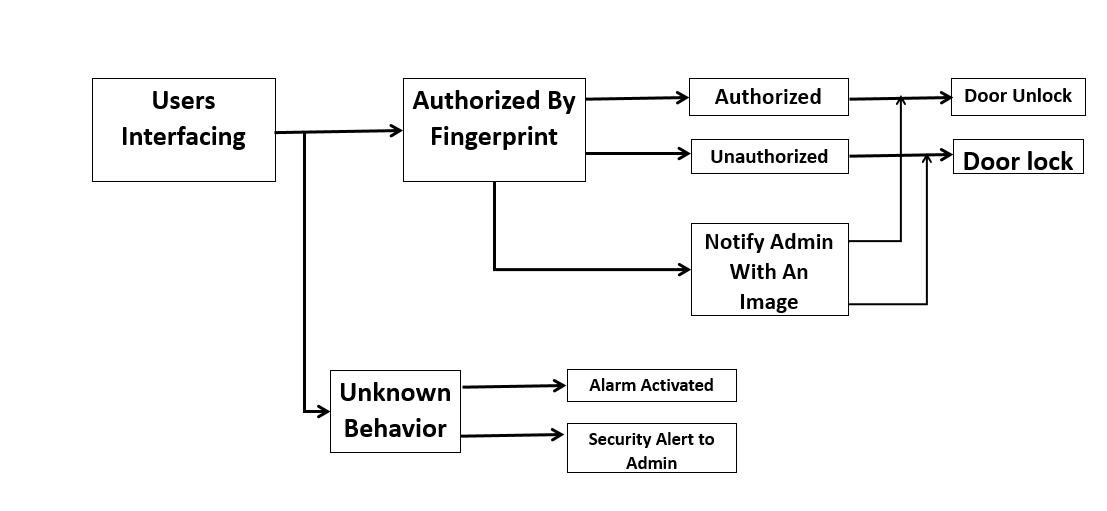
\includegraphics[width=10.0cm]{b1.jpg}
					\caption{Basic Overview}
				\end{center}
			\end{figure}
			When a message was received from the GSM then the micro controller will display that message on LCD at the end
			of the message a number is received based on that number the micro controller will does the coresponinding operation
			to that number like switching the devices ON and OFF. and the date and time of that message received is displayed
			on LCD display.
			\section{Background}
			\section*{Security in the Early Days}
			The home alarm system as we know it today wasn't present during the Stone Age. Cavemen used other means of protection to keep predators at bay. Initially, they used branches and rocks, and later on they created slingshots, and bows and arrows. As time progressed, domesticated wolves were used to protect homes. People would rescue abandoned wolf cubs and raise them to protect their possessions. Eventually, this lead to the guard dogs we know today. In ancient Egypt, around 3150 BC, people would dig trenches around their dwellings, towns, and fortresses. These trenches, also known as moats, were filled with water and used to protect the people from intruders. With the growth of businesses and business ownership during the mid-1700s, people started using security guards to protect their properties. The royals also used security guards for their personal protection. Today, the human touch is still used to offer protection.
			\section*{Home Security Systems Today}
			Today's home security systems are either linked to a landline, or cellular or broadband connection. When the alarm is set off, any one of these three systems can communicate with the monitoring center. If you don't turn off the alarm within a certain period, the center will call you to inquire about the alarm. If it's a false alarm, you must provide your password to stop all further action. If no password is given, or if you don't respond to the call, the police will be sent over to your resident to ensure that there's no burglary taking place. Some home alarm systems can be controlled through your cell phone or tablet. In addition to arming and disarming the alarm system, mobile access to your alarm system can come with other features. You can, for instance, unlock and lock doors, turn the lights on or off, set the thermostat, and more. You can also install a security system with cameras that record every action that occurs on your property. This type of security is often used by business owners. Also, if you're renting a home, or if you plan on moving in a few years, you can install a wireless alarm. This allows you to take your alarm system with you when you move. Some other features that are available when it comes to home security include a glass break sensor, smoke detectors, flood sensors, and carbon monoxide and motion detectors.\\
			
			\section{Aim of this Project}
			The aim of our project is to provide privacy and security to a particular Home or companies from remote loca-
			tions from a central Server system. The idea of having a full control over the places where we live and work has always
			been a fascinating subject to fantasize no matter at what age! As the technology improved in recent decades, human
			being gained more power on controlling various devices indoors. However, having this control remotely still remains
			an incomplete yet developing matter in industry.
			The Project entitled SMART SECURITY SYSTEMS highlights the above mentioned issue and oers ways to
			overcome this need by employing two of the most widely used features of todays technology SMS to be applied as a
			bridge in between human and fully automated buildings, GSM standard which ensures perfect compatibility between
			networks and mobile phones in any location.
			In this project, the system allows the home owner or company owner to monitor and control the house security like
			Whose entered, Door lock or door unlocked, which can be switched on or o via the mobile phone set by sending
			commands in the form of SMS and also the home owner can receive the appliances status.
			\section{History}
			According to the Bureau of Justice Statistics, household burglaries in the United States have declined by 56 percent from 1994 to 2011. It's believed that residential security systems are partly responsible for this decline. Burglars are less likely to break into a home that's secured with an alarm system. If a secured house is invaded, an audible alarm system will often scare off the criminals and stop them in their tracks. Technological developments have made today's home alarm systems ultra-modern, high-tech gadgets. To understand how these developments came about, it's worth exploring the history of home security.\\
			
			\section{ Methodology}
			
			The overall structure of the proposed system is shown in Figure 1.2. The proposed system consists of a digital door lock, two Atmega 8 control board that is mounted in the lock, and the end-user’s mobile device.
			The controller detects physical impacts applied by a visitor, and notifies the user’s mobile device. The controller detects if a invalid fingerprint error occurs more than a certain number of times, and uses the camera to capture an image of the visitor. It then transfers the image to the user’s mobile device. All of the access records are stored in the controller’s database, which can be queried via the user’s mobile device.
			\begin{figure}[ht!]
				\begin{center}
					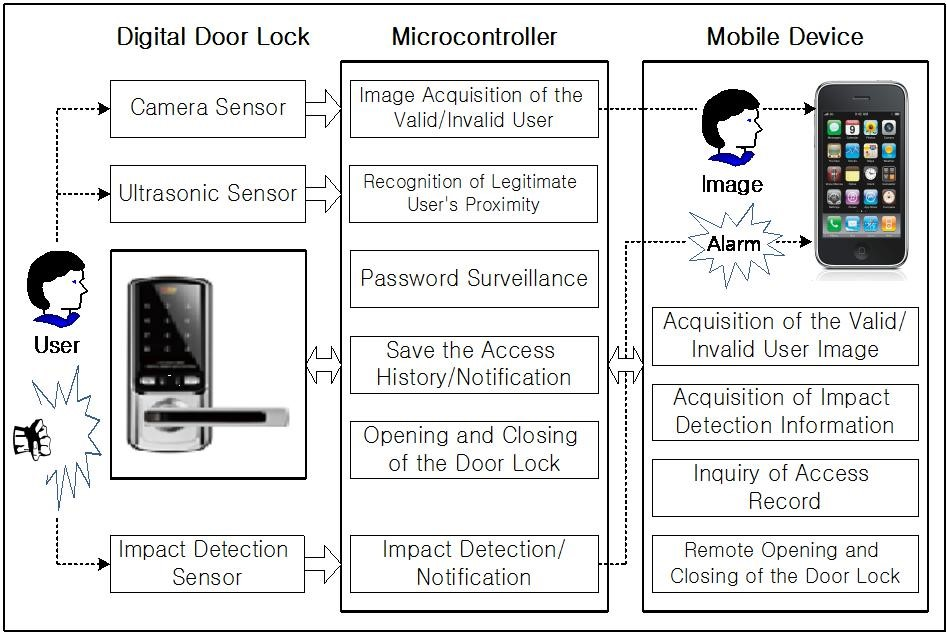
\includegraphics[width=13.0cm]{f1.jpg}
					\caption{Methodology [16]}
				\end{center}
			\end{figure}
			If a visitor has lost his key, his image is captured and transferred to the user’s mobile device by pressing a specific key; the user can then control the door lock remotely after verifying whether the visitor is valid. Another important function of the controller is automatically opening or closing the door when a valid user comes near. When a valid user accesses the gate holding an object, because it is difficult to operate the door lock, the controller communicates with the user’s mobile device via wireless and opens the door lock automatically.
			
			The mobile device acquires the impact detection information and the invalid visitor image information from the controller, and then the user can take appropriate action. Further, if the user acquires image information for a valid visitor, it is possible to open or close the door lock remotely. It is also possible to query the incoming and outgoing
			
			\section{Significance of this Work}
			The main features of the proposed system are as follows. First, it has impact detection
			and alarm functions. This is to detect an intruder who tries to invade by applying physical
			force to the lock. Second, it has an image transfer function. Generally, an attacker who.does not know the password will make a variety of attempts. Therefore, if an attacker
			mistypes the password or fingerprint is not recognized more than a given number of times, the system obtains images of
			the intruder and transfers them to the mobile device.
			Third, the user can query the records of detected face and all incoming and
			outgoing records that are stored in the database. Fourth, the system can open the door lock
			in real-time after recognizing a visitor’s image. If a visitor forgets the password, he can
			type a code into the door lock; then, the door lock system transmits his image to the
			mobile device user. The user can remotely control the door lock after reviewing the
			image. Fifth, the controller can detect a valid user approaching the digital door lock, if he
			is carrying the mobile device, and will open or close the door lock automatically.
			
			\section{Outline}
			The controller detects physical impacts applied by a visitor, and notifies the user’s
			mobile device. The controller detects if a password error occurs more than a certain
			number of times, and uses the camera to capture an image of the visitor. It then transfers
			the image to the user’s mobile device. All of the access records are stored in the
			controller’s database, which can be queried via the user’s mobile device.
			If a visitor has lost his key, his image is captured and transferred to the user’s mobile
			device by pressing a specific key; the user can then control the door lock remotely after
			verifying whether the visitor is valid. Another important function of the controller is
			automatically opening or closing the door when a valid user comes near. When a valid
			user accesses the gate holding an object, because it is difficult to operate the door lock,
			the controller communicates with the user’s mobile device via Bluetooth and opens the
			door lock automatically.
			The mobile device acquires the impact detection information and the invalid visitor
			image information from the controller, and then the user can take appropriate action.
			Further, if the user acquires image information for a valid visitor, it is possible to open or
			close the door lock remotely. It is also possible to query the incoming and outgoing 
			\section{Conclusion}
			The GSM and IOT based advance security system has been designed and tested with the mobile
			network. The user can get alerts anywhere through the GSM technology thus making the
			system location independent. A flexible way to control and explore the services of the mobile,
			AT commands is used in the system. The communication of home is only through the SMS
			which has been tested with the mobile networks and is working on any mobile network.
			The web camera based security system is very easy, user friendly and software has many
			features. It will be more easy to use IP camera instead of web camera. However, the cost of IP
			camera is more. Similar softwares are available on internet which will perform the same task.
			This type of system is useful when the owner is out of station and the home is locked. By
			installing the web camera at the door site, intruder can be detected and owner can receive a \\
			mail telling the intruder entry in a home. If the nearby police station email id is also
			configured in the system, then the intrusion mail can be received by police also and necessary
			action can be taken.
			The system has tested on the model of smart home and further it will be tested in actual
			home. The complexity of the algorithm of the system can be increased by introducing number
			of sensors to make the energy efficient home. 
			\chapter{Literature Review }
			Seo et al. [3] studied convenient digital door lock functions, such as remote control via the integration of mobile devices and key sharing. Lee et al. [4] proposed a method for detecting an accessing object and transmitting the object image. Kwak et al. [5] studied a method for opening and closing the door lock using voice recognition, without using a network. Potts et al. [6] proposed a security system that interfaces with an Android mobile device. The mobile and security system communicate via Bluetooth in a short range. Choi et al. [7] developed an application for communication between devices for transferring the state of the alarms generated in a home through a door lock in the neighborhood.
			
			Hassan et al. [9] and Satti et al. [10] studied face recognition for the door lock open. In particular, the application of Satti et al. transfers the SMS about the legitimacy of the user to the mobile device. However, both of them cannot be a perfect IoT application because the door locks are not controlled by the mobile device remotely. Studies of Park et al. [11] and Verma et al. [12] are related to security applications for home automation. Studies of Khiyal et al. [14] and Ogri et al. [15], are initial studies [13] for remotely controlling a door lock, which cannot be classified also into application of the complete IoT.
			
			The system proposed in this study strengthens the security functions. For example, if a physical impact is added to the intrusion attempt, the system notifies the user of the intrusion through the user’s mobile device. Further, if someone inputs erroneous pass-codes more than a certain number of times, the system captures and transmits an image of the person [8].
			
			To reduce the burden on the network, the proposed system transmits an image only when the input pass-code fails, unlike [4], which transmits a video of all accessing objects. In addition, it provides basic functions, such as remote control access and viewing all incoming and outgoing information that has been recorded on the system.
			
			\section{Existing  technologies related to our project}
			The proposed system provides strengthened security functions that can transfer recorded images to a user’s mobile device when an invalid user attempts an illegal operation; it can also deliver alarm information to the mobile device when the door lock is physically damaged. The proposed system enables a user to check the access information and remotely operate the door lock to enhance convenience.\\
			
			\newpage
			
			\begin{center}
				\begin{table}[h!]
					\centering
					\begin{tabular}{|p{2cm}|p{6cm}|p{5cm}|}
						\hline
						Study (Year) & Main Function & Networking\\
						\hline	
						(2015) & [3]Connecting to mobile devices,Key sharing,mobile device,Access notification & Connection to a mobile device,via Bluetooth\\
						\hline
						(2014) & [4] Image transfer & Connection of mobile devices\\
						\hline
						(2012) & [5] Door opening and closing by speech recognition & –	\\
						\hline
						(2012) & [6] Controlling door lock in a short range with a mobile application & Communication via Bluetooth\\
						\hline
						(2011) & [7] Diffusion of alarm using the door lock & Interconnection of door locks\\
						\hline
						(2012) & [9] Face Recognition & –\\
						\hline
						(2015) & [10] Face Recognition and automatic open & Sending SMS to Mobile phone\\
						\hline
						(2015) & [11] Door Lock for the home automation & –\\
						\hline
						(2010) & [12] Security application for door lock & –\\
						\hline
						(2009) & [14] Basic applications for remote control & Remote control\\
						\hline
						(2013) & [15] Impact detection / notification,Image transfer,Recording access information,Image recognition / remote control,Recognition of user proximity and automatic open & Connection to a	mobile device\\
						\hline	
					\end{tabular}
					\caption{Existing  technologies related to our project}	
				\end{table}
			\end{center}
			The prevention of unauthorized entry into buildings
			through the main doors is done by using ordinary,
			electronically operated locks, digital codes and biometrics
			technique like the finger print technology or some are
			based on thumb printing only. Nowadays, advanced
			automatic door security systems are available with the use
			of palmtop recognition systems face recognition systems,
			face detection systems, wireless sensors, PIR sensors,
			RFID techniques, smart cameras and many more that helps
			people to make their home or organizations secure from
			long distance. Hence, people need not to be worry about
			the home security though they are away from home.
			\section{Introduction  (Study of papers)}
			Recently, digital door locks have been widely used as part of the IoT (Internet of Things). However, the media has reported digital door locks being opened by invalid users to invade homes and offices. In this study, a digital door lock system that can work with the IoT environment is proposed. It is designed and implemented to enhance security and convenience.
			
			The proposed system provides strengthened security functions that can transfer recorded images to a user’s mobile device when an invalid user attempts an illegal operation; it can also deliver alarm information to the mobile device when the door lock is physically damaged. The proposed system enables a user to check the access information and remotely operate the door lock to enhance convenience.
			Security represents protection of our life and assets.
			Ensuring safety of peoples and their valuable things is very
			important for the prevention of illegal handling. Hence,
			mainly focusing on door lock security or gate security is
			very important to avoid the further problems in monitored
			area. Even with the use of mechanical locks, the crime,
			robberies get happened due to the fact that such locks were
			easily broken. So, there is a need to invent other kind of
			locks which cannot be easily broken. So, many authors
			present different kinds of digital door locks, automatic
			password based door locks, software based door locks etc.
			which have been widely used in houses and offices.
			\\
			In latest password based system, a more advanced system
			develops which communicates the owner of the office
			or house, when any unauthorized person tries to open the
			code, by giving correct code as well. While closing the
			door of office/home, the owner has to press the „0‟ key
			available on the hex keypad and leave the system. The
			system developed by Annie P. Oommen et. al.  allows
			for changing the password. To open the lock, the entered
			password must matches with the changed one. In some
			systems the security dial-up enables through the GSM
			modem , when the unauthorized person enters an invalid
			password then the controller informs to the owner through
			GSM modem. Latest security system  is designed where
			the locking security system can be enhanced with the help
			of RF and GSM wireless technology by using a 4 digit
			password which provides the authentication.
			Keywords: Door Lock Security, GSM, RFID, SMS, Sensors, Camera,
			Alarm, Biometrics, WI FI, Password, Internet of things
			\section{Research Approach}
			Redefining 'security' has recently become something of a cottage industry. 1 Most
			such efforts, however, are more concerned with redefining the policy agendas of
			nation-states than with the concept of security itself. Often, this takes the form of
			proposals for giving high priority to such issues as human rights, economics, the
			environment, drug traffic, epidemics, crime, or social injustice, in addition to the
			traditional concern with security from external military threats. Such proposals are
			usually buttressed with a mixture of normative arguments about which values of
			which people or groups of people should be protected, and empirical arguments as
			to the nature and magnitude of threats to those values. Relatively little attention is
			devoted to conceptual issues as such. This article seeks to disentangle the concept of
			security from these normative and empirical concerns, however legitimate they
			may be.
			Cloaking normative and empirical debate in conceptual rhetoric exaggerates the
			conceptual differences between proponents of various security policies and impedes
			scholarly communication. Are proponents of economic or environmental security
			using a concept of security that is fundamentally different from that used by
			Realists? Or are they simply emphasizing different aspects of a shared concept? Do
			those who object to 'privileging' the nation-state rather than, say, the individual or
			humanity share any conceptual views with students of 'national security'? \\
			\\
			it is important to be clear about the limits of this approach. Explicating the
			concept of security does not provide empirical propositions, theories, or analytical
			frameworks. Although clear concepts are useful for constructing propositions.
			theories, and analytical frameworks, they are not a substitute for them. 
			\begin{center}
				\begin{table}[h!]
					\centering
					\begin{tabular}{|p{.8cm}|p{3cm}|p{3cm}|p{3cm}|p{4.5cm}|p{1cm}|}
						\hline
						S.NO. & Artical & Authpr & Publication & CONCLUSION &YEAR \\ \hline
						
						1. & Security and Usability Improvement on a Digital Door Lock System based on Internet of Things & Ilkyu Ha &	Researchgate (December 2016) & In this paper we get an algorithm for implementation of digital door lock & 2015 \\
						\hline
						2. & Technology trends and prospects of development of IoT (M2M) & C. Pyo, H. Gang, N. Kim and H. Bang & OSIA Standards Technology Review, vol. 26, no. 2, & This article was helpful for understanding the concept of internet of things & 2013\\
						\hline
						3. & A low cost GSM/GPRS based wireless home security system & Yanbo Zhao ,  Zhaohui Ye	& IEEE Transactions on Consumer Electronics ( Volume: 54, Issue: 2 ) & In this paper we found that how we can implement a low cost wireless security system & 2008\\
						\hline
						4. & On-line fingerprint verification & A. Jain , Lin Hong , R. Bolle & IEEE Transactions on Pattern Analysis and Machine Intelligence ( Volume: 19, Issue: 4) & This paper was helpful in understanding the concept of fingerprint verification & 1997\\
						\hline
						5. & A door-opening system using a low-cost fingerprint scanner and a PC &	M. Faundez-Zanuy & IEEE Aerospace and Electronic Systems Magazine ( Volume: 19, Issue: 8) & This paper helped us to develop a low cost fingerprint access door lock systems & 2004\\
						\hline
						6. & Remote Monitoring Intelligent System Based on Fingerprint Door Lock & Wu Ping ;  Wu Guichu ;  Xie Wenbin ;  Lu Jianguo ;  Li Peng & IEEE Intelligent Computation Technology and Automation (ICICTA) & In this paper we get algorithms for monitoring of security system based on fingerprint & 2010\\
						\hline
						7. & A camera-based system for tracking people in real time & J. Segen & IEEE & This paper was helpful for development of camera on a system which can monitor real time tracking & 1996\\
						\hline
						8. & Security system with maskable motion detection and camera with an adjustable field of view & Jennifer L. Randall & Grant, US6727938 B1 & In this paper we found algorithm for implement a motion detection system & 1997\\
						\hline
						9. & Design and Implementation of Security Systems for Smart Home based on GSM technology & Jayashri Bangali and Arvind Shaligram & International Journal of Smart Home & This papers helped us to know interfacing of GSM technology with security system & 2013\\
						
						
						
						\hline
						
					\end{tabular}
					\caption{Research Approch}	
				\end{table}
				
			\end{center}
			\newpage
			\section{Modules of project }
			The design of a biometric and web cam based door locking security system using IOT and MATLAB is a complex design which
			comprises of so many modules (parts) brought together to form the overall design. Each of these modules is
			made up of discrete components and modules that are joined together to achieve a particular purpose. 
			These separate modules are: The Power Supply Unit, The Buzzer Unit, The micro controller Unit, Webcam unit, Biometric unit, GSM unit, Image processing unit
			Switching unit.
			These different units can be function alone, for the desired result they all need to function together. We have divided our proposed system into four Module which is as follow.
			\subsection{Survey}
			The researchers gathered information from different sources which give appropriate ideasor what parts to be used in every circuitry involved in this project. Keypad interfacing tomicrocontroller using embedded C was the hardest part ever encountered during thedevelopment stage. From a step by step process, researchers started from writing simplecode to more complex. After everything is fixed and tested in virtual simulation, the researchers soldered everything for implementation stage. Researchers faced many problems on hardware such as fine tuning every sensor to work simultaneously with the burnt program inside the microcontroller. By eliminating those problems gives good andaccurate anticipated result. Same project could have been designed with 8051 microcontroller,Arduino
			\subsection{Study of Software and Hardware}
			\begin{enumerate}
				\item Study of required software (ATmel studio, Proteus Design Suit, Microchip, MATLAB, IOT, )
				\item Study of required hardware and component (Atmega 8, RS305 Fingerprint sensor, GSM Module, Motion Sensor, ESP 8266 wifi Module, LCD)
			\end{enumerate}
			\subsection{Design of the Advance Security System}
			\begin{enumerate}
				
				\item Overall Structure of the Proposed System
				\item Main Features of the Proposed System
			\end{enumerate}
			\subsection{Implementation}
			\begin{enumerate}
				
				\item Hardware Components and Configuration of the Proposed System
				\item Apps for Remote Control
				\item Testing
			\end{enumerate}
			\newpage
			\chapter{System Architecture}
			\section{Overview}
			There are two parts in our project. They are the
			security system and the load controlling system. In the
			security system we use several sensors such as
			Biometric sensor, Webcam, motion sensor. In
			the load controlling system we use relay to on or off the
			load. We have used GSM module to send message to a
			subscriber identification number about security purpose. We have also used this GSM module to control load from remote area. The whole project have been designed in the Proteus software. Each part of our project has been discussed in
			details 
			\subsection{Load controlling system}
			Protection of home main door is the important part in
			security system which done in this system by using
			electromagnetic lock in conjunction with fingerprint module. The
			owner using this biometric for valid user which is display
			on LCD and if the fingerprint matched is correct then the
			electromagnetic lock is opened. Otherwise if does not matched, the door will still locked.\\
			In this project the main and second priority unit is load
			control which has been interfaced with microcontroller.
			Load can be turned on or off by sending message from
			mobile phone. In our project we have controlled two
			loads via microcontroller and GSM module. We can
			also receive update of which load is on or which load is
			off if we want to know it.
			\subsection{Motion detector or Theft Detection unit} 
			The motion sensor gives digital output which has been
			used as microcontrollers input. When motion has been
			detected, motion detector gives logical one to the
			microcontroller. Then microcontroller takes necessary
			decision by reading the detector output. As a motion
			sensor we used PIR sensor which allow you to sense
			motion, almost always used to detect whether a human
			has moved in or out of the sensor's range. They are often
			referred to as PIR, "Passive Infrared", "Piezoelectric", or
			"IR motion" sensors. PIRs are basically made of a
			piezoelectric sensor (which you can see above as the
			round metal can with a rectangular crystal in the centre),
			which can detect levels of infrared radiation. The PIR
			sensor itself has two slots in it; each slot is made of a
			special material that is sensitive to IR. The lens used here
			is not really doing much and so we see that the two slots
			can 'see' out past some distance (basically the sensitivity
			of the sensor).\\
			In theft detection system, simple mechanism has been used.
			When a object has been passed through the door wile sensors are on, buzzers and AC bulbs are connected with 220 volt through the relay and detected as per the microcontroller input port. Then microcontroller takes necessary decision by
			reading the input port. When a object has been passed, logic
			high input to the microcontroller pin.
			\begin{figure}[ht!]
				\begin{center}
					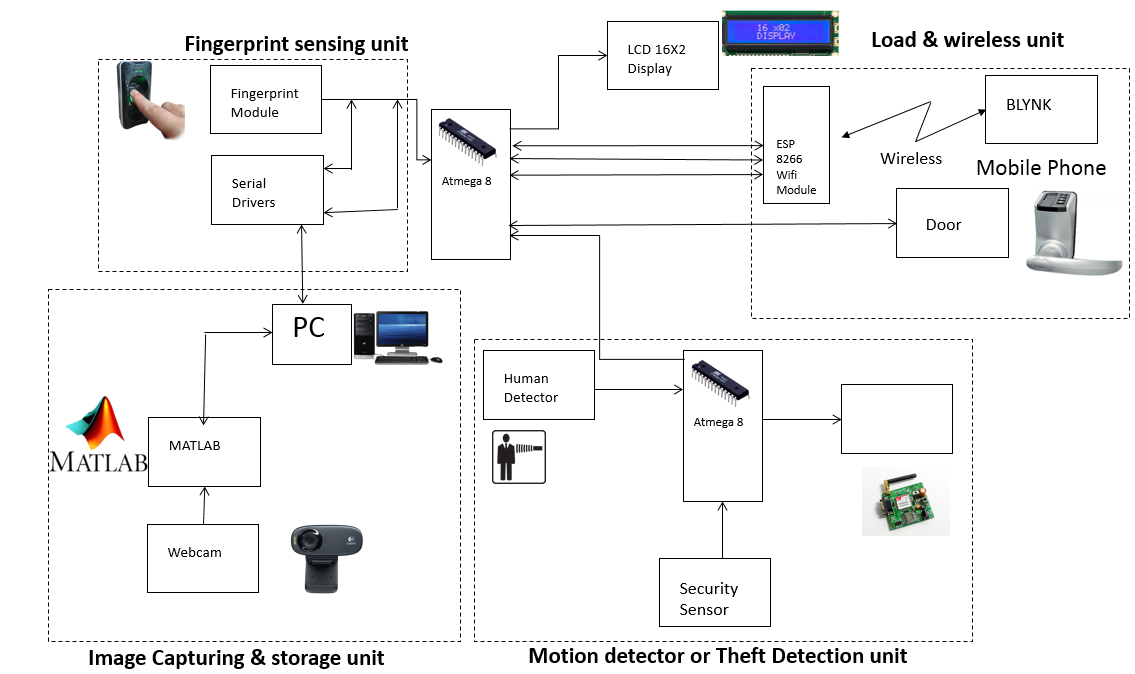
\includegraphics[width=17.0cm]{b2.png}
					\caption{Main Block Diagram}
				\end{center}
			\end{figure}
			\subsection{Fingerprint sensing unit}
			This unit monitors real time fingerprint verification data from 
			doors. This unit has its setting  limitted tryels. Above this  value, the microcontroller sends message to the user‟s mobile phone that the
			someone tryed to acces door and crossed its limitted tryel.
			In case if user is verified than an output will send through the microcontroller to the load for unlock the door. We have used RS305 as fingerprint sensor.
			
			\subsection{Image Capturing \& storage unit}
			By default the first camera is selected, but we can select any of the available devices from the
			listbox .After the device is selected, the camera is interfaced through coding part. Then there is a button
			‘Activate Motion Detection’, through which we can select the mode of our working and the application is set on Whenever any unvalid user tryed to access then application
			starts capturing the images and they are stored into a folder using. At the same time , a wireless signal is transmitted to the receiver through ESP8266 module using blink application and wait for desired action taken from the owner side.
			\section{Reaction of sensors \& Flow chart}
			\subsection{Reaction of Sensors}
			Figure 3.2 shows the reaction time of each sensor. All of the sensors act to actions of the valid and invalid user in 2 seconds. For example, the ultrasonic sensor can take from 1.6 seconds to 1.8 seconds to check a valid user and open the door. One of the most important features of our proposed system is to check an invalid password of an invalid user. It takes 1.41 seconds on average to detect an invalid password, take a picture of the user and send the picture to a mobile device.
			\begin{figure}[ht!]
				\begin{center}
					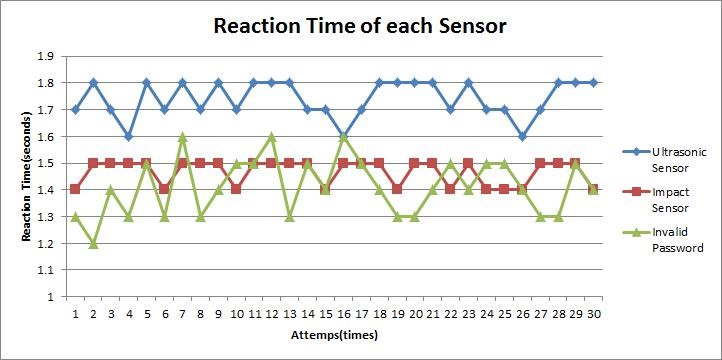
\includegraphics[width=12.0cm]{f5.jpg}
					\caption{Reaction of each sensors [16]}
				\end{center}
			\end{figure}
			The proposed digital door lock system in this study has several implementation problems. The first problem concerns the image captured by the camera's sensor when an incorrect password is entered. If the invader intentionally covers the camera lens or deviates the focus from him, it will be impossible to collect an accurate image. Second, since the shock sensor senses a certain amount of impact whenever the door opens or closes, it is difficult to distinguish an abnormal impact. These problems will be resolved as future challenges.
			\subsection{Flow Chart}
			In this flow chart two cases are discussed in which one is for valid user and another one is for invalid user all the activity of these usr will be capture and can be store and also there are limited no of tryels for each.Besides, various sensors for proximity and intrusion detection are connected to the system. A camera sensor for photographing an image of invalid users is installed, an impact sensor is attached for detecting a physical shock by an invalid user, and an ultrasonic sensor is attached to recognize the proximity of valid users.\\\\
			When an access request is generated by a valid visitor who does not possess the key, the ‘Request’ menu allows the user to check the image of the requester and open the door. The ‘Remote opening’ menu allows for remote door operation. The ‘Option’ menu allows for password management and ‘Bluetooth synchronization (Master mode)’ menu is a setting menu for automatic opening when approaching the door lock. Figure 6 shows the application cases for remote controls. The left side of the top of the figure is the main menu of the App, the right of the top shows the Bluetooth setup button for proximity open and a keypad for the remote open. The left of the bottom of the figure shows a list of the image information that has been captured by physical shock and the input mistake of password. And the right of the bottom shows an image of the item in the list.
			
			
			
			
			\begin{figure}[ht!]
				\begin{center}
					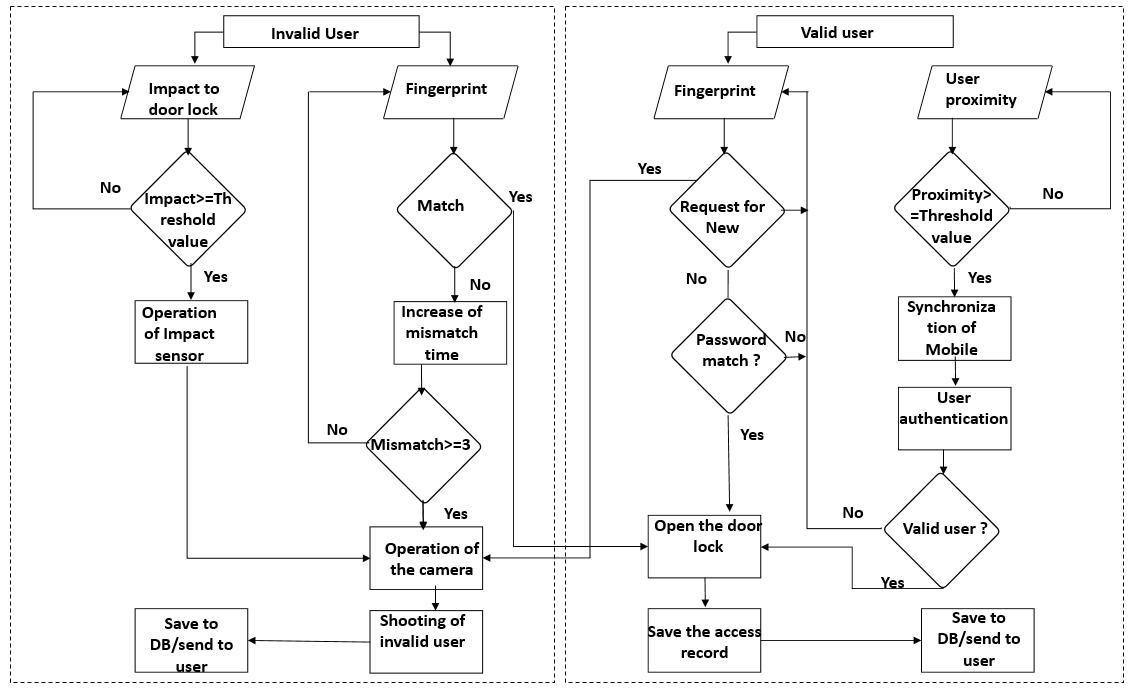
\includegraphics[width=16cm]{f6.png}
					\caption{Flow Chart of Project}
				\end{center}
			\end{figure}
			\section{Algorithm}
			STEP 1  : \hspace{0.2cm} {\bf START}\\
			STEP 2  : \hspace{0.2cm} {\bf FOR} each user\\
			STEP 3  : \hspace{0.6cm} {\bf INPUT} Action\\
			STEP 4  : \hspace{0.6cm} {\bf SWITCH} Action\\
			STEP 5  : \hspace{1cm} {\bf CASE} ``fingerprint"\\
			STEP 6  : \hspace{1.4cm} {\bf IF} fingerprint does not match {\bf THEN} take and send image\\
			STEP 7  : \hspace{1.4cm} {\bf ELSE IF} fingerprint is valid {\bf THEN} open the door\\
			STEP 8  : \hspace{1.4cm} {\bf ELSE IF} number of mismatch greater then 3 {\bf THEN} take and send image\\
			STEP 9  : \hspace{1.8cm} {\bf ELSE} go to STEP 2\\
			STEP 10 : \hspace{1cm} {\bf CASE} ``impact"\\
			STEP 11 : \hspace{1.cm} Impact Sensor operation\\
			STEP 12 : \hspace{1.4cm} {\bf IF} impact value greater then threshold valu {\bf THEN} camera sensor operation\\
			STEP 13 : \hspace{1.4cm} {\bf ELSE} go to STEP 2\\
			STEP 14 : \hspace{1cm} {\bf CASE} ``proximity"\\
			STEP 15 : \hspace{1.4cm} {\bf IF} distance greater then threshold value {\bf THEN} mobile device synchronization\\
			STEP 16 : \hspace{1.6cm} {\bf IF} valid user {\bf THEN} open the door\\
			STEP 17 : \hspace{1.6cm} {\bf ELSE} go to STEP 2\\
			STEP 18 : \hspace{1.4cm} {\bf ELSE} go to STEP 2\\
			STEP 19 : \hspace{0.2cm} {\bf END}
			
			\chapter{\bf Implementation of Project }
			\section{Software Requirement }
			\subsection{ATmel Studio}
			AVR Studio 6 is a software development environment developed by Atmel. It is meant to replace AVR Studio 5 going forward providing a single development platform for Atmel's 8-bits, 32-bits and ARM Cortex-M families of AVR microcontrollers.AVR is a family of microcontrollers developed by Atmel beginning in 1996. These are modified Harvard architecture 8-bit RISC single-chip microcontrollers. AVR was one of the first microcontroller families to use on-chip flash memory for program storage, as opposed to one-time programmable ROM, EPROM, or EEPROM used by other microcontrollers at the time.
			
			AVR microcontrollers find many applications as embedded systems; they are also used in the Arduino line of open source board designs.
			
			\begin{figure}
				\begin{center}
					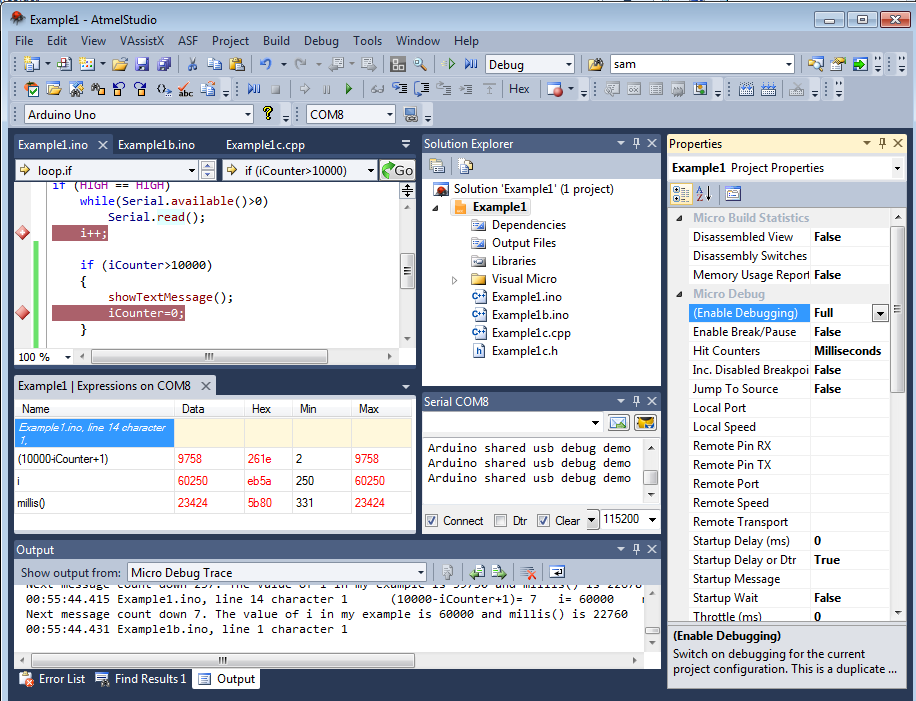
\includegraphics[width=10.0cm]{cc.png}
					\caption{ATmel Studio Interface}
				\end{center}
			\end{figure}
			\subsection*{Brief History}
			
			The AVR architecture was conceived by two students at the Norwegian Institute of Technology (NTH),[1] Alf-Egil Bogen[2] and Vegard Wollan.[3]
			
			The original AVR MCU was developed at a local ASIC house in Trondheim, Norway, called Nordic VLSI at the time, now Nordic Semiconductor, where Bogen and Wollan were working as students.[citation needed] It was known as a μRISC (Micro RISC) and was available as silicon IP/building block from Nordic VLSI. When the technology was sold to Atmel from Nordic VLSI, the internal architecture was further developed by Bogen and Wollan at Atmel Norway, a subsidiary of Atmel. The designers worked closely with compiler writers at IAR Systems to ensure that the AVR instruction set provided efficient compilation of high-level languages.
			Atmel says that the name AVR is not an acronym and does not stand for anything in particular. The creators of the AVR give no definitive answer as to what the term "AVR" stands for.However, it is commonly accepted that AVR stands for Alf and Vegard's RISC processor.Note that the use of "AVR" in this article generally refers to the 8-bit RISC line of Atmel AVR Microcontrollers.
			
			Among the first of the AVR line was the AT90S8515, which in a 40-pin DIP package has the same pinout as an 8051 microcontroller, including the external multiplexed address and data bus. The polarity of the RESET line was opposite (8051's having an active-high RESET, while the AVR has an active-low RESET), but other than that the pinout was identical.
			
			The AVR 8-bit microcontroller architecture was introduced in 1997. By 2003, Atmel had shipped 500 million AVR flash microcontrollers. The Arduino platform for simple electronics projects was released in 2005 and featured ATmega8 AVR microcontrollers.
			\subsection{Proteus Design Suite}
			The Proteus Design Suite is a proprietary software tool suite used primarily for electronic design automation. The software is used mainly by electronic design engineers and technicians to create schematics and electronic prints for manufacturing printed circuit boards.
			Proteus is a simulation and design software tool developed by Labcenter Electronics for Electrical
			and Electronic circuit design. It also possess 2D CAD drawing feature. It deserves to bear the tagline ``From concept to completion”.
			It was developed in Yorkshire, England by Labcenter Electronics Ltd and is available in English, French, Spanish and Chinese languages.
			\subsection*{History}
			The first version of what is now the Proteus Design Suite was called PC-B and was written by the company chairman, John Jameson, for DOS in 1988. Schematic Capture support followed in 1990, with a port to the Windows environment shortly thereafter. Mixed mode SPICE Simulation was first integrated into Proteus in 1996 and microcontroller simulation then arrived in Proteus in 1998. Shape based autorouting was added in 2002 and 2006 saw another major product update with 3D Board Visualisation. More recently, a dedicated IDE for simulation was added in 2011 and MCAD import/export was included in 2015. Feature led product releases are typically biannual, while maintenance based service packs are released as required.
			\subsection*{Features}
			ISIS has wide range of components in its library. It has sources, signal generators, measurement  and analysis tools like oscilloscope, voltmeter, ammeter etc., probes for real time monitoring of the parameters of the circuit, switches, displays, loads like motors and lamps, discrete components like resistors, capacitors, inductors, transformers, digital and analog Integrated circuits, semi-conductor switches, relays, microcontrollers, processors, sensors etc.
			
			ARES offers PCB designing up to 14 inner layers, with surface mount and through hole packages. It is embedded with the foot prints of different category of components like ICs, transistors, headers, connectors and other discrete components. It offers Auto routing and manual routing options to the PCB Designer. The schematic drawn in the ISIS can be directly transferred ARES.
			\begin{itemize}
				\item It is a software suite containing schematic, simulation as well as PCB designing.
				\item ISIS is the software used to draw schematics and simulate the circuits in real time.The simulation allows human access during run time,thus providing real time simulation.
				\item ARES  is used for PCB designing.It has the feature of viewing output in 3D view of the designed PCB along  with components.
				\item The designer can also develop 2D drawings for the product.
			\end{itemize}
			
			
			\begin{figure}[ht!]
				\begin{center}
					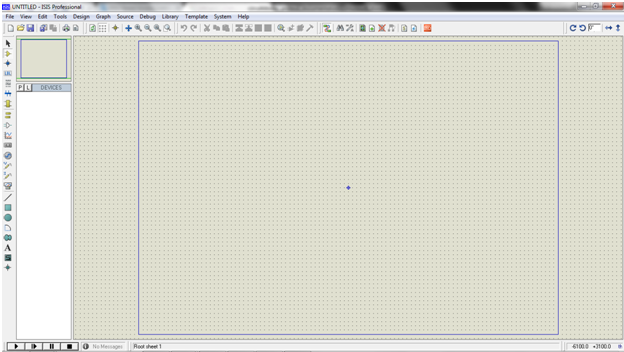
\includegraphics[width=15.0cm]{2.png}
					\caption{Proteus Design Suite Interface}
				\end{center}
			\end{figure}
			\subsection{Microchip}
			
			Studies indicate that up to 60\% of a project’s development cycle can be spent on software development. Microchip’s award-winning software solutions, spanning all of its MCU products, are designed to enable developers to rapidly progress their projects to completion. Below you will find ready-to-use software development solutions and support for Microchip’s 8-, 16- and 32-bit microcontrollers.\\
			A microchip (sometimes just called a "chip") is a unit of packaged computer circuitry (usually called an integrated circuit) that is manufactured from a material such as silicon at a very small scale. Microchips are made for program logic (logic or microprocessor chips) and for computer memory (memory or RAM chips). Microchips are also made that include both logic and memory and for special purposes such as analog-to-digital conversion, bit slicing, and gateways.
			\begin{figure}[ht!]
				\begin{center}
					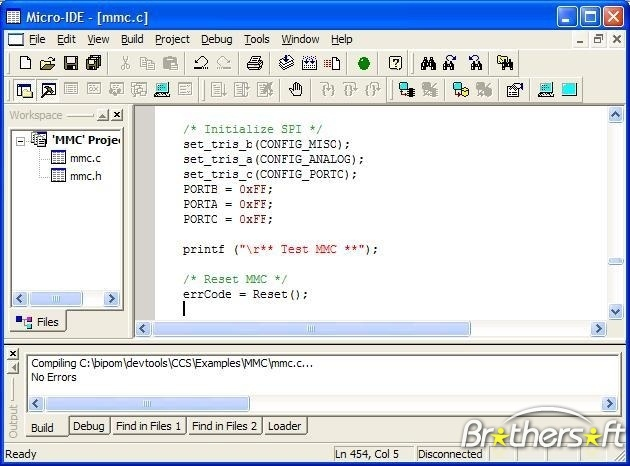
\includegraphics[width=15.0cm]{3.jpeg}
					\caption{Microchip Interface}
				\end{center}
			\end{figure}
			
			
			\subsection*{Microchp Library for Application(MLA)}
			Microchip Libraries for Applications (MLA) includes a combination of source code, drivers, demos, documentation and utilities to help configure software libraries such as USB, graphics, crypto, smart card, and wireless stacks. The MLA software covers all 16-bit PIC24 and dsPIC33 product families, as well as some support for 8-bit PIC16 and PIC18 families.\\
			\subsection*{Embedded Source code}
			Embedded code source includes software from a large network of third party developers as well as software developed by Microchip. Browse and download free code snippets tools and utilities. Premium code with advanced features can also be purchased. Embedded code source includes PIC MCU code or a wide variety of applications including wireless touch sensing and display drivers.\\
			\subsection{MATLAB}
			MATLAB is an interactive system whose basic data element is an array that does not require dimensioning. This allows you to solve many technical computing problems, especially those with matrix and vector formulations, in a fraction of the time it would take to write a program in a scalar noninteractive language such as C or Fortran.The name MATLAB stands for matrix laboratory. MATLAB was originally written to provide easy access to matrix software developed by the LINPACK and EISPACK projects, which together represent the state-of-the-art in software for matrix computation.
			MATLAB has evolved over a period of years with input from many users. In university environments, it is the standard instructional tool for introductory and advanced courses in mathematics, engineering, and science. In industry, MATLAB is the tool of choice for high-productivity research, development, and analysis.
			MATLAB features a family of application-specific solutions called toolboxes. Very important to most users of MATLAB, toolboxes allow you to learn and apply specialized technology. Toolboxes are comprehensive collections of MATLAB functions (M-files) that extend the MATLAB environment to solve particular classes of problems. Areas in which toolboxes are available include signal processing, control systems, neural networks, fuzzy logic, wavelets, simulation, and many others.
			MATLAB is widely used in all areas of applied mathematics, in education and research at universities, and in the industry. MATLAB stands for MATrix LABoratory and the software is built up around vectors and matrices. This makes the software particularly useful for linear algebra but MATLAB is also a great tool for solving algebraic and differential equations and for numerical integration. MATLAB has powerful graphic tools and can produce nice pictures in both 2D and 3D. It is also a programming language, and is one of the easiest programming languages for writing mathematical programs. MATLAB also has some tool boxes useful for signal processing, image processing, optimization, etc.
			\begin{figure}[ht!]
				\begin{center}
					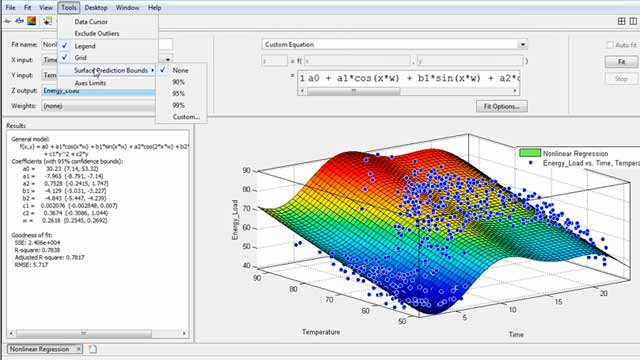
\includegraphics[width=13.0cm]{4.jpg}
					\caption{MATLAB Interface}
				\end{center}
			\end{figure}
			\section*{The MATLAB environment} 
			The MATLAB environment (on most computer systems) consists of menus, buttons and a writing area similar to an ordinary word processor. There are plenty of help functions that you are encouraged to use. The writing area that you will see when you start MATLAB, is called the command window. In this window you give the commands to MATLAB. For example, when you want to run a program you have written for MATLAB you start the program in the command window by typing its name at the prompt. The command window is also useful if you just want to use MATLAB as a scientific calculator or as a graphing tool. If you write longer programs, you will find it more convenient to write the program code in a separate window, and then run it in the command window (discussed in Intro to programming).\\
			
			In the command window you will see a prompt that looks like >> . You type your commands immediately after this prompt. Once you have typed the command you wish MATLAB to perform, press <enter>. If you want to interupt a command that MATLAB is running, type <ctrl> + <c>.\\
			
			The commands you type in the command window are stored by MATLAB and can be viewed in the Command History window. To repeat a command you have already used, you can simply double-click on the command in the history window, or use the <up arrow> at the command prompt to iterate through the commands you have used until you reach the command you desire to repeat.\\
			\section*{The MATLAB Application Program Interface (API)} 
			This is a library that allows you to write C and Fortran programs that interact with MATLAB. It include facilities for calling routines from MATLAB (dynamic linking), calling MATLAB as a computational engine, and for reading and writing MAT-files.
			\section*{The MATLAB mathematical function library} 
			This is a vast collection of computational algorithms ranging from elementary functions like sum, sine, cosine, and complex arithmetic, to more sophisticated functions like matrix inverse, matrix eigenvalues, Bessel functions, and fast Fourier transforms.
			\subsection*{MATLAB Features} 
			\begin{itemize}
				\item It is a high-level language for numerical computation, visualization and application development.
				\item It also provides an interactive environment for iterative exploration, design and problem solving.
				\item It provides vast library of mathematical functions for linear algebra, statistics, Fourier analysis, filtering, optimization, numerical integration and solving ordinary differential equations.
				\item It provides built-in graphics for visualizing data and tools for creating custom plots.
				\item MATLAB's programming interface gives development tools for improving code quality maintainability and maximizing performance.
				\item It provides tools for building applications with custom graphical interfaces.
				\item It provides functions for integrating MATLAB based algorithms with external applications and languages such as C, Java, .NET and Microsoft Excel.
			\end{itemize}
			\subsection{Internet of Things}
			The Internet of things (IoT) is the network of physical devices, vehicles, home appliances, and other items embedded with electronics, software, sensors, actuators, and network connectivity which enable these objects to connect and exchange data. Each thing is uniquely identifiable through its embedded computing system but is able to inter-operate within the existing Internet infrastructure. Experts estimate that the IoT will consist of about 30 billion objects by 2020.\\\\
			The IoT allows objects to be sensed or controlled remotely across existing network infrastructure, creating opportunities for more direct integration of the physical world into computer-based systems, and resulting in improved efficiency, accuracy and economic benefit in addition to reduced human intervention. When IoT is augmented with sensors and actuators, the technology becomes an instance of the more general class of cyber-physical systems, which also encompasses technologies such as smart grids, virtual power plants, smart homes, intelligent transportation and smart cities.
			\begin{figure}[ht!]
				\begin{center}
					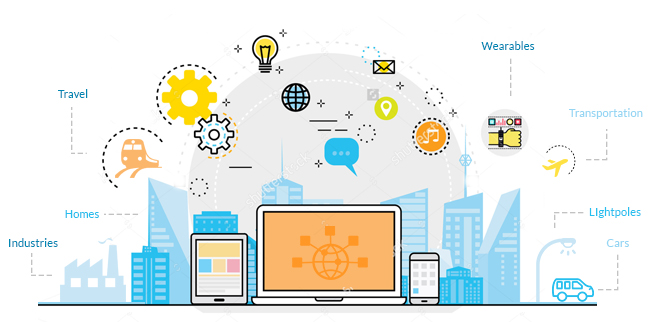
\includegraphics[width=10.0cm]{5.jpg}
					\caption{Internet of Things}
				\end{center}
			\end{figure}
			"Things", in the IoT sense, can refer to a wide variety of devices such as heart monitoring implants, biochip transponders on farm animals, cameras streaming live feeds of wild animals in coastal waters, automobiles with built-in sensors, DNA analysis devices for environmental/food/pathogen monitoring, or field operation devices that assist firefighters in search and rescue operations. Legal scholars suggest regarding "things" as an "inextricable mixture of hardware, software, data and service".
			These devices collect useful data with the help of various existing technologies and then autonomously flow the data between other devices.The term "the Internet of things" was coined by Kevin Ashton of Procter \& Gamble, later MIT's Auto-ID Center, in 1999.
			\section*{Features of IOT}
			\section*{A General Features List for Wireless Nodes}
			The information from looking at multiple examples such as the ones above were translated into the diagram below, in an attempt to capture the typical features that may be encountered.
			An IoT solution will use some of these. Some features may be missing, and all need to be fleshed out. The diagram may be representable in better ways. These points will be addressed in future posts.
			Hopefully the diagram can evolve. Any comments or contributions would be appreciated.
			\subsection{Embedded System}
			An embedded system is a computer that has been built to solve only a few very specific problems and is not easily changed.[1] In contrast, a general-purpose computer can do many different jobs, and can be changed at any time with new programs for new jobs.Embedded systems are not always standalone devices. Sometimes they are built as a set, like the various parts of a car - the radio, the throttle control, the pollution control, etc.[2] Sometimes they can communicate to the internet or a cell-phone network and they may have a USB reader or other connections.
			An embedded system usually does not look like a computer, often there is no keyboard or monitor or mouse. But like any computer it has a processor and software, input and output. The word embedded means it is built into the system. It is a permanent part in a bigger system.\\
			
			\begin{figure}[ht!]
				\begin{center}
					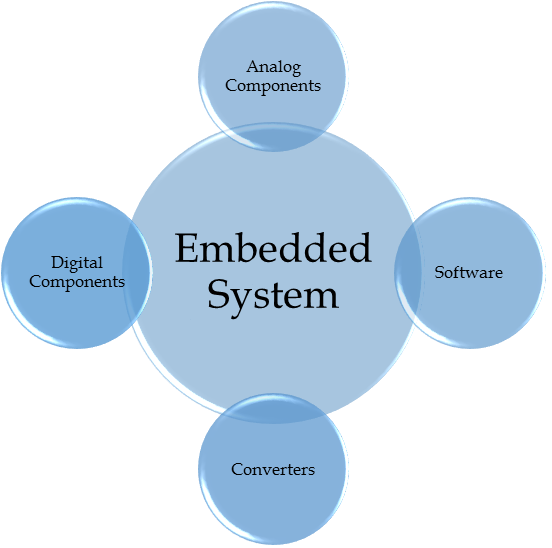
\includegraphics[width=8.0cm]{6.png}
					\caption{Embedded System}
				\end{center}
			\end{figure}
			For example, the controller embedded in an elevator tells the motor to move the elevator to different floors, based on buttons that are pushed. A decoder is embedded in a satellite television set-top box to read a signal from the dish and send something that a TV understands. Often this type of system must do its work in a specific amount of time. This is called real-time computing. If a set-top box got interrupted to do another task, you would see a bad picture on the TV, for example. A general purpose computer will often have short pauses while it does something else, it is not real-time.
			
			Embedded systems control many of the common devices in use today, from card readers in hotel door locks to many controls in a car. They can be small like an MP3 player or a digital camera, to large systems like traffic lights, airplane controls, or assembly line controllers in a factory.
			\subsection*{Common Features}
			\begin{itemize}
				\item Embedded systems are designed to do a specific task, unlike general-purpose computers.
				\item It does not look like a computer - there may not be a full monitor or a keyboard.
				\item Many embedded systems must be able to do things in real-time - in a short amount of time (almost instantly from a human view).
				\item Many embedded systems must be very safe and reliable, especially for medical devices or avionics controlling airplanes.
				\item Starts very quickly. People don't want to wait a minute or two for their car to start or emergency equipment to start.
				\item It may use a special operating system (or sometimes a very small home-made OS) that helps meet these requirements called a real-time operating system, or RTOS.
				\item The program instructions written for embedded systems are referred to as firmware, and are stored in read-only memory or flash memory chips. They run with limited computer hardware resources: little memory, small or non-existent keyboard and/or screen.\\	
			\end{itemize}
			\subsection{Blynk Application}
			Blynk is a Platform with iOS and Android apps to control Arduino, Raspberry Pi and the likes over the Internet. It’s a digital dashboard where you can build a graphic interface for your project by simply dragging and dropping widgets. It’s really simple to set everything up and you’ll start tinkering in less than 5 mins. Blynk is not tied to some specific board or shield. Instead, it’s supporting hardware of your choice. Whether your Arduino or Raspberry Pi is linked to the Internet over Wi-Fi, Ethernet or this new ESP8266 chip, Blynk will get you online and ready for the Internet Of Your Things.
			
			\begin{figure}[ht!]
				\begin{center}
					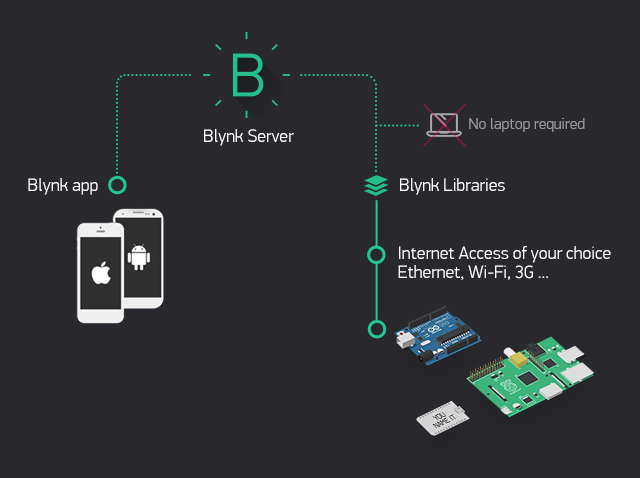
\includegraphics[width=10.0cm]{blynk2.png}
					\caption{Blynk Application}
				\end{center}
			\end{figure}
			\chapter{Hardware Requirement}
			\section{List of Hardware Components}
			\begin{center}
				\begin{table}[h!]
					\centering
					\begin{tabular}{|p{1cm}|p{8cm}|p{1cm}|p{6.5cm}|}
						\hline
						{\bf S.No.} & {\bf Name of Component} & {Quantity} & {\bf Working}\\
						\hline	
						1. & ATmega 8 & 2 & Microcontroller\\
						\hline
						2. & Proximity Sensor  & 1 & For Motion Detection\\
						\hline
						3. & ESP8266 & 1 & For Internet of things communication using blynk\\
						\hline
						4. & L239D & 1 & Motor Driver\\
						\hline
						5. & GSM Module & 1 & For deliver a message on admin phone\\
						\hline
						6. & SIM Card & 1 & For send a alert message to the admin\\
						\hline
						7. & USB to TTL & 1 & For seria communication\\
						\hline
						8. & LCD 16 X 2 & 1 & For display Purpose \\
						\hline
						9. & Relay & 2 & For switching purpose \\
						\hline
						10. & Burzer & 1 & For Alert \\
						\hline
						11. & 7805 Voltage regulator & 3 & For voltage conversion \\
						\hline
						12. & R302 Fingerptint Module & 1 & Fingerprint scanner \\
						\hline
						13. & DVD Drive & 1 & For Door lock unlock process\\
						\hline
						14. & 12v Adaptor & 1 & Power supply \\
						\hline
						15. & Basic Component & NA & LED,Capacitor,Registor,Transistor,Crystal oscillator \\
						\hline
					\end{tabular}
					\caption{List of Hardware Components}	
				\end{table}
			\end{center}
			\section{ATmega 8 Microcontroller }
			The abbreviation of AVR Microcontroller is “Advanced Virtual RISC” and MCU is the short term of the Microcontroller. A Microcontroller is a tiny computer on a single chip and it is also termed as a control device. Similar to a computer, the Microcontroller is made with a variety of peripherals like input \& output units, memory, Timers, serial data communications, programmable. The applications of Microcontroller involve in embedded applications \& automatically controlled devices like medical devices, remote control devices, control systems, office machines, power tools, electronic devices, etc. There are various kinds of Microcontrollers available in the market like 8051, PIC and AVR microcontroller. This article gives a brief information about AVR Atmega8 microcontroller.
			\begin{figure}[ht!]
				\begin{center}
					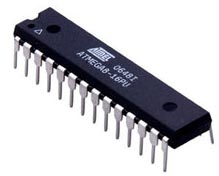
\includegraphics[width=5.0cm]{8.jpg}
					\caption{ATmega 8 IC}
				\end{center}
			\end{figure}
			\subsection{Atmega8 Microcontroller Pin Description}
			The main feature of Atmega8 Microcontroller is that, all the pins of the Microcontroller support two signals except 5-pins. The Atmega8 microcontroller consists of 28 pins where pins 9,10,14,15,16,17,18,19 are used for port B, Pins 23,24,25,26,27,28 and 1 are used for port C and pins 2,3,4,5,6,11,12 are used for port D.\\
			\begin{figure}[ht!]
				\begin{center}
					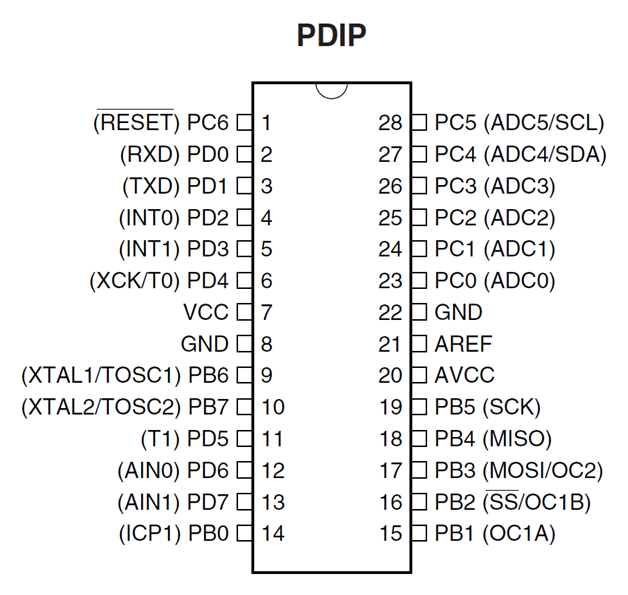
\includegraphics[width=10.0cm]{9.png}
					\caption{ATmega 8 PIN Diagram}
				\end{center}
			\end{figure}
			\begin{itemize}
				\item Pin -1 is the RST (Reset) pin and applying a low level signal for a time longer than the minimum pulse length will produce a RESET.
				\item Pin-2 and pin-3 are used in USART for serial communication
				\item Pin-4 and pin-5 are used as an external interrupt. One of them will activate when an interrupt flag bit of the status register is set and the other will activate as long as the intrude condition succeeds.
				\item Pin-9 \& pin-10 are used as a timer counters oscillators as well as an external oscillator where the crystal is associated directly with the two pins. Pin-10 is used for low-frequency crystal oscillator or crystal oscillator. If the internal adjusted RC oscillator is used as the CLK source \& the asynchronous timer is allowed, these pins can be utilized as a timer oscillator pin.
				\item Pin-19 is used as a Master CLK o/p, slave CLK i/p for the SPI-channel.
				\item Pin-18 is used as Master CLK i/p, slave CLK o/p.
				\item Pin-17 is used as Master data o/p, slave data i/p for the SPI-channel. It is used as an i/p when empowered by a slave \& is bidirectional when allowed by the master. This pin can also be utilized as an o/p compare with match o/p, which helps as an external o/p for the timer/counter.
				\item Pin-16 is used as a slave choice i/p. It can also be used as a timer or counter1 comparatively by arranging the PB2-pin as an o/p.
				\item Pin-15 can be used as an external o/p of the timer or counter compare match A.
				\item Pin-23 to Pins28 have used for ADC (digital value of analog input) channels. Pin-27 can also be used as a serial interface CLK \& pin-28 can be used as a serial interface data
				\item Pin-12 and pin-13 are used as an Analog Comparator i/ps
				\item Pin-6 and pin-11 are used as timer/counter sources.\\
			\end{itemize}
			
			\begin{figure}[ht!]
				\begin{center}
					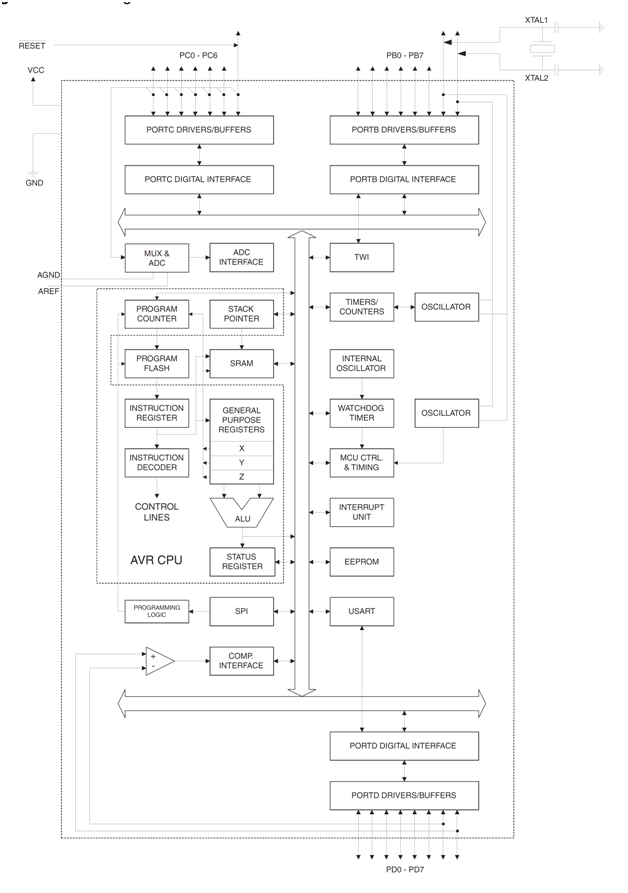
\includegraphics[width=15.0cm]{10.png}
					\caption{ATmega 8 Architecture}
				\end{center}
			\end{figure}
			\section{RS305 Fingerprint Module }
			This is a fingure print sensor module with TTL UART interface for direct connections to microcontroller UART or to PC through MAX232 / USB-Serial adapter. The user can store the finger print data in the module and can configure it in 1:1 or 1: N mode for identifying the person.The FP module can directly interface with 3v3 or 5v Microcontroller. A level converter (like MAX232) is required for interfacing with PC serial port.
			
			Optical biometric fingerprint reader with great features and can be embedded into a variety of end products, such as: access control, attendance, safety deposit box, car door locks
			\begin{figure}[ht!]
				\begin{center}
					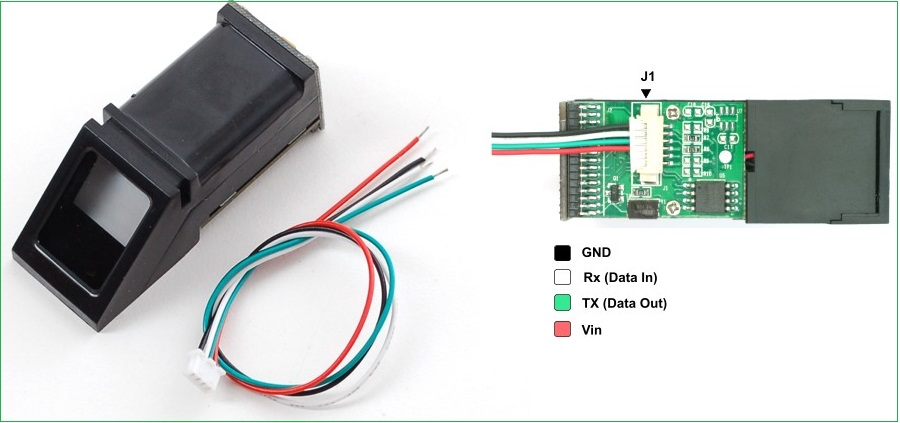
\includegraphics[width=10.0cm]{11.jpg}
					\caption{RS305 Fingerprint Module}
				\end{center}
			\end{figure}
			
			\subsection*{Features}
			\begin{itemize}
				\item Integrated image collecting and algorithm chip together, ALL-in-One
				\item Fingerprint reader can conduct secondary development, can be embedded into a variety of end products
				\item Low power consumption, low cost, small size, excellent performance
				\item Professional optical technology, precise module manufacturing techniques
				\item Good image processing capabilities, can successfully capture image up to resolution 500 dpi
			\end{itemize}
			\subsection*{Specification}
			\begin{itemize}
				\item Fingerprint sensor type: Optical
				\item Sensor Life: 100 million times
				\item Static indicators: 15KVBacklight: bright green
				\item Interface: USB1.1/UART(TTL logical level)
				\item RS232 communication baud rate: 4800BPS~115200BPS changeable
				\item Dimension: 55*32*21.5mm
				\item Image Capture Surface 15—18(mm)
				\item Verification Speed: 0.3 sec
				\item Scanning Speed: 0.5 sec
				\item Character file size: 256 bytes
				\item Template size: 512 bytes
				\item Storage capacity: 250
				\item Security level: 5 (1,2,3,4,5(highest))
				\item False Acceptance Rate (FAR) :0.0001%
				\item False Rejection Rate (FRR): 0.1%
				\item Resolution 500 DPI
				\item Voltage :3.6-6.0 VDC
				\item Working current: Typical 90 mA, Peak 150mA
				\item Matching Method: 1: N
				\item Operating Environment Temperature: -20 to 45° centigrades
				
			\end{itemize}
			\section{GSM Module }
			GSM/GPRS module is used to establish communication between a computer and a GSM-GPRS system. Global System for Mobile communication (GSM) is an architecture used for mobile communication in most of the countries. Global Packet Radio Service (GPRS) is an extension of GSM that enables higher data transmission rate. GSM/GPRS module consists of a GSM/GPRS modem assembled together with power supply circuit and communication interfaces (like RS-232, USB, etc) for computer. GSM/GPRS MODEM is a class of wireless MODEM devices that are designed for communication of a computer with the GSM and GPRS network. It requires aSIM (Subscriber Identity Module) card just like mobile phones to activate communication with the network. Also they have IMEI (International Mobile Equipment Identity) number similar to mobile phones for their identification. A GSM/GPRS MODEM can perform the following operations: 
			\begin{enumerate}
				\item Receive, send or delete SMS messages in a SIM.
				\item Read, add, search phonebook entries of the SIM.
				\item Make, Receive, or reject a voice call.
			\end{enumerate}
			
			
			The MODEM needs AT commands, for interacting with processor or controller, which are communicated through serial communication. These commands are sent by the controller/processor. The MODEM sends back a result after it receives a command. Different AT commands supported by the MODEM can be sent by the processor/controller/computer to interact with the GSM and GPRS cellular network. capabilities.
			\begin{figure}[ht!]
				\begin{center}
					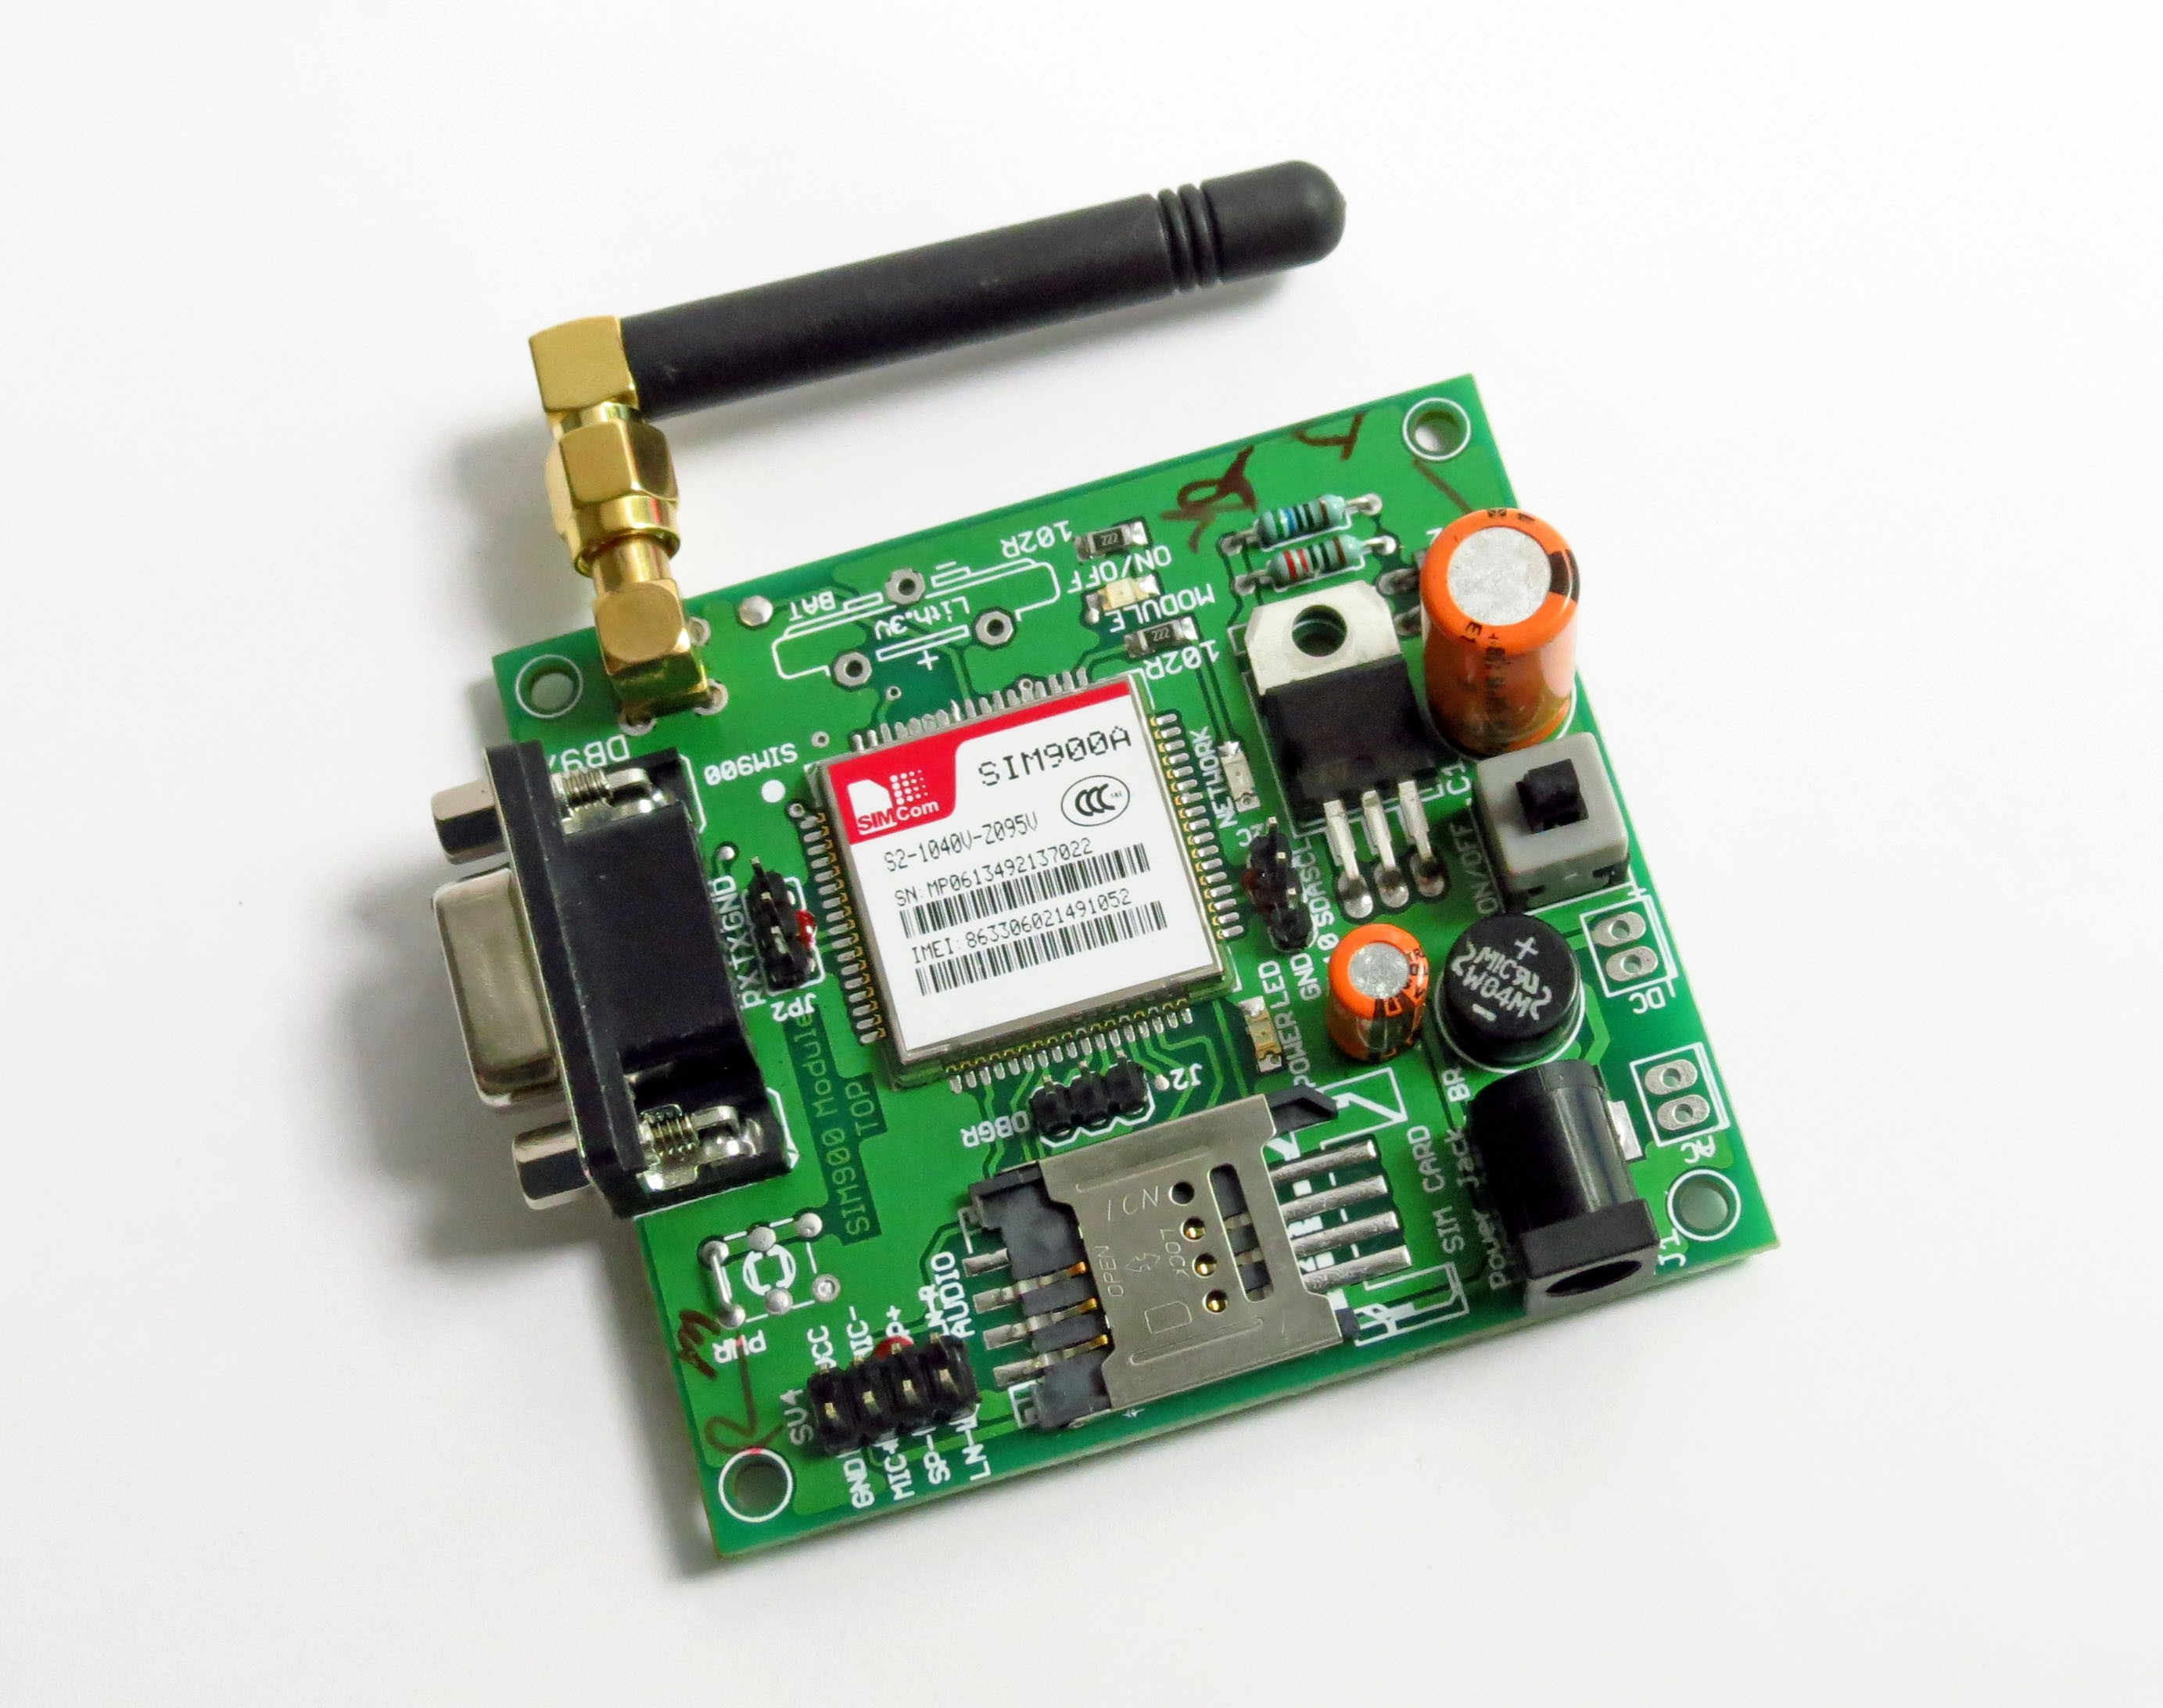
\includegraphics[width=10.0cm]{12.jpg}
					\caption{GSM Module [21]}
				\end{center}
			\end{figure}
			\subsection*{Features}
			\begin{itemize}
				\item Improved spectrum efficiency
				\item International roaming
				\item Compatibility with integrated services digital network (ISDN)
				\item Support for new services.
				\item SIM phonebook management
				\item Fixed dialing number (FDN)
				\item Real time clock with alarm management
				\item High-quality speech
				\item Uses encryption to make phone calls more secure
				\item Short message service (SMS) 
			\end{itemize}
			The security strategies standardized for the GSM system make it the most secure telecommunications standard currently accessible. Although the confidentiality of a call and secrecy of the GSM subscriber is just ensured on the radio channel, this is a major step in achieving end-to- end security.
			\subsection{GSM Architecture}
			A GSM network consists of the following components:
			\begin{itemize}
				
				\item {\bf A Mobile Station}:  It is the mobile phone which consists of the transceiver, the display and the processor and is controlled by a SIM card operating over the network.
				\item {\bf Base Station Subsystem}: It acts as an interface between the mobile station and the network subsystem. It consists of the Base Transceiver Station which contains the radio transceivers and handles the protocols for communication with mobiles. It also consists of the Base Station Controller which controls the Base Transceiver station and acts as a interface between the mobile station and mobile switching centre.
				\item {\bf Network Subsystem}: It provides the basic network connection to the mobile stations. The basic part of the Network Subsystem is the Mobile Service Switching Centre which provides access to different networks like ISDN, PSTN etc. It also consists of the Home Location Register and the Visitor Location Register which provides the call routing and roaming capabilities of GSM. It also contains the Equipment Identity Register which maintains an account of all the mobile equipments wherein each mobile is identified by its own IMEI number. IMEI stands for International Mobile Equipment Identity.
			\end{itemize}
			\subsection{Working of GSM Module:}
			From the below circuit, a GSM modem duly interfaced to the MC through the level shifter IC Max232. The SIM card mounted GSM modem upon receiving digit command by SMS from any cell phone send that data to the MC through serial communication. While the program is executed, the GSM modem receives command ‘STOP’ to develop an output at the MC, the contact point of which are used to disable the ignition switch. The command so sent by the user is based on an intimation received by him through the GSM modem ‘ALERT’ a programmed message only if the input is driven low. The complete operation is displayed over 16×2 LCD display.
			
			
			\section{Motion Sensor }
			PIR sensors allow you to sense motion, almost always used to detect whether a human has moved in or out of the sensors range. They are small, inexpensive, low-power, easy to use and don't wear out. For that reason they are commonly found in appliances and gadgets used in homes or businesses. They are often referred to as PIR, "Passive Infrared", "Pyroelectric", or "IR motion" sensors.
			\begin{figure}[ht!]
				\begin{center}
					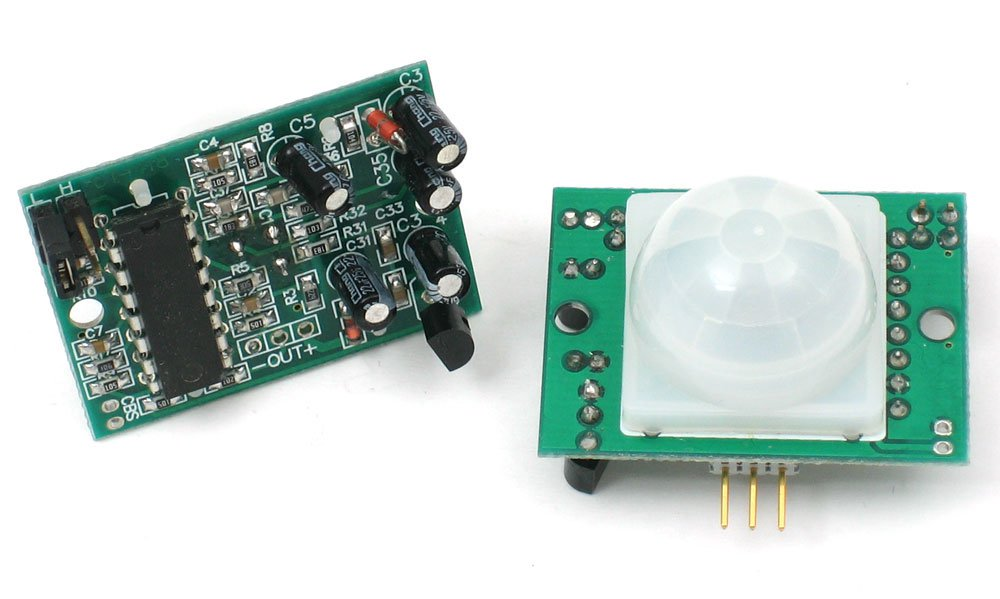
\includegraphics[width=10.0cm]{13.jpg}
					\caption{Motion Sensor [22]}
				\end{center}
			\end{figure}
			For many basic projects or products that need to detect when a person has left or entered the area, or has approached, PIR sensors are great. They are low power and low cost, pretty rugged, have a wide lens range, and are easy to interface with. Note that PIRs won't tell you how many people are around or how close they are to the sensor, the lens is often fixed to a certain sweep and distance (although it can be hacked somewhere) and they are also sometimes set off by housepets. Experimentation is key.
			\begin{figure}[ht!]
				\begin{center}
					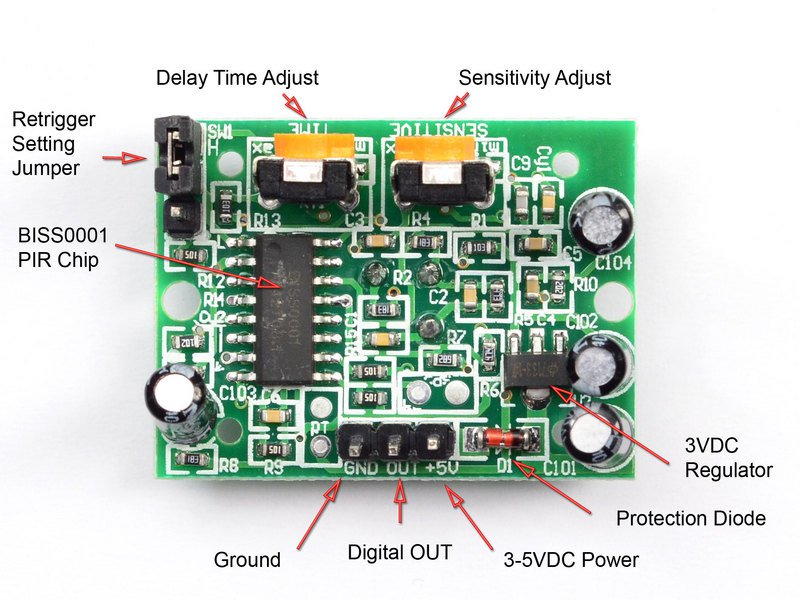
\includegraphics[width=8.0cm]{14.jpg}
					\caption{Motion Sensor [22]}
				\end{center}
			\end{figure}
			\subsection{How PIRs Work}
			PIR sensors are more complicated than many of the other sensors explained in these tutorials (like photocells, FSRs and tilt switches) because there are multiple variables that affect the sensors input and output. To begin explaining how a basic sensor works, we'll use this rather nice diagram
			\begin{figure}[ht!]
				\begin{center}
					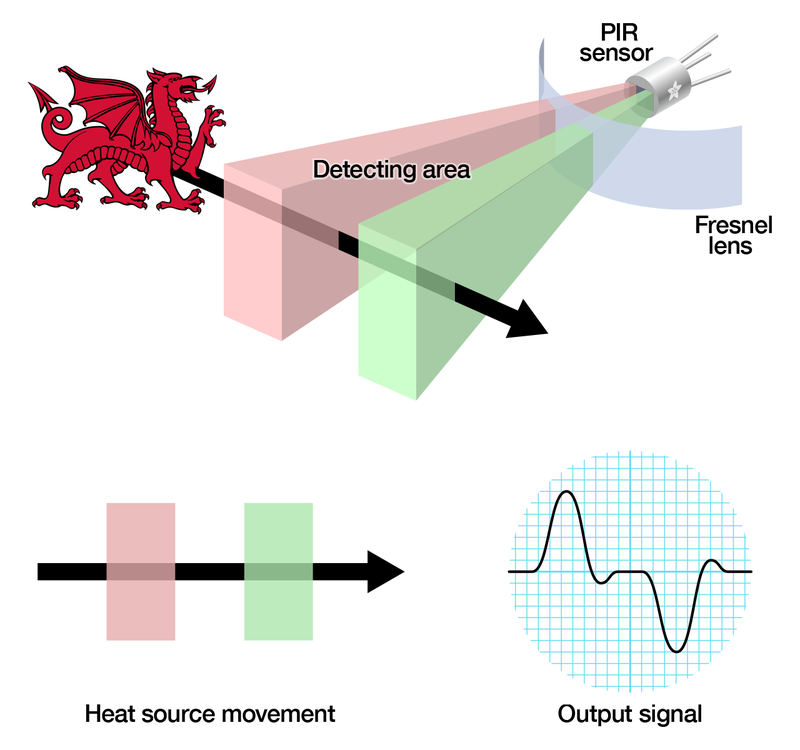
\includegraphics[width=10.0cm]{15.png}
					\caption{Working Animation [22]}
				\end{center}
			\end{figure}
			The PIR sensor itself has two slots in it, each slot is made of a special material that is sensitive to IR. The lens used here is not really doing much and so we see that the two slots can 'see' out past some distance (basically the sensitivity of the sensor). When the sensor is idle, both slots detect the same amount of IR, the ambient amount radiated from the room or walls or outdoors. When a warm body like a human or animal passes by, it first intercepts one half of the PIR sensor, which causes a positive differential change between the two halves. When the warm body leaves the sensing area, the reverse happens, whereby the sensor generates a negative differential change. These change pulses are what is detected.
			
			\section{ESP 8266 Wifi Module }
			The chip first came to the attention of western makers in August 2014 with the ESP-01 module, made by a third-party manufacturer, Ai-Thinker. This small module allows microcontrollers to connect to a Wi-Fi network and make simple TCP/IP connections using Hayes-style commands. However, at the time there was almost no English-language documentation on the chip and the commands it accepted. The very low price and the fact that there were very few external components on the module which suggested that it could eventually be very inexpensive in volume, attracted many hackers to explore the module, chip, and the software on it, as well as to translate the Chinese documentation.
			The ESP8285 is an ESP8266 with 1 MiB of built-in flash, allowing for single-chip devices capable of connecting to Wi-Fi.
			\begin{figure}[ht!]
				\begin{center}
					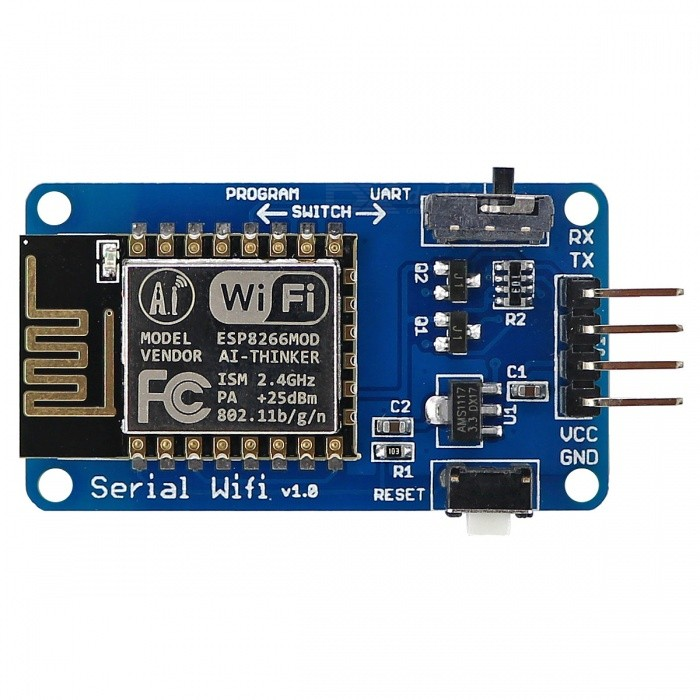
\includegraphics[width=5.0cm]{16.jpg}
					\caption{ESP 8266 Module [25]}
				\end{center}
			\end{figure}
			\subsection*{Features}
			\begin{itemize}
				\item Processor: L106 32-bit RISC microprocessor core based on the Tensilica Xtensa Diamond Standard 106Micro running at 80 MHz
				\item 64 KiB of instruction RAM, 96 KiB of data RAM
				\item External QSPI flash: up to 16 MiB is supported (512 KiB to 4 MiB typically included)
				\item IEEE 802.11 b/g/n Wi-Fi
				\begin{itemize}
					\item Integrated TR switch, balun, LNA, power amplifier and matching network
					\item WEP or WPA/WPA2 authentication, or open networks
				\end{itemize}
				\item 16 GPIO pins
				\item IC (software implementation)
				\item UART on dedicated pins, plus a transmit-only UART can be enabled on GPIO2
				\item 10-bit ADC (successive approximation ADC)
				
			\end{itemize}
			\section{LCD 16X2 Display }
			
			
			We come across LCD displays everywhere around us. Computers, calculators, television sets, mobile phones, digital watches use some kind of display to display the time. An LCD is an electronic display module which uses liquid crystal to produce a visible image. The 16×2 LCD display is a very basic module commonly used in DIYs and circuits. The 16×2 translates o a display 16 characters per line in 2 such lines. In this LCD each character is displayed in a 5×7 pixel matrix.[23]
			\begin{figure}[ht!]
				\begin{center}
					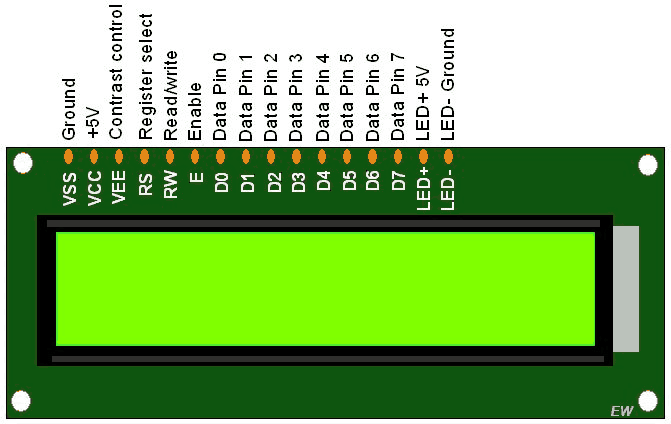
\includegraphics[width=8.0cm]{17.png}
					\caption{ESP 8266 Module [23]}
				\end{center}
			\end{figure}
			\subsection{Displaying Custom Characters on 16X2 LCD}
			Generating custom characters on LCD is not very hard. It requires the knowledge about custom generated random access memory (CG-RAM) of LCD and the LCD chip controller. Most LCDs contain Hitachi HD4478 controller. CG-RAM is the main component in making custom characters. It stores the custom characters once declared in the code. CG-RAM size is 64 byte providing the option of creating eight characters at a time. Each character is eight byte in size.
			CG-RAM address starts from 0x40(Hexadecimal) or 64 in decimal. We can generate custom characters at these addresses. Once we generate our characters at these addresses, now we can print them on the LCD at any time by just sending simple commands to the LCD. Character addresses and printing commands are below
			\section*{RS(Register select)}
			A 16X2 LCD has two registers, namely, command and data. The register select is used to switch from one register to other. RS=0 for command register, whereas RS=1 for data register.
			
			\section*{RS(Register select)}
			The command register stores the command instructions given to the LCD. A command is an instruction given to LCD to do a predefined task like initializing it, clearing its screen, setting the cursor position, controlling display etc. Processing for commands happen in the command register.
			\section*{RS(Register select)}
			The data register stores the data to be displayed on the LCD. The data is the ASCII value of the character to be displayed on the LCD. When we send data to LCD it goes to the data register and is processed there. When RS=1, data register is selected.
			
			
			
			\newpage
			\subsection{PIN Discription}
			\begin{figure}[ht!]
				\begin{center}
					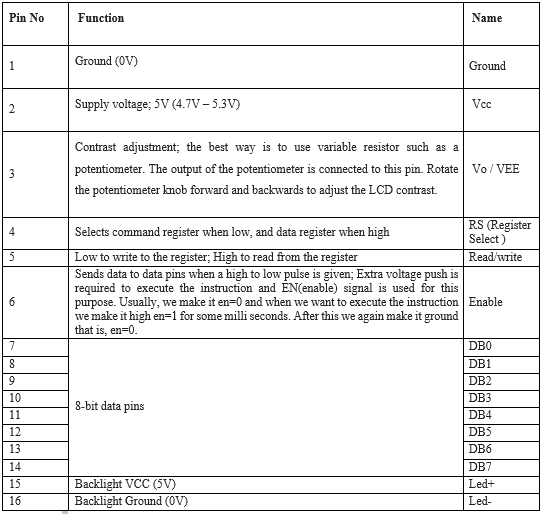
\includegraphics[width=10.0cm]{18.png}
				\end{center}
			\end{figure}
			
			\begin{table}[!ht]
				
				\caption{PIN Discription of LCD [23]}
			\end{table}
			
			
			
			\section{Webcam }
			A webcam is a video camera that feeds or streams its image in real time to or through a computer to a computer network. When "captured" by the computer, the video stream may be saved, viewed or sent on to other networks via systems such as the internet, and emailed as an attachment. When sent to a remote location, the video stream may be saved, viewed or on sent there. Unlike an IP camera (which connects using Ethernet or Wi-Fi), a webcam is generally connected by a USB cable, or similar cable, or built into computer hardware, such as laptops.
			\begin{figure}[ht!]
				\begin{center}
					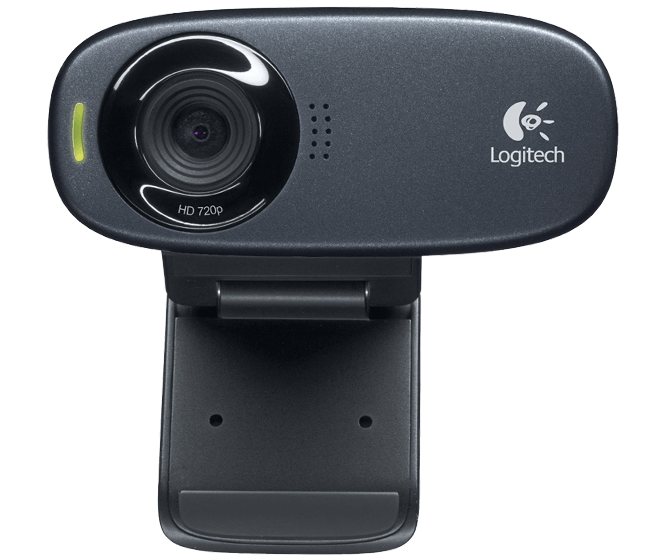
\includegraphics[width=4.0cm]{19.png}
					\caption{Webcam [24]}
				\end{center}
			\end{figure}
			
			The term "webcam" (a clipped compound) may also be used in its original sense of a video camera connected to the Web continuously for an indefinite time, rather than for a particular session, generally supplying a view for anyone who visits its web page over the Internet. Some of them, for example, those used as online traffic cameras, are expensive, rugged professional video cameras.
			
			\section{Basic Electronics components }
			An electronic component is any basic discrete device or physical entity in an electronic system used to affect electrons or their associated fields.
			\begin{figure}[ht!]
				\begin{center}
					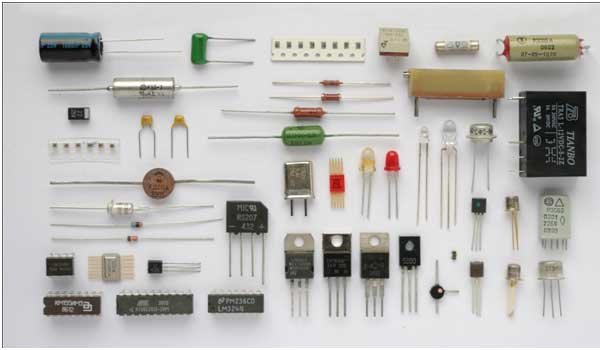
\includegraphics[width=12.0cm]{20.jpg}
					\caption{Basic Electronics Components}
				\end{center}
			\end{figure}
			\chapter{Design of PCB Layout }
			\section{Simulation using proteus sesign suite}
			In this of the project we are purforming simulation process using proteus design suite in this stage of ptoject we are simulating only half portion of the circuit.
			Following is the screenshot of designed circuit.
			\begin{figure}[ht!]
				\begin{center}
					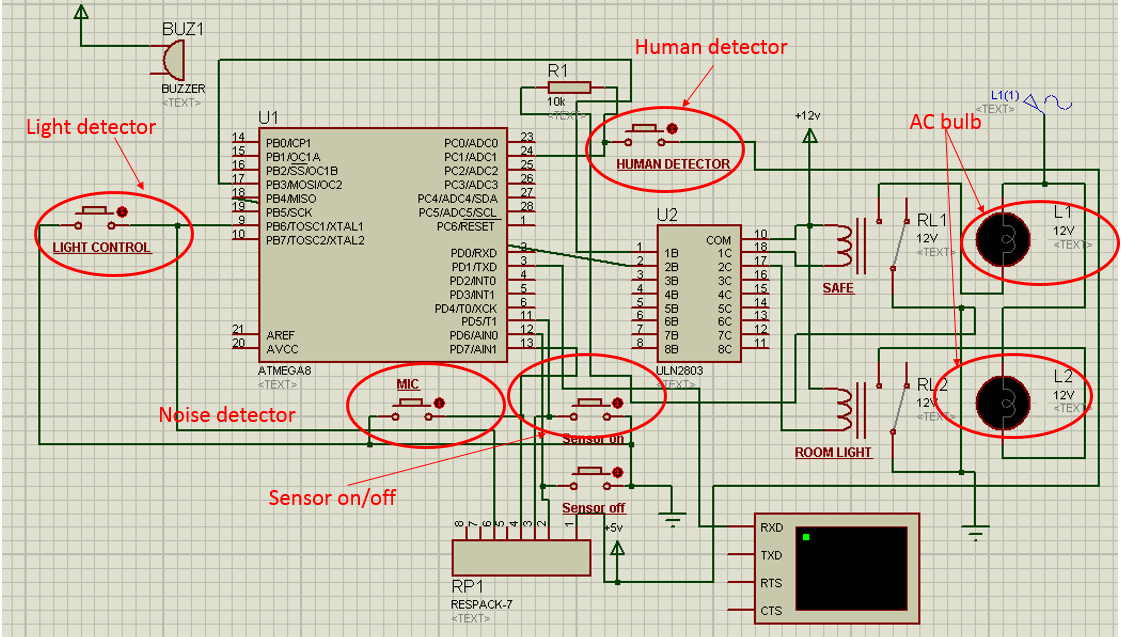
\includegraphics[width=17.0cm]{f4.png}
					\caption{Simulation of circuit}
				\end{center}
			\end{figure}
			\newpage
			\section{PCB Layout}
			\begin{figure}[ht!]
				\begin{center}
					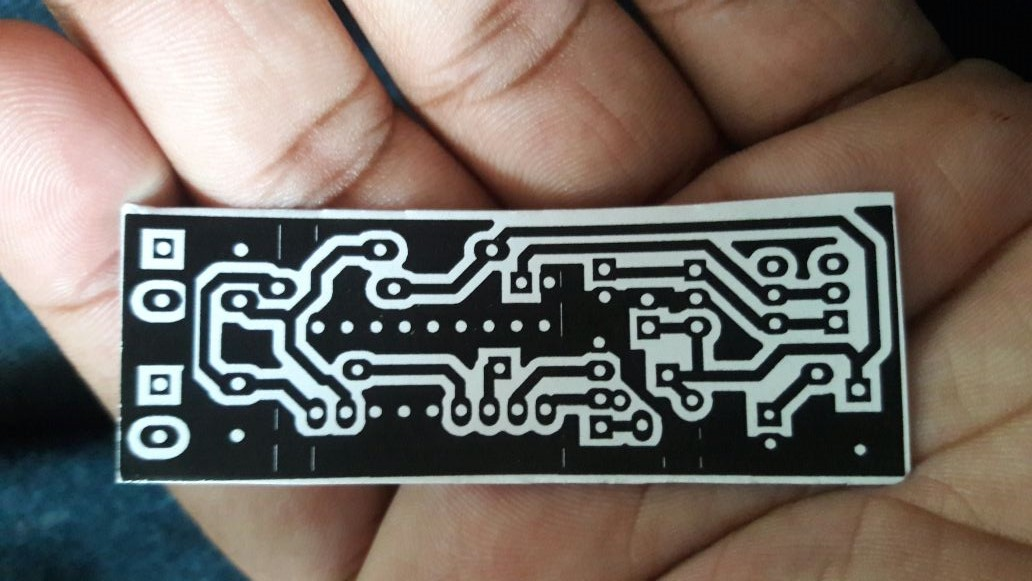
\includegraphics[width=17.0cm]{p1.jpeg}
					\caption{Layout of transmitter section }
				\end{center}
			\end{figure}
			\begin{figure}[ht!]
				\begin{center}
					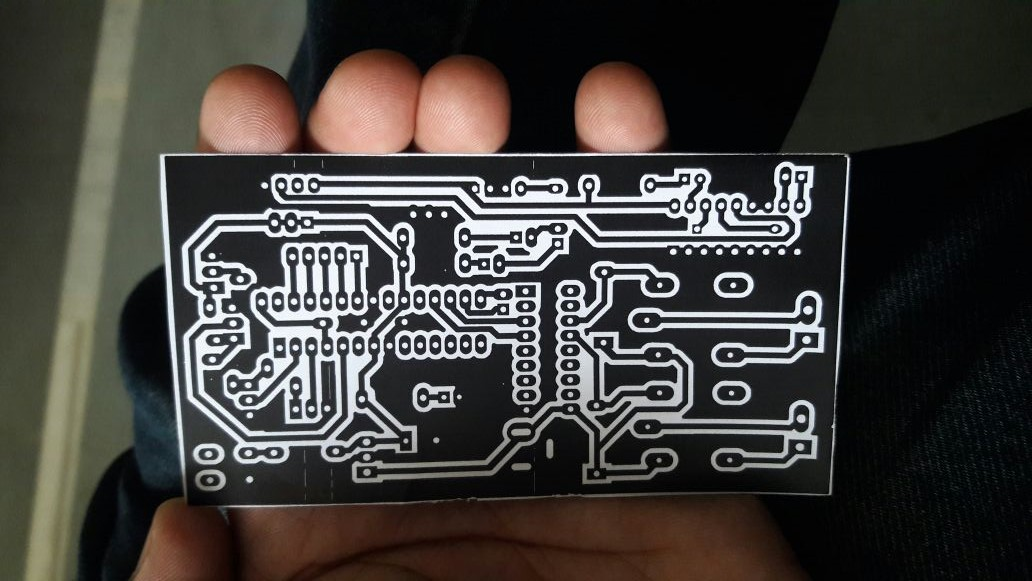
\includegraphics[width=17.0cm]{p2.jpeg}
					\caption{Layout of ATmega 8 controller section }
				\end{center}
			\end{figure}
			
			\section{Hardware Components and Configuration of the Proposed System}
			The components of the proposed digital door lock system and their functions are discussed before. A microcontroller is required to control the door lock and a ESP866 module is used for communicating with the mobile device. An ultrasonic sensor is required to recognize a nearby user; an impact vibration sensor is also required. OpenWrt is used as the operating system of the system; the program to operate the controller is written in C; PHP and HTML are used for the web programming and database management, respectively; and UHTTP is used for the web server instead of Apache.
			
			Besides, various sensors for proximity and intrusion detection are connected to the system. A camera sensor for photographing an image of invalid users is installed, an impact sensor is attached for detecting a physical shock by an invalid user, and an ultrasonic sensor is attached to recognize the proximity of valid users. 
			\begin{figure}[ht!]
				\begin{center}
					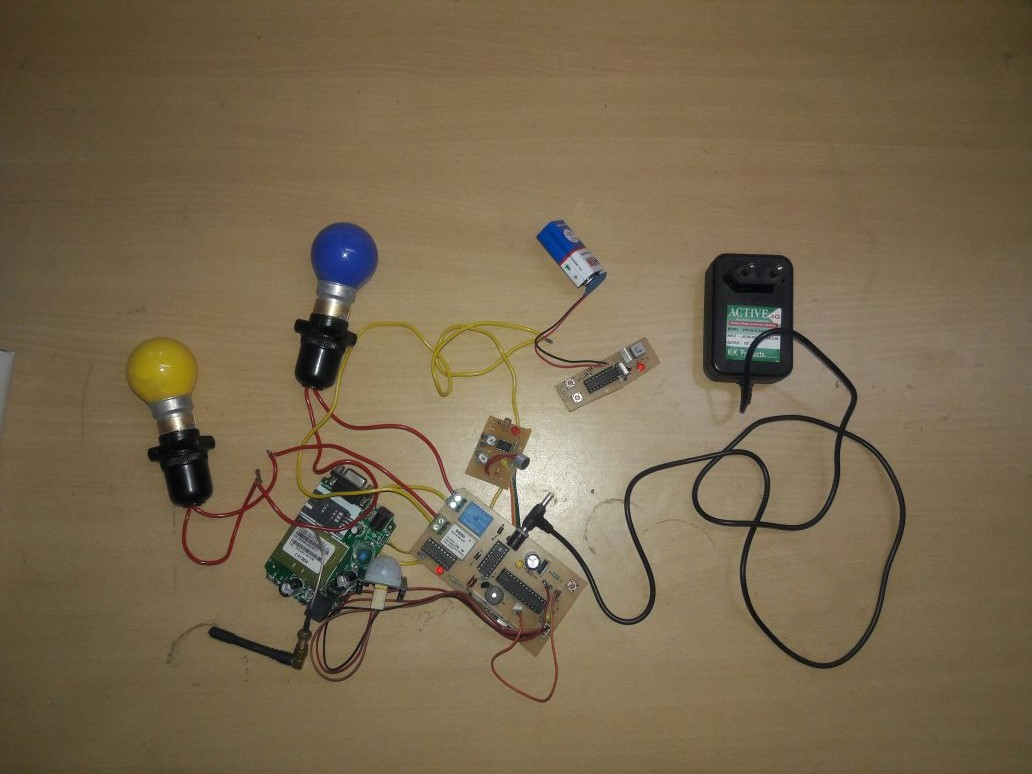
\includegraphics[width=17.0cm]{f7.jpeg}
					\caption{Hardware }
				\end{center}
			\end{figure}
			\section{Programing}
			Following figure shows that programing logic of proposed design which is done with the help of ATmal studio version 5.1 using c.
			\newpage
			\begin{figure}[ht!]
				\begin{left}
					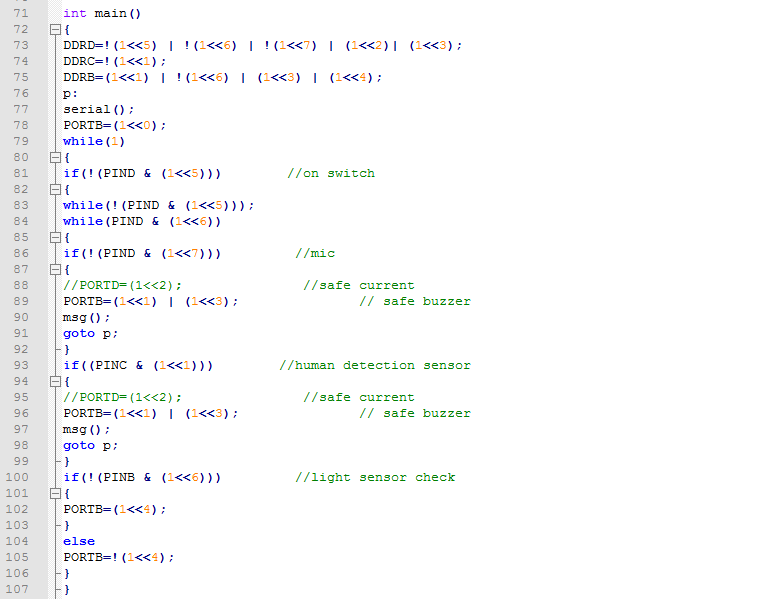
\includegraphics[width=15.0cm]{p5.png}
					\caption{Coding of desired hardware }
				\end{left}
			\end{figure}
			\begin{figure}[ht!]
				\begin{left}
					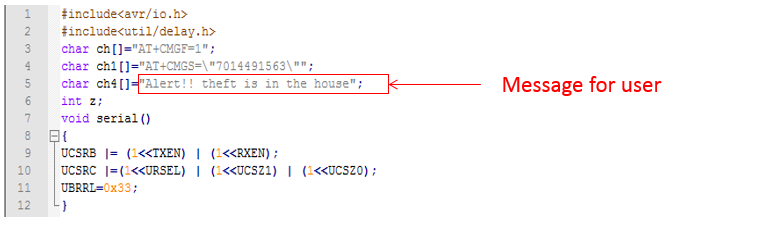
\includegraphics[width=15.0cm]{p7.png}
					\caption{Coading for desired message }
				\end{left}
			\end{figure}
			\chapter{Prototype of Project}
			\section{Design}
			There are two sections in our task. They are the security framework and the heap controlling framework. In the security framework we utilize a few sensors, for example, Biometric sensor, Webcam, movement sensor. In the heap controlling framework we utilize hand-off to on or off the heap. We have utilized GSM module to send message to a supporter distinguishing proof number about security reason. We have additionally utilized this GSM module to control stack from remote region.
			\subsection{Control Unit }
			The control unit (Fig.6.1)  was housed in a 20 cm x 30 cm x 5 cm Plastic box . The user interface was made possible by making LCD and fingerprint slots on the box . Different slots were given for the GSM antenna, ESP8266, the motor interface terminals and the DC input power supply. The unit had a removable lid at back for maintenance purposes.
			\begin{figure}[ht!]
				\begin{center}
					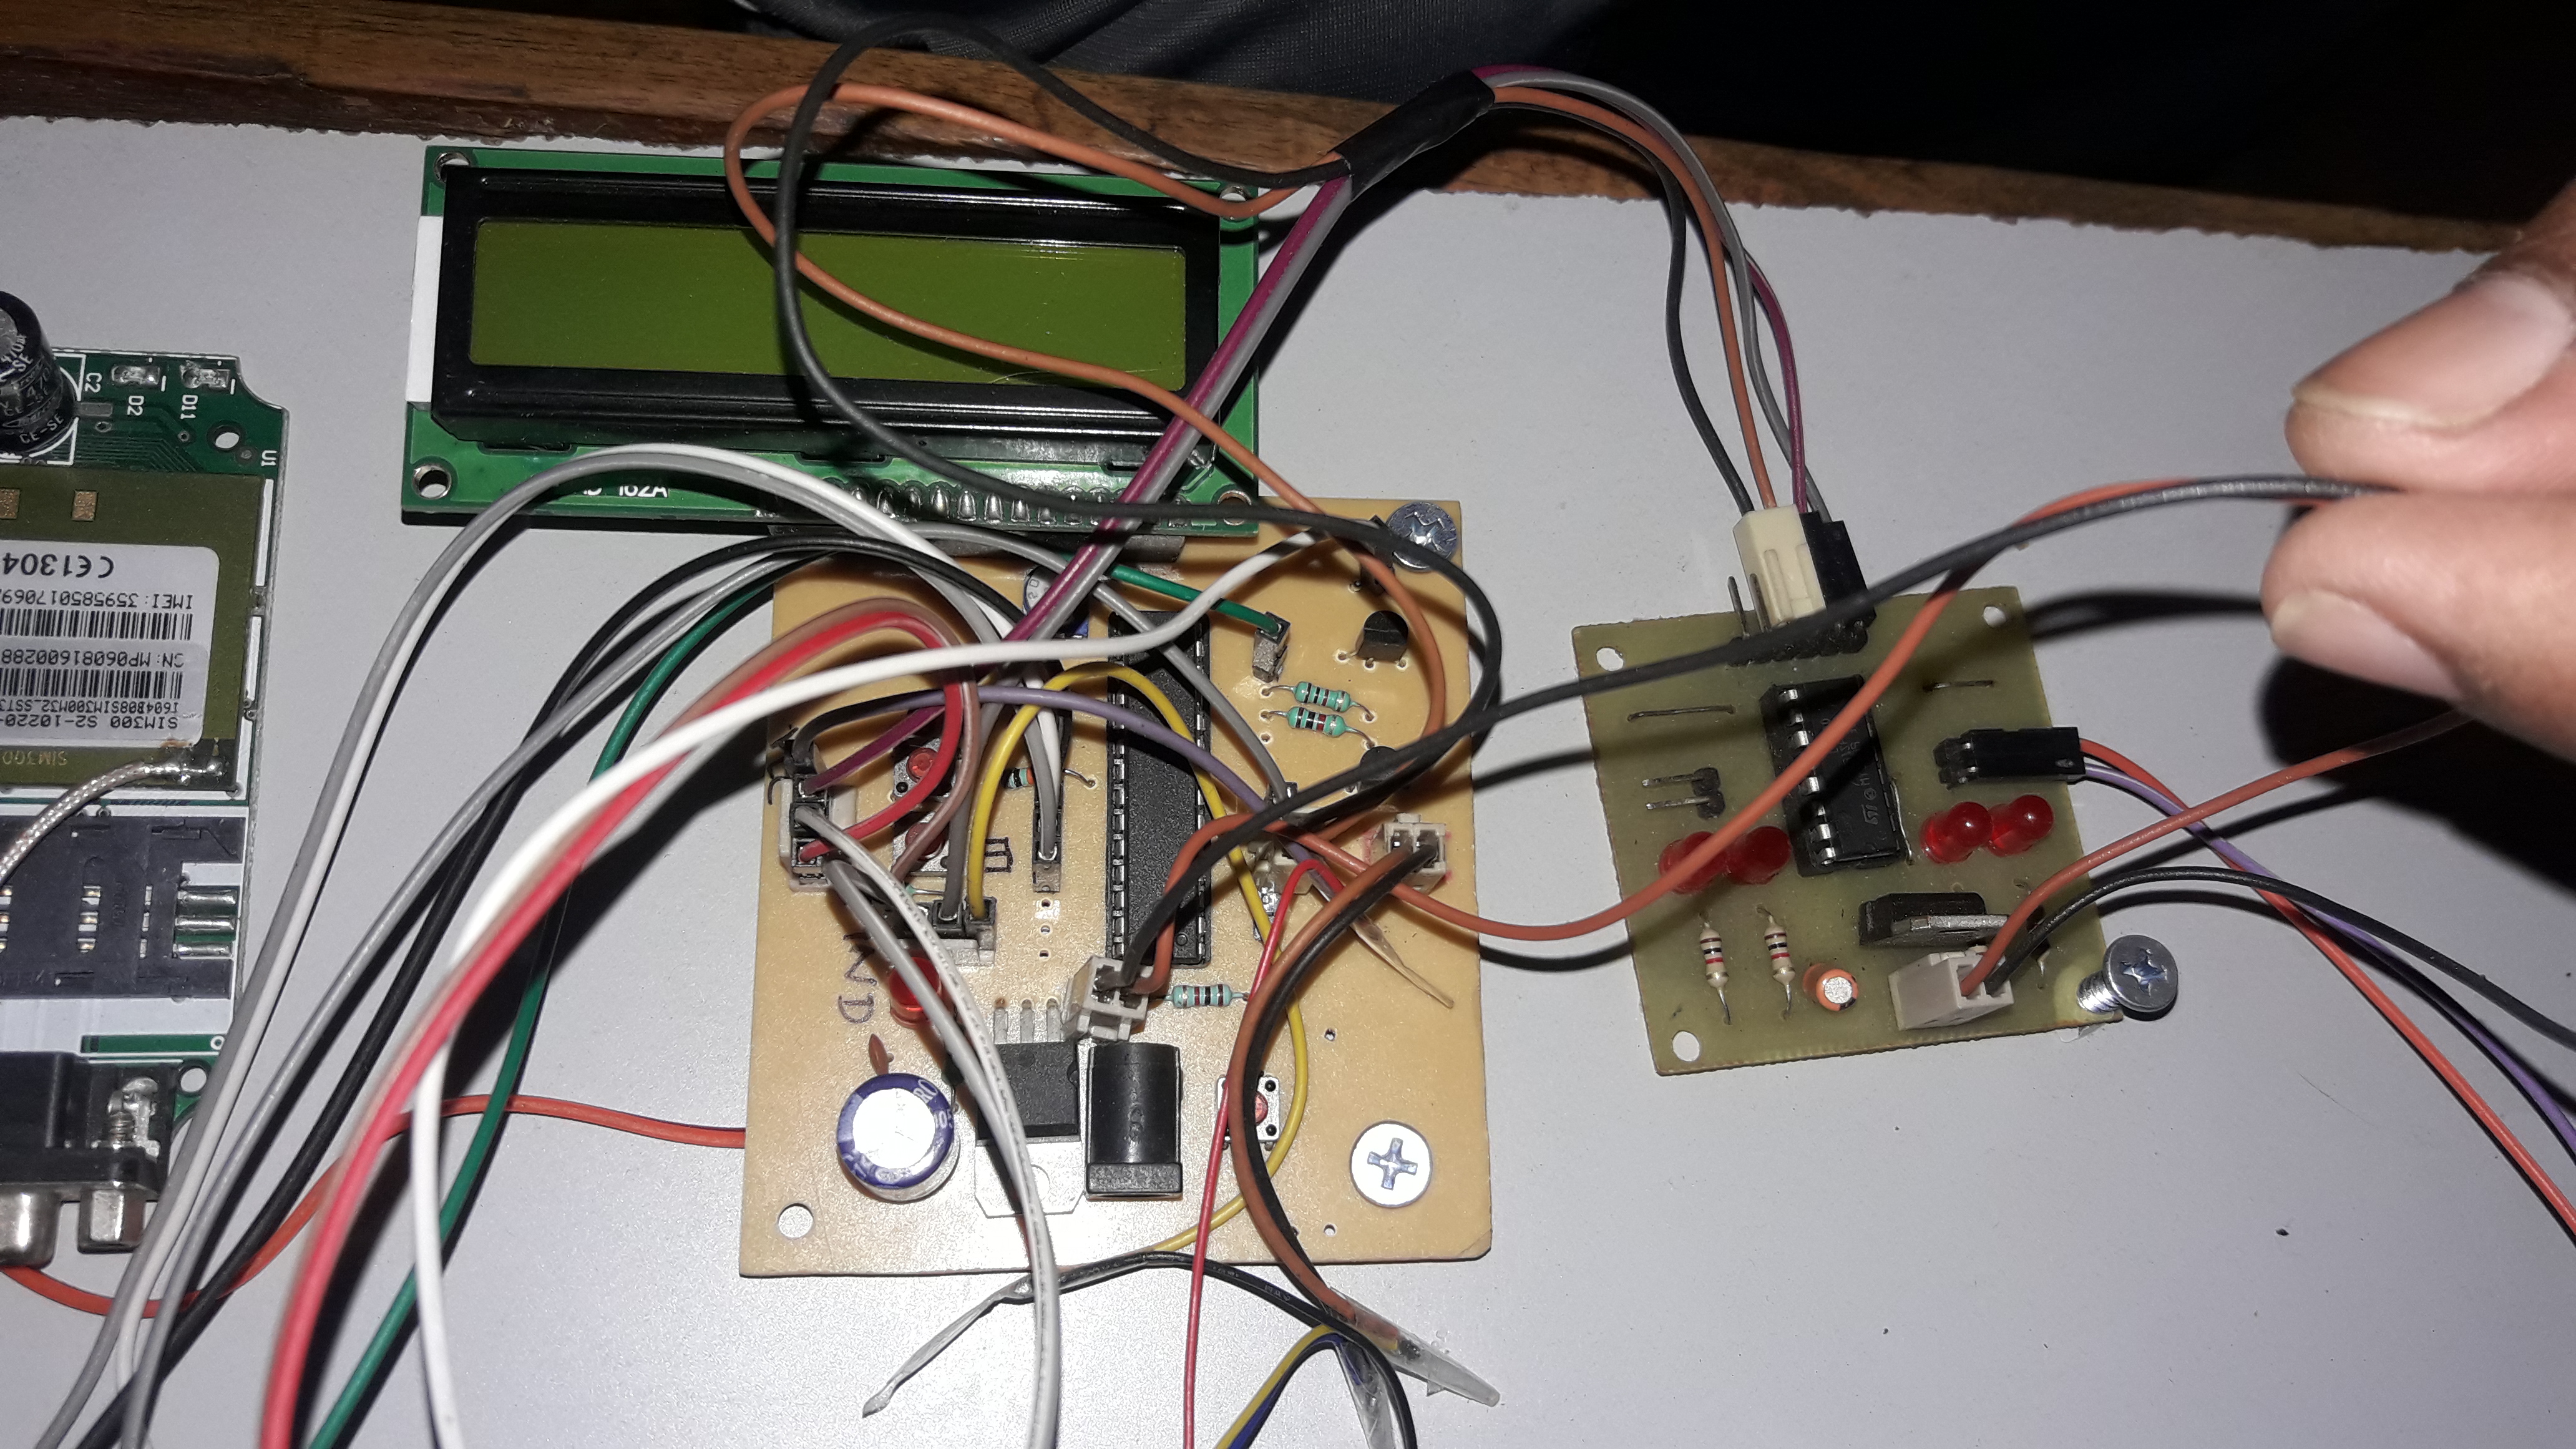
\includegraphics[width=14.0cm]{cont.jpg}
					\caption{Control Unit }
				\end{center}
			\end{figure}
			\subsection{Demonstration Model}
			For the purpose of a real-time demonstration of locking and unlocking of door lock we constructed a scaled model of a house with three walls and roof (Fig 6.2). The door was made by a DVD drive sliding portion for demonstration which is coupled by a DC Motor. The dimension of the demo house was 36 cm x 20 cm x 20 cm.      In this   demo house we have installed our GSM section in back side of the demo house and this can be installed anywhere user wants to install.\\
			\begin{figure}[ht!]
				\begin{center}
					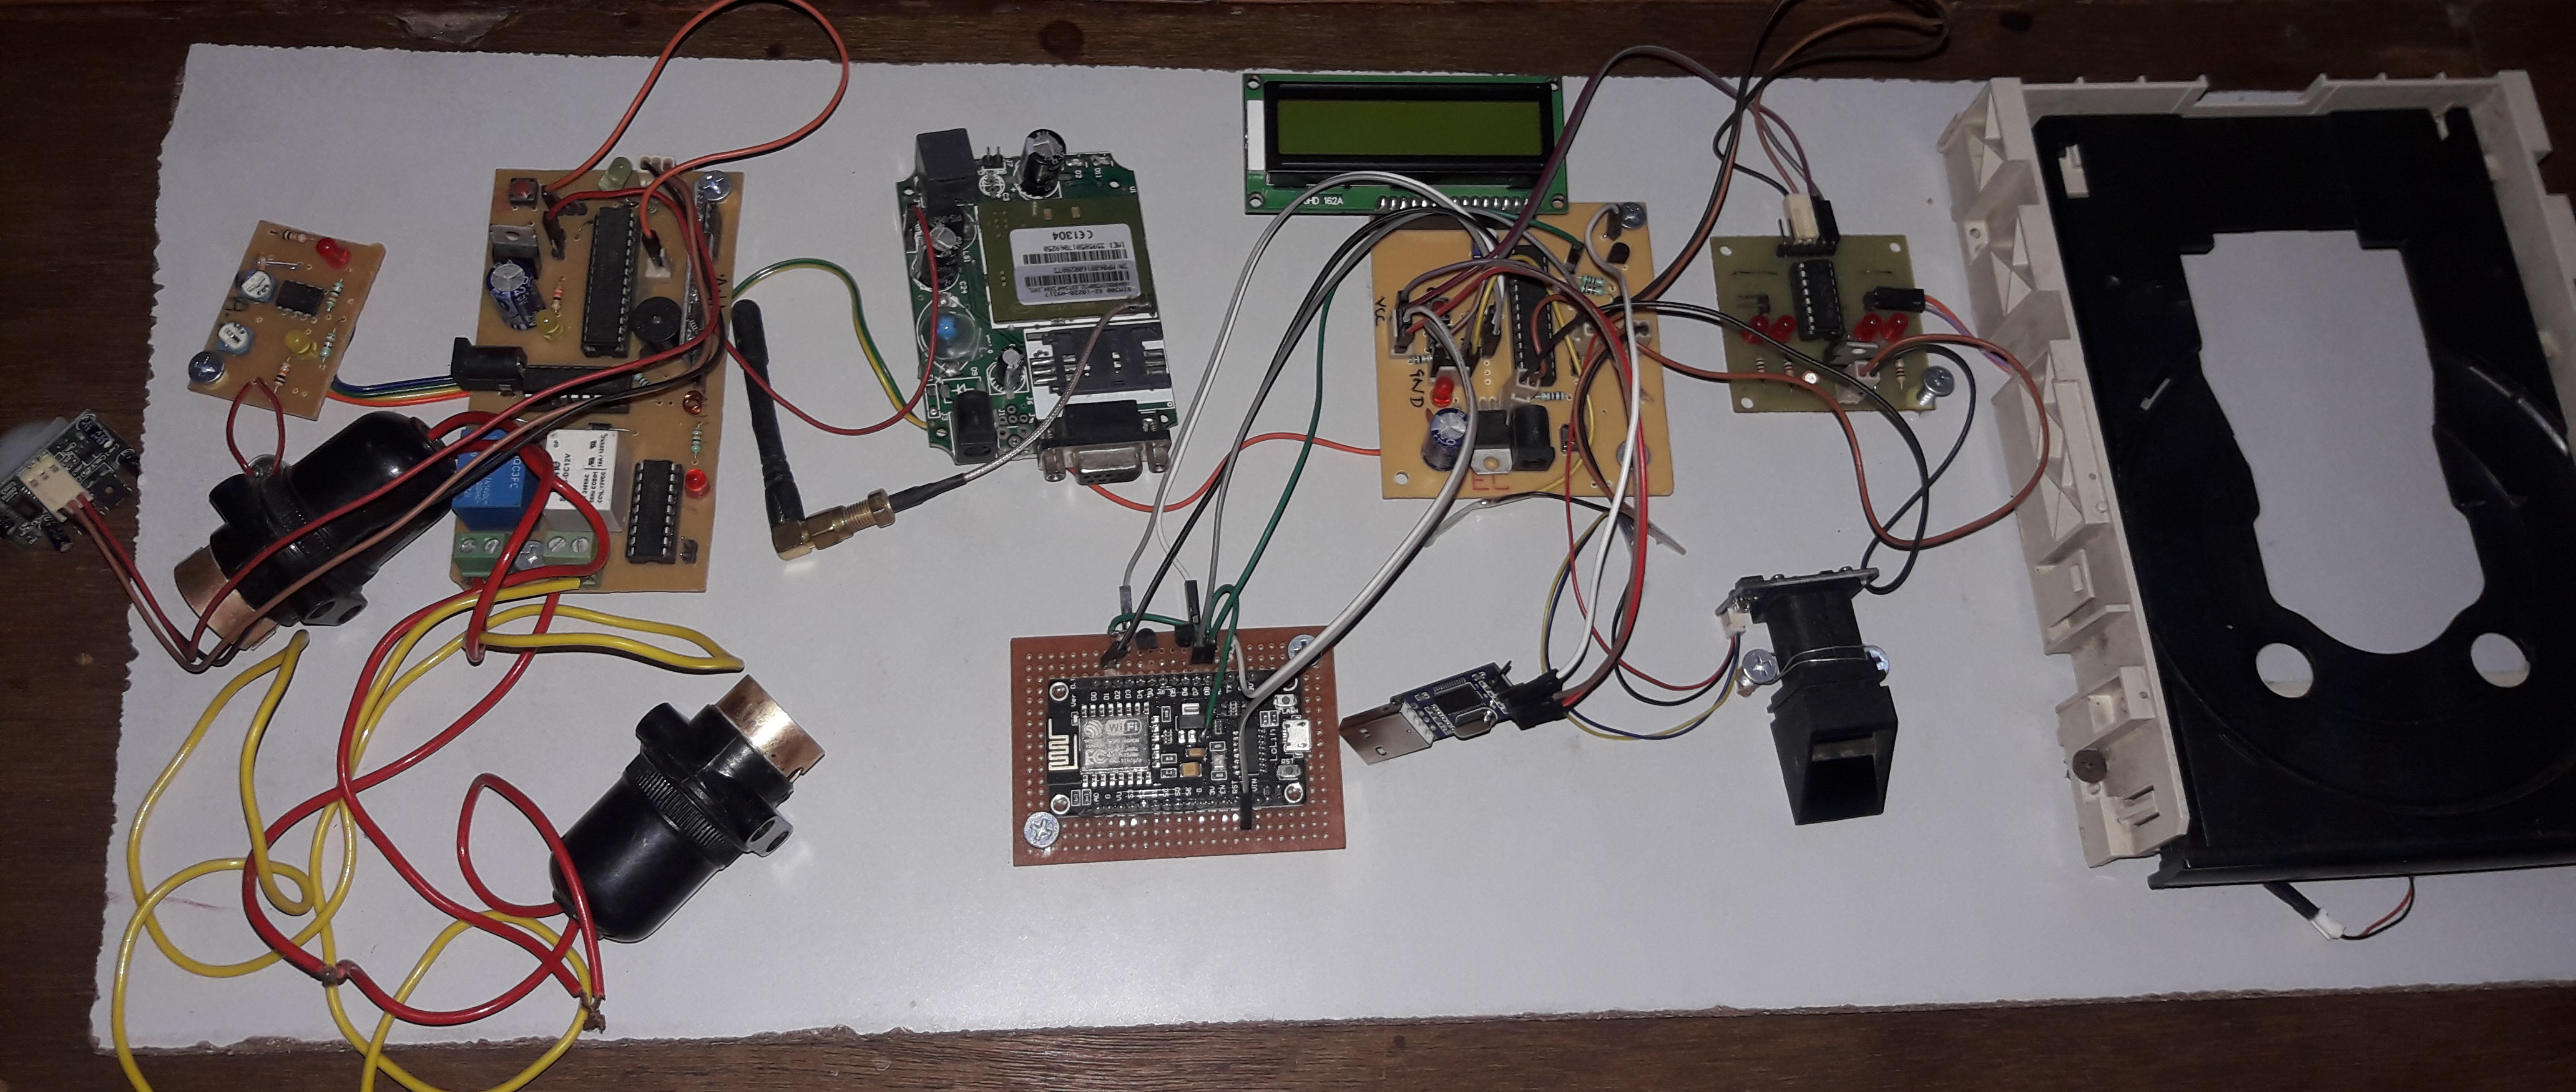
\includegraphics[width=15.0cm]{cont1.jpg}
					\caption{Demonstration Model }
				\end{center}
			\end{figure}
			\subsection{IOT section}
			In this section we have used ESP8366 module for access door lock control from internet. With the help of Blynk android app we have interfaced our ESP8266 module and with this app we can now control the door for valid and invalid user. All the notifications like who entered can be seen by this app. To access the internet through the ESP8266 Module we are using our android phone Samsung J7.
			\begin{figure}[ht!]
				\begin{center}
					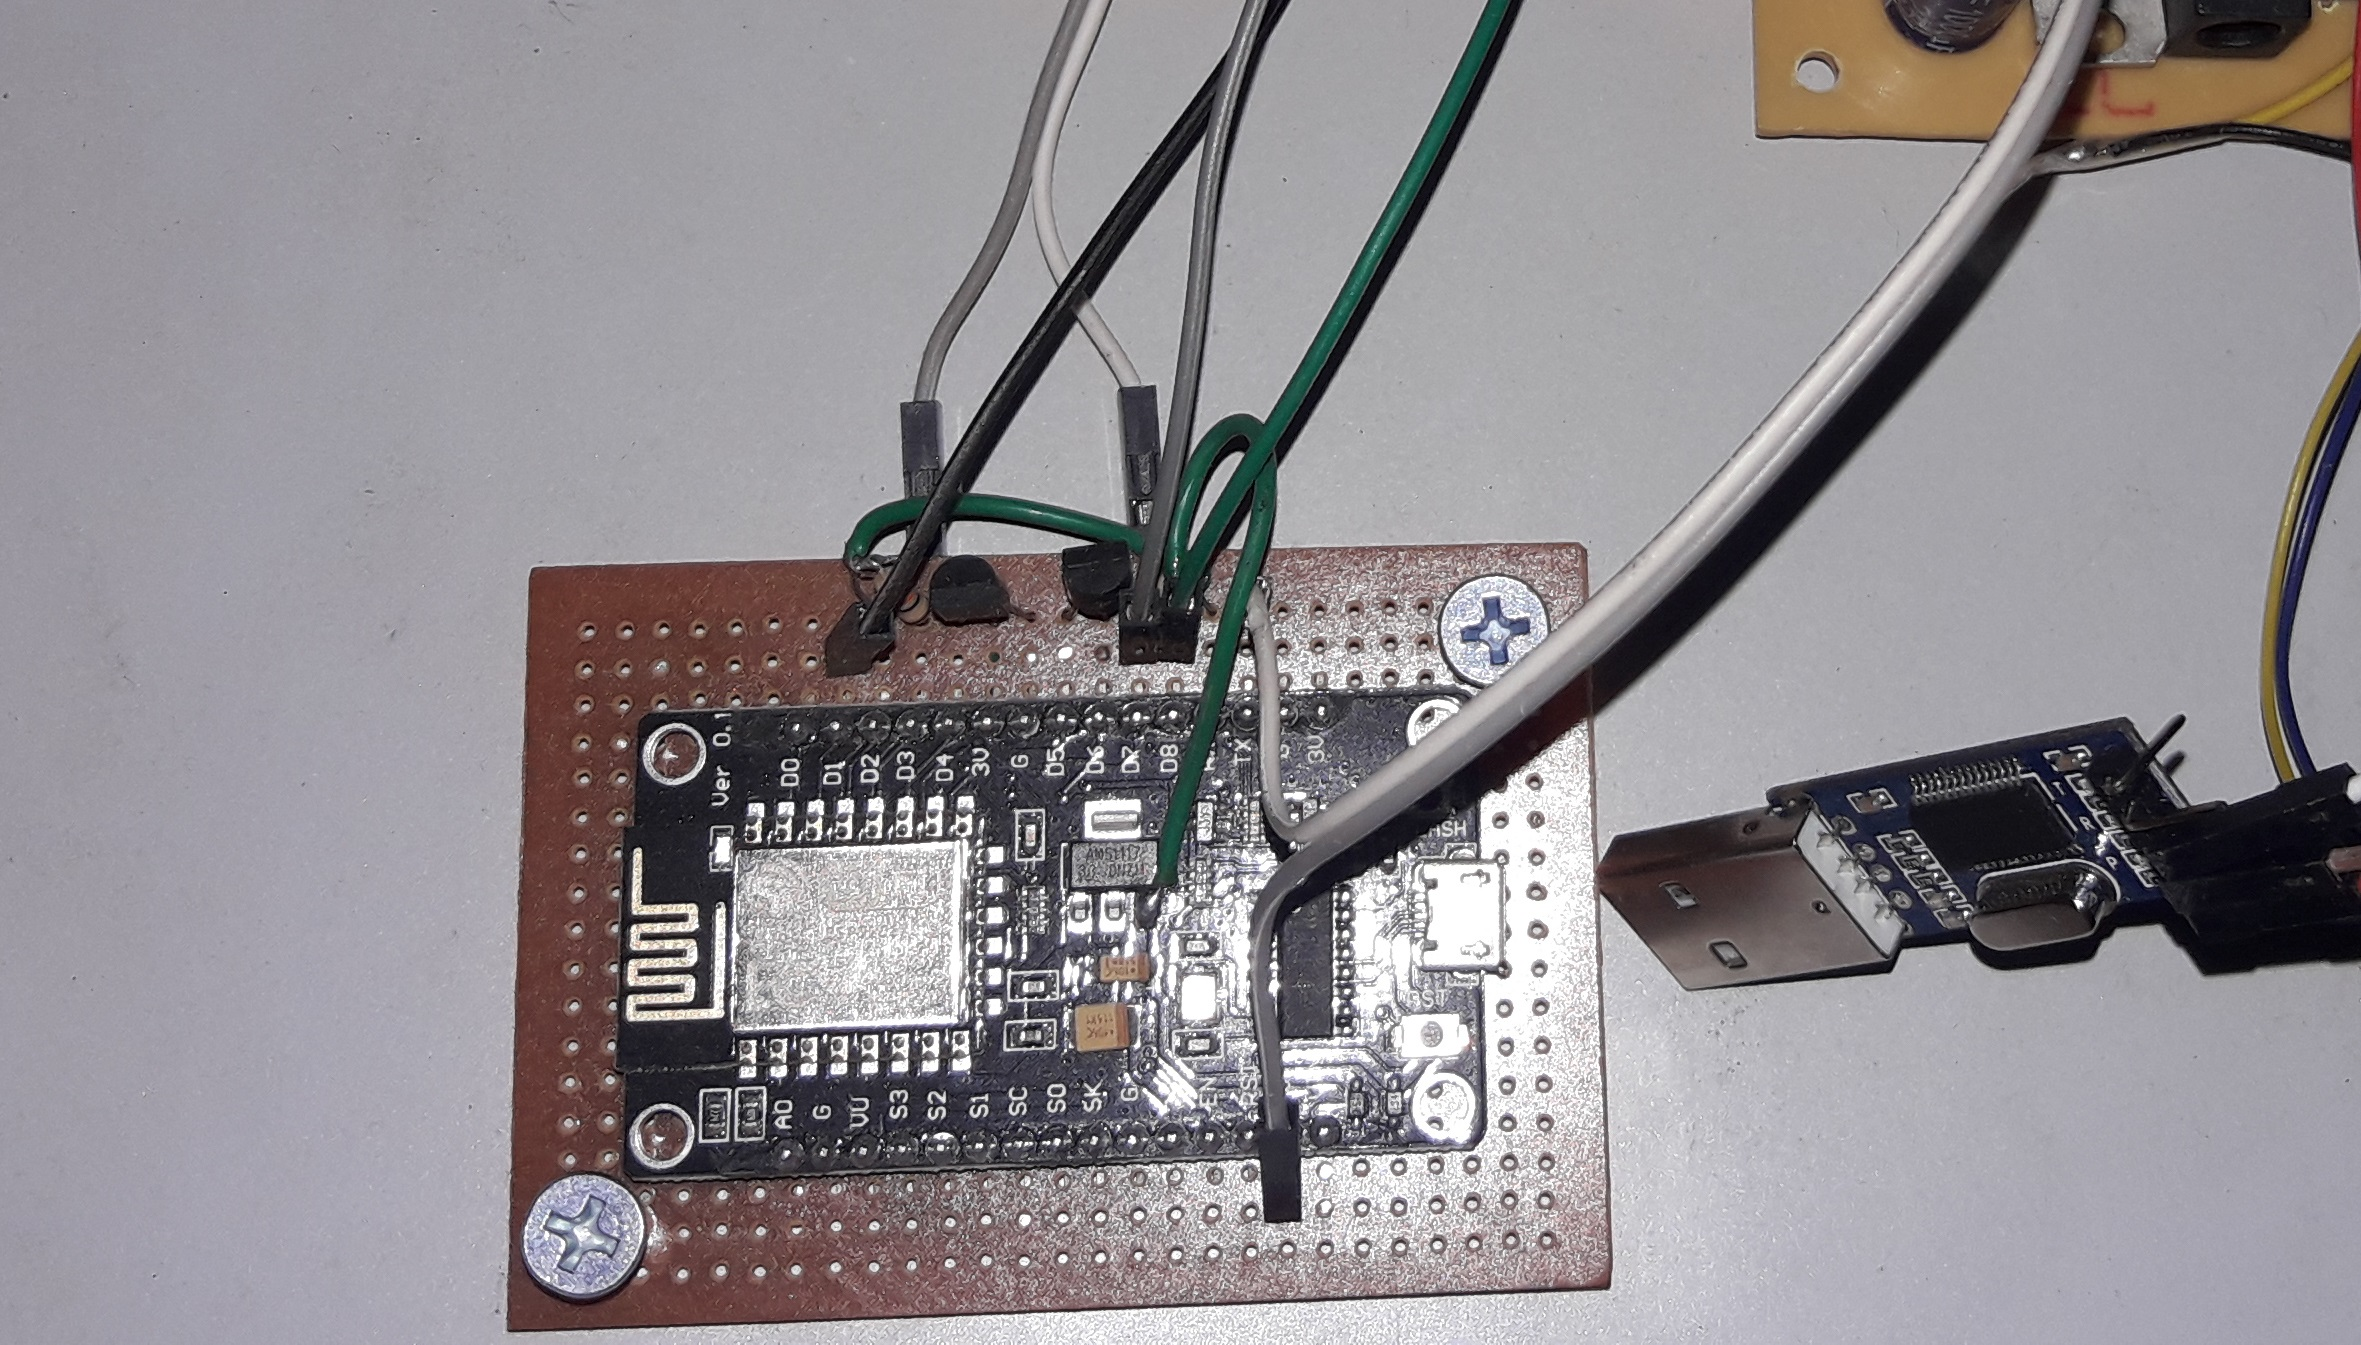
\includegraphics[width=7.0cm]{count2.jpg}
					\caption{IoT Section }
				\end{center}
			\end{figure}
			\subsection{GSM module section}
			In This section of the project we are using a GSM module to communicate with admin during emergencies through message in this section we have also used PIR sensor as Motion detector or Light detector and also used a noise detector.
			\begin{figure}[ht!]
				\begin{center}
					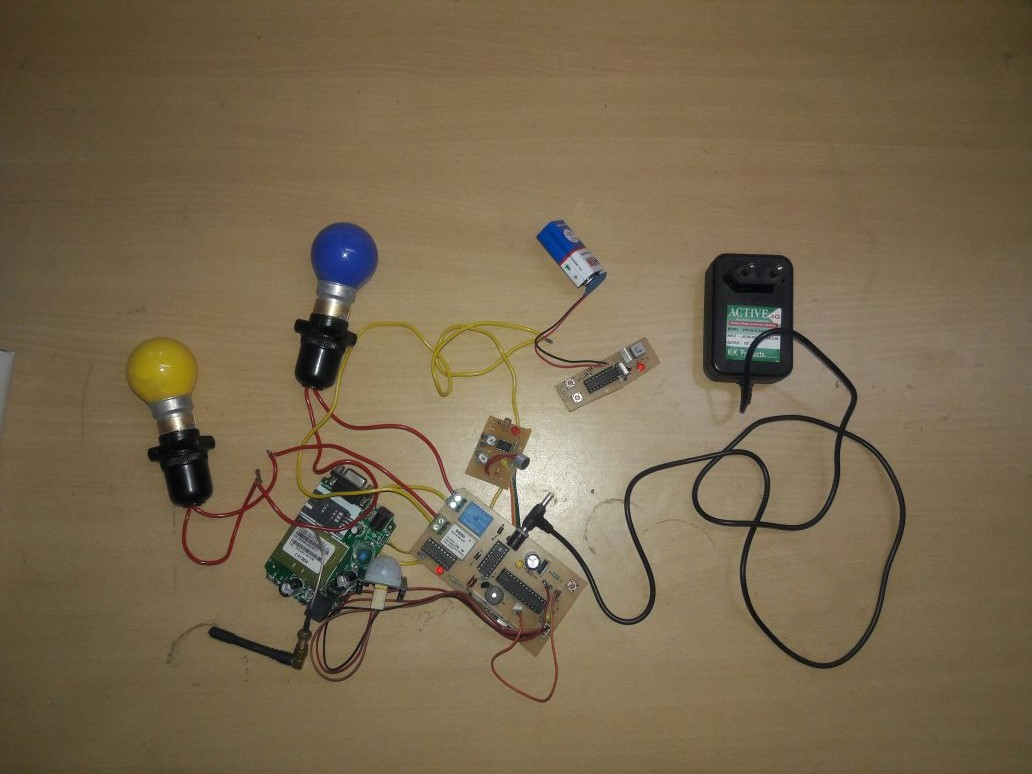
\includegraphics[width=10.0cm]{f7.jpeg}
					\caption{GSM and Theft Detection Section }
				\end{center}
			\end{figure}
			
			\chapter{Project Evaluations }
			\section{Results and Analysis}
			The prototype of the IOT and GSM Based Smart Security System was designed and implemented successfully. A detailed analysis was done on the working and stability of the system. Our findings were:
			\subsection{Analysis for Valid User}
			For the initial startup of the system it took 10 second to start. After the fingerprint verification it took 2 second to unlock the door (fig. 8) and notify the user with its name on blynk app door automatically closed after 10 second.
			\begin{figure}[ht!]
				\begin{center}
					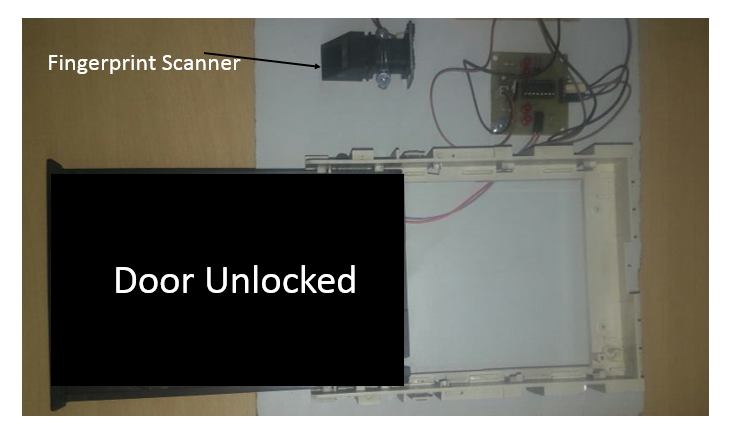
\includegraphics[width=10.0cm]{ff.png}
					\caption{Door Unlocked During Valid Users }
				\end{center}
			\end{figure}
			\subsection{Analysis for Invalid User}
			In this analysis of the project we have divided it into two case one for if user in known and another one is for if user is unknown.
			\subsection*{Case 1 (Invalid user is known) :}
			In this case of the project it took 5 second to notify the admin with captured picture of the user with the help of blynk app  and MATLAB process  and validity alert will be set to the HIGH. Now admin will take the decision that user is valid or not and if user press the valid user button then it will take 2 second to unlock the door. 
			\subsection*{Case 1 (Invalid user is Unknown) :}
			In this case of the project it will take 2 second to notify the admin with the captured image and after pressing invalid user button on the blynk app door will be remain locked and no one can enter in the house.
			\begin{figure}[ht!]
				\begin{center}
					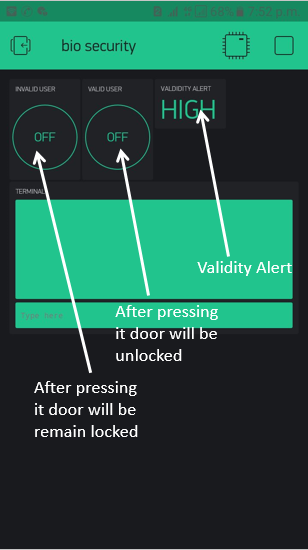
\includegraphics[width=7.0cm]{ff2.png}
					\caption{Blynk App Notification During Both These Cases}
				\end{center}
			\end{figure}
			\\
			\\
			\\
			During both these cases webcam will record video continuously which can be store and seen for further use and all the logs with the captured picture can also be saved for later use. Captured images and recorded video can be send to the remote location by an email attachment.
			\begin{figure}[ht!]
				\begin{center}
					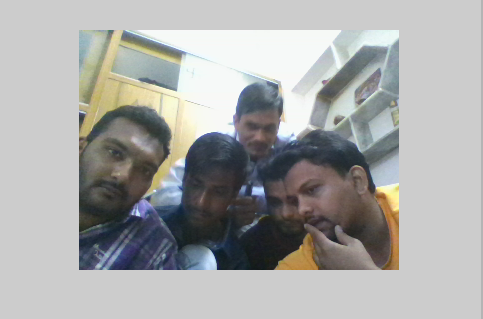
\includegraphics[width=10.0cm]{ff1.png}
					\caption{Capture image with webcam during analysis of Invalid user}
				\end{center}
			\end{figure}
			\subsection{Analysis of Motion or Light Detection unit}
			In this section of the project we have used GSM module to notify the with a alert message if any one entered in the house without permission and it will take 10 second to deliver message to user. Here PIR sensor is used as motion detector or light detector and we have also used noise detector. 
			\begin{figure}[ht!]
				\begin{center}
					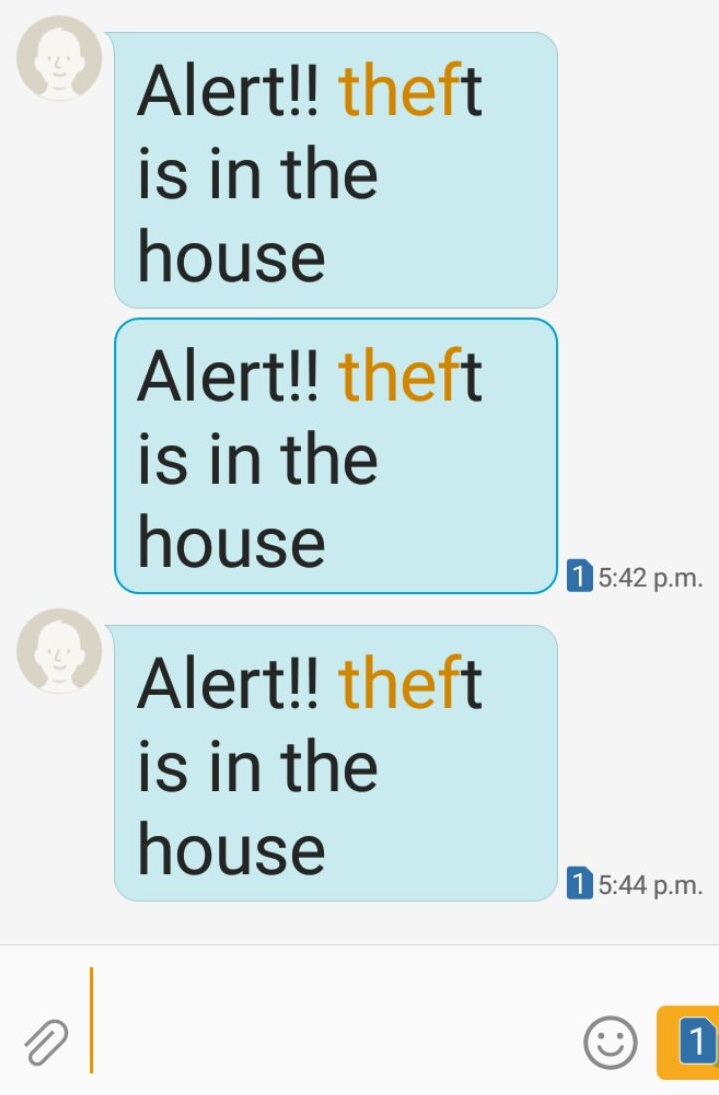
\includegraphics[width=5.0cm]{p3.jpeg}
					\caption{Alert Message}
				\end{center}
			\end{figure}
			\\
			The ‘Capture Log (Intrusion Record)’ menu is for querying intrusion information, such as an invader’s image taken by the controller when a password input error occurs. When an access request is generated by a valid visitor who does not possess the key, the ‘Request’ menu allows the user to check the image of the requester and open the door. The ‘Remote opening’ menu allows for remote door operation. The ‘Option’ menu allows for password management and ‘Bluetooth synchronization (Master mode)’ menu is a setting menu for automatic opening when approaching the door lock. Figure 6 shows the application cases for remote controls. The left side of the top of the figure is the main menu of the App, the right of the top shows the Bluetooth setup button for proximity open and a keypad for the remote open. The left of the bottom of the figure shows a list of the image information that has been captured by physical shock and the input mistake of password. And the right of the bottom shows an image of the item in the list.
			\subsection{Trials}
			An assortment of trials was finished with various cases. A geographic zone with great GSM gathering brought about the conveyance of the notification message in no time flat. It was likewise noticed that the devoted power supply helped the framework to give a fluctuation-free benefit.
			\chapter{Future Scope}
			\section{Conclusion}
			The IoT and GSM based Smart Security System was planned and actualized effectively. On premise of point by point examination and trials, we could infer that the framework was steady and can be a rising item in the field of security frameworks for both private and business applications. We recommend the accompanying changes later on improvement of framework:-
			\begin{itemize}
				\item  Incorporating with 3D holographic password input console.
				\item  Integrating with multiple locks on multiple doors inside a facility.
			\end{itemize}
			The GSM and IOT based smart security system has been designed and tested with the mobile
			network. The user can get alerts anywhere through the GSM technology thus making the
			system location independent. A flexible way to control and explore the services of the mobile,
			AT commands is used in the system. The communication of home is only through the SMS
			which has been tested with the mobile networks and is working on any mobile network.
			The web camera based security system is very easy, user friendly and software has many
			features. It will be more easy to use IP camera instead of web camera. However, the cost of IP
			camera is more. Similar softwares are available on internet which will perform the same task.
			This type of system is useful when the owner is out of station and the home is locked. By
			installing the web camera at the door site, intruder can be detected and owner can receive a
			message telling the intruder entry in a home. If the nearby police station email id is also
			configured in the system, then the intrusion mail can be received by police also and necessary
			action can be taken.
			The system has tested on the model of smart home and further it will be tested in actual
			home. The complexity of the algorithm of the system can be increased by introducing number
			of sensors to make the energy efficient home.
			\\
			In the paper low cost, secure, ubiquitously accessible, auto-configurable, remotelycontrolled solution for automation of homes has been introduced. The approachdiscussed in the paper is novel and has achieved the target to control home appliancesremotely using the SMS-based system satisfying user needs and requirements.GSM technology capable solution has proved to be controlled remotely, provide homesecurity and is cost-effective as compared to the previously existing systems. Hencewe can conclude that the required goals and objectives of our project have beenachieved.The basic level of home appliance control and remote monitoring has beenimplemented. The system is extensible and more levels can be further developed usingautomatic motion/glass breaking detectors so the solution can be integrated with theseand other detection systems.In future the system will be small box combining the PC and GSM modem. Thehardware will be self contained and cannot be prone to electric failure. This appliancewill have its own encapsulated UPS and charging system.
			\section{Applications}
			\begin{itemize}
				\item  Today, biometric security devices do much more than authentication: they also provide the right level of security, at the exact places needed, and are able to adjust dynamically the level of authentication necessary for ever-changing threat levels. These capabilities only increase in importance as modern physical access control systems also begin to converge with other building management and communication devices.
				\item The obvious advantage of biometric technology compared to more conventional or traditional authentication methods, such as personal ID cards, magnetic cards, keys or passwords, is that it is intrinsically linked to an individual person and therefore not easily compromised through theft, collusion or loss.
				\item The last few years have also seen the development of biometric technology in the banking, retail and mobile phone sectors. Apple’s latest smartphone has introduced biometric identification and earlier this year, HSBC announced it was launching voice recognition and touch security services in the UK for up to 15 million of their banking customers.
				\item The PIR sensors can be used in the shopping malls, Garden lights, etc.
				\item The wireless system securities are camera, motion sensor detector, alarm sound with the help of this the home is secured with their each of their functions. The home security systems are frequently used by the monitor detector and motion sensor and these are placed in unknown places.
				\item digital door locks have been widely used in households and offices. However, in many cases, an intruder has tried to penetrate a private area by circumventing the lock. In this study, we design and implement an IoT-based digital door lock to reduce the damage of digital door lock tampering and to enhance the various security and monitoring functions using IoT technologies.
			\end{itemize}
		\begin{figure}
			\centering
			\begin{subfigure}
				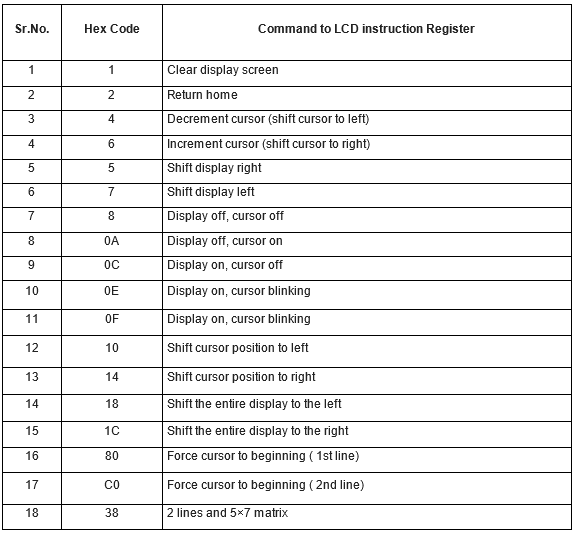
\includegraphics[width=]{f3.png}
			\end{subfigure}
		
		\end{figure}
			
			\chapter{Refrences}
			
			\section{Journal articles}
			\begin{enumerate}[label={[\arabic*]}]
			\item First item
			\item Second item
			\item \ldots
			\item Last item
		\end{enumerate}
			
			[1] 	C. Pyo, H. Gang, N. Kim and H. Bang, “Technology trends and prospects 
			of development of IoT (M2M),” OSIA Standards \& Technology Review, vol. 26, no. 2, (2013), pp. 8-17.\\
			
			{[2]}	Y. Ko, “Study of Policies of Major Countries on Internet of Things and Market Forecast,” International Commerce and Information Review, vol. 16, no. 5, (2014),pp. 27-47.\\
			
			{[3]}	D.  Seo,  H.  Ko  and  Y.  Noh,  “Design  and  Implementation  of  Digital  Door  Lock  by  IoT,”  KIISE Transactions on Computing Practices (KTCP), vol. 21, no. 3, (2015), pp. 215-222.\\
			
			[4]	S. Lee, J. Park, B. Woo and H. Choi, “Video Digital Doorlock System for Recognition and Transmission of Approaching Objects,” KIPS Transaction: Software and Data Engineering, vol. 3, no. 6, (2014), pp. 237-242.\\
			
			[5]	T. Kwak and S. Moon, “A Digital Doorlock with Voice Recognition,” in Proceedings of KIIT Spring Conference, vol. 2012,  no. 5, (2012), pp. 345-348.\\
			
			[6]	J. Potts and S. Sukittanon, “Exploiting Bluetooth on Android Mobile Devices for Home Security Application,” in Proceedings of IEEE Southeastcon Orlango, (2012), pp. 1-4.\\
			
			[7]	Y. Choi, Y. Park, W. Back, D. Lee and J. Byun, “Development of Home Automation System using Digital Doorlock based on Wireless Sensor Network,” in Proceedings of KIIT Summer Conference, vol. 2011, no. 5, (2011), pp. 189-193.\\
			
			[8]	O. Hoh and I. Ha, “A Digital Door Lock System for the Internet of Things with Improved Security and Usability,” Advanced Science and Technology Letters, vol. 109, (2015), pp. 33-38.\\
			
			[9]	H. Hassan, R. Bakar, and A. Mokhtar, “Face Recognition Based on Auto-Switching Magnetic Door Lock System Using”, in Proceedings of 2012 International Conference on System Engineering and Technology, (2012), pp.1-6.\\
			
			[10] R. Satti, S. Ejaz, and M. Arshad, “A Smart Visitors’ Notification System with Automatic Secure Door Lock using Mobile Communication Technology,” International Journal of Computer and Communication System Engineering, vol. 2, (2015), pp. 39-44.\\
			
			[11] Y. Park, P. Sthapit, and J. Pyun, “Smart Digital Door Lock for the Home Automation”, in Proceedings of TENCON 2009, (2009), pp. 1-5.\\
			
			[12]	G. Verma and P. Tripathi, “A Digital Security System with Door Lock System Using RFID Technology”, International Journal of Computer Applications, vol. 5, no. 11, (2012), pp. 6-8.\\
			
			[13]	M. Roy, F. Hemmert, and R. Wettach, “Living Interfaces: The Intimate Door Lock,” in Proceedings of the Third International Conference on Tangible and Embedded Interaction (TEI'09), (2009), pp. 45-46.\\
			
			[14]	M. Khiyal, A. Khan and E. Shehzadi, “SMS Based Wireless Home Appliance Control System (HACS) for Automating Appliances and Security”, Issues in Informing Science and Information Technology, vol. 6, (2009), pp. 887-894.\\
			
			[15]	U. Ogri, D. Okwong, and A. Etim, “Design and Construction of Door Locking Security System using GSMY”, International Journal Of Engineering And Computer Science, vol. 2,no. 7, (2013), pp. 2235-2257.\\
			
			
			
			
			\section{Conference paper}
			
			
			[16]	Yanbo Zhao ,  Zhaohui Ye "A low cost GSM/GPRS based wireless home security system" IEEE Transactions on Consumer Electronics ( Volume: 54, Issue: 2 ),2008.\\
			
			{[17]}	A. Jain , Lin Hong , R. Bolle "On-line fingerprint verification" IEEE Transactions on Pattern Analysis and Machine Intelligence ( Volume: 19, Issue: 4),1997.\\
			
			{[18]}	M. Faundez-Zanuy "A door-opening system using a low-cost fingerprint scanner and a PC" IEEE Aerospace and Electronic Systems Magazine ( Volume: 19, Issue: 8),2004.\\
			
			{[19]}	Wu Ping ;  Wu Guichu ;  Xie Wenbin ;  Lu Jianguo ;  Li Peng "Remote Monitoring Intelligent System Based on Fingerprint Door Lock" IEEE Intelligent Computation Technology and Automation (ICICTA),2010.\\
			
			{[20]}	J. Segen "A camera-based system for tracking people in real time", IEEE,1996.\\
			
			{[21]}	Jennifer L. Randall "Security system with maskable motion detection and camera with an adjustable field of view" Grant, US6727938 B1,1997.\\
			
			{[22]}	Jayashri Bangali and Arvind Shaligram "Design and Implementation of Security Systems for Smart Home based on GSM technology",International Journal of Smart Home,2013\\
			\section{[G] URL'S}
			{[17]} http://ieeexplore.ieee.org/abstract/document/587996/\\
			{[18]} http://ieeexplore.ieee.org/abstract/document/1346894/\\
			{[19]} http://ieeexplore.ieee.org/abstract/document/5522970/\\
			{[20]} http://ieeexplore.ieee.org/abstract/document/546795/\\
			{[21]} Available at https://en.wikipedia.org/wiki/GSM\\
			{[22]} Available at https://learn.adafruit.com/pir-passive-infrared-proximity-motion-sensor?view=all\\
			{[23] Datasheet of 16 X 2 available at https://electronicsforu.com/resources/learn-electronics/16x2-    lcd-pinout-diagram\\
				{[24]}https://en.wikipedia.org/wiki/Webcam\\
				{[25]}https://en.wikipedia.org/wiki/ESP8266\\
				{[26]}https://www.blynk.cc/\\
				
				
				\newpage
				
				
				
			\end{document}
			
\documentclass[twoside,a4paper,16pt]{book}
% for graphics

\usepackage[pdftex]{color,graphicx}
\usepackage[utf8]{inputenc}
\usepackage{fancyhdr}
\usepackage{amssymb}
\usepackage{parskip}
\usepackage{color}

\usepackage[textwidth=7.1in]{geometry}
\pagestyle{fancy}
\fancyhf{}
\fancyhead[LO]{\leftmark} 
\fancyhead[RE]{\rightmark}
\fancyfoot[C]{\thepage}




\let\cleardoublepage\clearpage



%set paper size
%for A4 paper
\topmargin 20mm    
%bottom margin 30mm
\oddsidemargin 20mm    
%left & right margin 15mm

%text sizes
\textwidth  180mm
\textheight 238mm
\parindent  0.00mm

%misc parameters
\headsep 3mm  
\headheight 8mm
\footskip 18mm

%\footheight 6mm

%conversion to values for LaTeX
\advance\topmargin-1.2in\advance\oddsidemargin-1.2in
\evensidemargin\oddsidemargin

%\setlength{\parindent}{3mm}



\begin{document}
	
	%%%%%%%%%%%%%%  Your Front matter Starts From here  %%%%%%%%%%%%%%%
	
	
	\frontmatter
	\thispagestyle{empty}
	
	
	%%%%%%%    Front Page  %%%%%%%%%%%%%%%%%%
	
	
	\begin{center}
		{\Large A \\ Project Stage-1 Report\\ on \\
			\vspace{0.5cm}
			
			{\bf ``Smart Security System"}}
	\end{center}
	
	\vspace{0.3cm}
	\begin{center}
		\Large Submitted in partial fulfillment for \\\vspace{0.5cm} the award of degree of\\\vspace{0.5cm}
		{\bf  BACHELOR OF TECHNOLOGY\\\vspace{0.5cm}in\\\vspace{0.5cm}Electronics \& Communication Engineering}
	\end{center}
	\vspace{0.6cm}
	
	\begin{figure}[ht!]
		\begin{center}
			
\includegraphics[width=3.0cm]{logo.jpg}
		\end{center}
	\end{figure}
	
	\vspace{0.2cm}
	
	\begin{center}
		\large Session 20{\bf17} - {\bf18}\\\vspace{0.5cm}
		{\bf Submitted by (Q.G. : 11)}\\
		{\large	\hspace{-0.1cm}Ashish Sahu (14EMBEC300)\\\hspace{0.8cm}
			Dharmendra Saini (14EMBEC016)\\\hspace{0.2cm}Santosh Yadav(14EMBEC042)\\\hspace{0.9cm}Shubham Sharma (14EMBEC051)\\\hspace{0.1cm}Vishal Yadav (14EMBEC061)}
	\end{center}
	
	\vspace{0cm}
	
	
	\Large {\underline{\bf Under The Guidance of:}} \hspace{7.5cm} {\underline{\bf Submitted To:}}\\\\
	\\
	\\
	\\
	\hspace{-1.5cm}Mrs.Hareeta Malani  \hspace{9.4cm} Mrs. Hareeta Malani  \\{\small({\bf Asst. Professor})}\hspace{11cm} {\small({\bf Project Incharge})\\
		
		
		
		
		\begin{center}
			{
				{\rule{190mm}{0.2mm}}
				\small Department of Electronics \& Communection Engineering\\
				M.L.V. Textile and Engineering College,\\(Affiliated to Rajasthan Technical University, Kota)
				\\Bhilwara 311001, Rajasthan
				\vspace{0}
				
				{\small May,2018}
			}
			
		\end{center}
		
		\newpage
		%\frontmatters
		\begin{center}
			\huge{\bf Candidate’s Declaration}\\
			
		\end{center}
		\addcontentsline{toc}{chapter}{Candidate’s Declaration}% Add title to ToC	
		{\large 
			\vspace{1.5cm}
			I hereby declare that the work presented in this project titled {“\bf Smart Security System”} submitted towards completion of project in Eighth Semester of B.Tech (ECE) at the MLV Govt. Textile and Engineering College, Bhilwara.  It is an authentic record of our original work pursued under the guidance of {\bf Mrs. Hareeta Malani (Asst. Professor)}, MLVTEC, Bhilwara. \\
			We have not submitted the matter embodied in this project for the award of any other degree. \\\vspace{.5cm}\\
			
			Ashish Sahu\\
			Dharmendra Saini\\
			Santosh Yadav\\
			Shubham Saini\\
			Vishal Yadav\\\vspace{2cm}
			
			{\bf Place: Bhilwara }\\\\
			{\bf Date: {\rule{20mm}{0.2mm}} } 
		}
		\newpage
		\noindent% just to prevent indentation narrowing the line width for this line
		\\
		\\
		
\includegraphics[width=0.10\textwidth]{logo.jpg}%
		\begin{minipage}[b]{0.8\textwidth}
			\centering
			{\large {\bf M.L.V. Govt. Textile \& Engineering College, Bhilwara} }\\
			(An Autonomous Engineering College of Govt. of Rajasthan)\\
			Department of Electronics \& Communication
		\end{minipage}%
		
\includegraphics[width=0.11\textwidth]{rtu.png}\\
		\\
		
		\begin{center}
			\huge{\bf Bonafide Certificate} 
		\end{center}
		\addcontentsline{toc}{chapter}{Bonafide Certificate}
		\vspace{2cm}
		{\large This is to certify that the project work entitled {\bf “Smart Security System”} is carried out by\\
			\vspace{.5cm}\\
			Ashish Sahu \\
			Dharmendra Saini\\
			Santosh Yadav\\
			Shubham Sharma\\
			Vishal Yadav\\
			\\
			Under my supervision and guidance during the academic year 2017-18 and to the best of our knowledge is original work.\\
			\\
			Submitted for viva-voce examination held on Date :\\
			\vspace{2cm}\\
			Project Guide\hspace{3.5cm}Internal Examiner\hspace{3.5cm}External Examiner\\
			\vspace{1cm}\\
			(Mrs. Hareeta Malani)\hspace{1.8cm}(Mrs. Hareeta Malani)\hspace{2.8cm}(Name of external examiner)
			\newpage
			\begin{center}
				\huge{\bf Acknowledgement} 
			\end{center}
			\addcontentsline{toc}{chapter}{Acknowledgement}
			\vspace{1.5cm}
			
			{\large We take immense pleasure in thanking {\bf Dr. A. K. Chaturvedi, Principal} MLVTEC for permitting us to carry out this project work.\\
				We give our thanks to HOD {\bf (Mr. Ritesh Saraswat)}, Project In-charge{\bf (Mrs. Hareeta Malani)} and to my college MLVTEC for their extreme co-operation.\\
				We pay our thanks to {\bf Mrs. Hareeta Malani (Asst. Professor)} and {\bf Mrs. Priyanka Kabra} for their encouragement and appreciations we have received.\\
				We are also thankful to all the faculty members, for the valuable suggestions and the guidance.\\
				Finally, yet importantly, we would like to express our heartfelt thanks to our beloved parents for their blessings, my friends/classmates for their help and wishes for the successful completion of this project.\\
				
				
				\vspace{2cm}
				Ashish Sahu\\
				Dharmendra Saini\\
				Santosh Yadav\\
				Shubham Saini\\
				Vishal Yadav\\ \\}
			\newpage
			\begin{center}
				\huge{\bf Abstract}
			\end{center}
			\vspace{1.5cm}
			\addcontentsline{toc}{chapter}{Abstract}
			\large Home security has been a major issue where crime is increasing and everybody wants to take proper measures to
			prevent intrusion. In addition there was a need to automate home so that user can take advantage of the technological
			advancement in such a way that a person getting off the office does not get melted with the hot climate. Smart
			security system is project in which we provide users to use such type of technology and improve security of home and
			office. By using such type of technology we can control unwanted activity. Purpose behind developing this project is
			that to protect from theft to our society and also protect from criminal. In this we will develop a security system in
			which authorized users can enter in home or office every member of home or office will be identified by its finger print
			or face by using biometric and all these details will be stored on a web page which can be access by admin only and
			in case of unauthorized person an image of that person will be send on server as well as on mobile phone of admin.
			This advance security system also has feature that door of the office or home will not be unlocked until user is not
			authorized. All activity like who entered in home will be store and also notify on mobile phone to a particular no.
			such type of technology is very useful for those industries in which they required privacy and it can be used also at
			home and these all activities through a remote or a mobile. For developing such type of project we required some
			concept of IOT and MATLAB for image processing of fingerprint.\\\\
			Keywords : Security Systems, Finger Print Access, CCTV Security, Embedded Systems, Internet Of Things, Image
			Processing, MATLAB\\
			
			
			\newpage
			\mainmatter
			\tableofcontents
			\listoffigures
			\listoftables
			
			
			\contentstyleisdeshed
			
			\newpage
			\chapter{Smart Security System}
			\section{Introduction}
			The Internet of Things (IoT) can be defined as a global infrastructure which combines
			intelligent services with situational awareness, and allows mutual communication
			between one thing and another, and between people and intelligent things over a network
			[1]. Machine to Machine (M2M) communication is different from IoT because a person
			does not directly control the equipment or intelligent instruments; they are responsible for
			communicating on behalf of people [2].
			More recently, a variety of communication technologies have been fused to receive and
			provide information about things. Especially, IoT technologies have been enabled to
			communicate by the fusion of home appliances and mobile devices.
			Recently, digital door locks have been widely used in households and offices.
			However, in many cases, an intruder has tried to penetrate a private area by circumventing
			the lock. In this study, we design and implement an IoT-based digital door lock to reduce
			the damage of digital door lock tampering and to enhance the various security and
			monitoring functions using IoT technologies.
			
			\begin{figure}[ht!]
				\begin{center}
					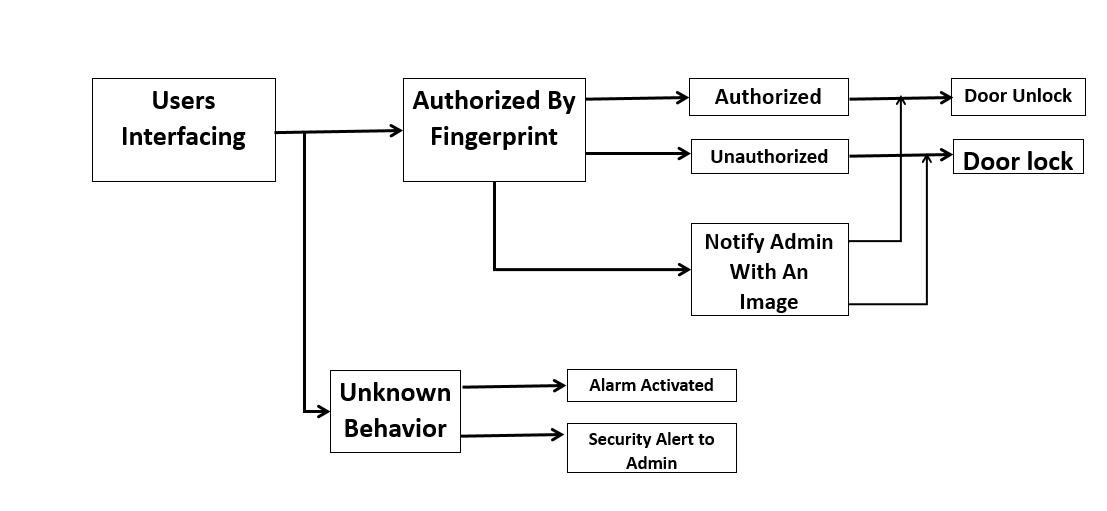
\includegraphics[width=10.0cm]{b1.jpg}
					\caption{Basic Overview}
				\end{center}
			\end{figure}
			When a message was received from the GSM then the micro controller will display that message on LCD at the end
			of the message a number is received based on that number the micro controller will does the coresponinding operation
			to that number like switching the devices ON and OFF. and the date and time of that message received is displayed
			on LCD display.
			\section{Background}
			\section*{Security in the Early Days}
			The home alarm system as we know it today wasn't present during the Stone Age. Cavemen used other means of protection to keep predators at bay. Initially, they used branches and rocks, and later on they created slingshots, and bows and arrows. As time progressed, domesticated wolves were used to protect homes. People would rescue abandoned wolf cubs and raise them to protect their possessions. Eventually, this lead to the guard dogs we know today. In ancient Egypt, around 3150 BC, people would dig trenches around their dwellings, towns, and fortresses. These trenches, also known as moats, were filled with water and used to protect the people from intruders. With the growth of businesses and business ownership during the mid-1700s, people started using security guards to protect their properties. The royals also used security guards for their personal protection. Today, the human touch is still used to offer protection.
			\section*{Home Security Systems Today}
			Today's home security systems are either linked to a landline, or cellular or broadband connection. When the alarm is set off, any one of these three systems can communicate with the monitoring center. If you don't turn off the alarm within a certain period, the center will call you to inquire about the alarm. If it's a false alarm, you must provide your password to stop all further action. If no password is given, or if you don't respond to the call, the police will be sent over to your resident to ensure that there's no burglary taking place. Some home alarm systems can be controlled through your cell phone or tablet. In addition to arming and disarming the alarm system, mobile access to your alarm system can come with other features. You can, for instance, unlock and lock doors, turn the lights on or off, set the thermostat, and more. You can also install a security system with cameras that record every action that occurs on your property. This type of security is often used by business owners. Also, if you're renting a home, or if you plan on moving in a few years, you can install a wireless alarm. This allows you to take your alarm system with you when you move. Some other features that are available when it comes to home security include a glass break sensor, smoke detectors, flood sensors, and carbon monoxide and motion detectors.\\
			
			\section{Aim of this Project}
			The aim of our project is to provide privacy and security to a particular Home or companies from remote loca-
			tions from a central Server system. The idea of having a full control over the places where we live and work has always
			been a fascinating subject to fantasize no matter at what age! As the technology improved in recent decades, human
			being gained more power on controlling various devices indoors. However, having this control remotely still remains
			an incomplete yet developing matter in industry.
			The Project entitled SMART SECURITY SYSTEMS highlights the above mentioned issue and oers ways to
			overcome this need by employing two of the most widely used features of todays technology SMS to be applied as a
			bridge in between human and fully automated buildings, GSM standard which ensures perfect compatibility between
			networks and mobile phones in any location.
			In this project, the system allows the home owner or company owner to monitor and control the house security like
			Whose entered, Door lock or door unlocked, which can be switched on or o via the mobile phone set by sending
			commands in the form of SMS and also the home owner can receive the appliances status.
			\section{History}
			According to the Bureau of Justice Statistics, household burglaries in the United States have declined by 56 percent from 1994 to 2011. It's believed that residential security systems are partly responsible for this decline. Burglars are less likely to break into a home that's secured with an alarm system. If a secured house is invaded, an audible alarm system will often scare off the criminals and stop them in their tracks. Technological developments have made today's home alarm systems ultra-modern, high-tech gadgets. To understand how these developments came about, it's worth exploring the history of home security.\\
			
			\section{ Methodology}
			
			The overall structure of the proposed system is shown in Figure 1.2. The proposed system consists of a digital door lock, two Atmega 8 control board that is mounted in the lock, and the end-user’s mobile device.
			The controller detects physical impacts applied by a visitor, and notifies the user’s mobile device. The controller detects if a invalid fingerprint error occurs more than a certain number of times, and uses the camera to capture an image of the visitor. It then transfers the image to the user’s mobile device. All of the access records are stored in the controller’s database, which can be queried via the user’s mobile device.
			\begin{figure}[ht!]
				\begin{center}
					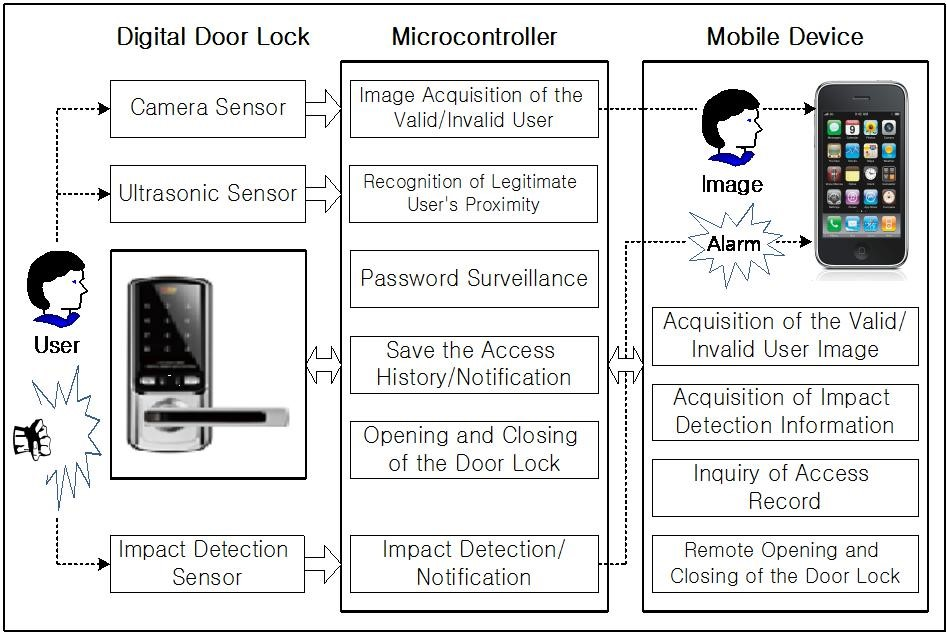
\includegraphics[width=13.0cm]{f1.jpg}
					\caption{Methodology [16]}
				\end{center}
			\end{figure}
			If a visitor has lost his key, his image is captured and transferred to the user’s mobile device by pressing a specific key; the user can then control the door lock remotely after verifying whether the visitor is valid. Another important function of the controller is automatically opening or closing the door when a valid user comes near. When a valid user accesses the gate holding an object, because it is difficult to operate the door lock, the controller communicates with the user’s mobile device via wireless and opens the door lock automatically.
			
			The mobile device acquires the impact detection information and the invalid visitor image information from the controller, and then the user can take appropriate action. Further, if the user acquires image information for a valid visitor, it is possible to open or close the door lock remotely. It is also possible to query the incoming and outgoing
			
			\section{Significance of this Work}
			The main features of the proposed system are as follows. First, it has impact detection
			and alarm functions. This is to detect an intruder who tries to invade by applying physical
			force to the lock. Second, it has an image transfer function. Generally, an attacker who.does not know the password will make a variety of attempts. Therefore, if an attacker
			mistypes the password or fingerprint is not recognized more than a given number of times, the system obtains images of
			the intruder and transfers them to the mobile device.
			Third, the user can query the records of detected face and all incoming and
			outgoing records that are stored in the database. Fourth, the system can open the door lock
			in real-time after recognizing a visitor’s image. If a visitor forgets the password, he can
			type a code into the door lock; then, the door lock system transmits his image to the
			mobile device user. The user can remotely control the door lock after reviewing the
			image. Fifth, the controller can detect a valid user approaching the digital door lock, if he
			is carrying the mobile device, and will open or close the door lock automatically.
			
			\section{Outline}
			The controller detects physical impacts applied by a visitor, and notifies the user’s
			mobile device. The controller detects if a password error occurs more than a certain
			number of times, and uses the camera to capture an image of the visitor. It then transfers
			the image to the user’s mobile device. All of the access records are stored in the
			controller’s database, which can be queried via the user’s mobile device.
			If a visitor has lost his key, his image is captured and transferred to the user’s mobile
			device by pressing a specific key; the user can then control the door lock remotely after
			verifying whether the visitor is valid. Another important function of the controller is
			automatically opening or closing the door when a valid user comes near. When a valid
			user accesses the gate holding an object, because it is difficult to operate the door lock,
			the controller communicates with the user’s mobile device via Bluetooth and opens the
			door lock automatically.
			The mobile device acquires the impact detection information and the invalid visitor
			image information from the controller, and then the user can take appropriate action.
			Further, if the user acquires image information for a valid visitor, it is possible to open or
			close the door lock remotely. It is also possible to query the incoming and outgoing 
			\section{Conclusion}
			The GSM and IOT based advance security system has been designed and tested with the mobile
			network. The user can get alerts anywhere through the GSM technology thus making the
			system location independent. A flexible way to control and explore the services of the mobile,
			AT commands is used in the system. The communication of home is only through the SMS
			which has been tested with the mobile networks and is working on any mobile network.
			The web camera based security system is very easy, user friendly and software has many
			features. It will be more easy to use IP camera instead of web camera. However, the cost of IP
			camera is more. Similar softwares are available on internet which will perform the same task.
			This type of system is useful when the owner is out of station and the home is locked. By
			installing the web camera at the door site, intruder can be detected and owner can receive a \\
			mail telling the intruder entry in a home. If the nearby police station email id is also
			configured in the system, then the intrusion mail can be received by police also and necessary
			action can be taken.
			The system has tested on the model of smart home and further it will be tested in actual
			home. The complexity of the algorithm of the system can be increased by introducing number
			of sensors to make the energy efficient home. 
			\chapter{Literature Review }
			Seo et al. [3] studied convenient digital door lock functions, such as remote control via the integration of mobile devices and key sharing. Lee et al. [4] proposed a method for detecting an accessing object and transmitting the object image. Kwak et al. [5] studied a method for opening and closing the door lock using voice recognition, without using a network. Potts et al. [6] proposed a security system that interfaces with an Android mobile device. The mobile and security system communicate via Bluetooth in a short range. Choi et al. [7] developed an application for communication between devices for transferring the state of the alarms generated in a home through a door lock in the neighborhood.
			
			Hassan et al. [9] and Satti et al. [10] studied face recognition for the door lock open. In particular, the application of Satti et al. transfers the SMS about the legitimacy of the user to the mobile device. However, both of them cannot be a perfect IoT application because the door locks are not controlled by the mobile device remotely. Studies of Park et al. [11] and Verma et al. [12] are related to security applications for home automation. Studies of Khiyal et al. [14] and Ogri et al. [15], are initial studies [13] for remotely controlling a door lock, which cannot be classified also into application of the complete IoT.
			
			The system proposed in this study strengthens the security functions. For example, if a physical impact is added to the intrusion attempt, the system notifies the user of the intrusion through the user’s mobile device. Further, if someone inputs erroneous pass-codes more than a certain number of times, the system captures and transmits an image of the person [8].
			
			To reduce the burden on the network, the proposed system transmits an image only when the input pass-code fails, unlike [4], which transmits a video of all accessing objects. In addition, it provides basic functions, such as remote control access and viewing all incoming and outgoing information that has been recorded on the system.
			
			\section{Existing  technologies related to our project}
			The proposed system provides strengthened security functions that can transfer recorded images to a user’s mobile device when an invalid user attempts an illegal operation; it can also deliver alarm information to the mobile device when the door lock is physically damaged. The proposed system enables a user to check the access information and remotely operate the door lock to enhance convenience.\\
			
			\newpage
			
			\begin{center}
				\begin{table}[h!]
					\centering
					\begin{tabular}{|p{2cm}|p{6cm}|p{5cm}|}
						\hline
						Study (Year) & Main Function & Networking\\
						\hline	
						(2015) & [3]Connecting to mobile devices,Key sharing,mobile device,Access notification & Connection to a mobile device,via Bluetooth\\
						\hline
						(2014) & [4] Image transfer & Connection of mobile devices\\
						\hline
						(2012) & [5] Door opening and closing by speech recognition & –	\\
						\hline
						(2012) & [6] Controlling door lock in a short range with a mobile application & Communication via Bluetooth\\
						\hline
						(2011) & [7] Diffusion of alarm using the door lock & Interconnection of door locks\\
						\hline
						(2012) & [9] Face Recognition & –\\
						\hline
						(2015) & [10] Face Recognition and automatic open & Sending SMS to Mobile phone\\
						\hline
						(2015) & [11] Door Lock for the home automation & –\\
						\hline
						(2010) & [12] Security application for door lock & –\\
						\hline
						(2009) & [14] Basic applications for remote control & Remote control\\
						\hline
						(2013) & [15] Impact detection / notification,Image transfer,Recording access information,Image recognition / remote control,Recognition of user proximity and automatic open & Connection to a	mobile device\\
						\hline	
					\end{tabular}
					\caption{Existing  technologies related to our project}	
				\end{table}
			\end{center}
			The prevention of unauthorized entry into buildings
			through the main doors is done by using ordinary,
			electronically operated locks, digital codes and biometrics
			technique like the finger print technology or some are
			based on thumb printing only. Nowadays, advanced
			automatic door security systems are available with the use
			of palmtop recognition systems face recognition systems,
			face detection systems, wireless sensors, PIR sensors,
			RFID techniques, smart cameras and many more that helps
			people to make their home or organizations secure from
			long distance. Hence, people need not to be worry about
			the home security though they are away from home.
			\section{Introduction  (Study of papers)}
			Recently, digital door locks have been widely used as part of the IoT (Internet of Things). However, the media has reported digital door locks being opened by invalid users to invade homes and offices. In this study, a digital door lock system that can work with the IoT environment is proposed. It is designed and implemented to enhance security and convenience.
			
			The proposed system provides strengthened security functions that can transfer recorded images to a user’s mobile device when an invalid user attempts an illegal operation; it can also deliver alarm information to the mobile device when the door lock is physically damaged. The proposed system enables a user to check the access information and remotely operate the door lock to enhance convenience.
			Security represents protection of our life and assets.
			Ensuring safety of peoples and their valuable things is very
			important for the prevention of illegal handling. Hence,
			mainly focusing on door lock security or gate security is
			very important to avoid the further problems in monitored
			area. Even with the use of mechanical locks, the crime,
			robberies get happened due to the fact that such locks were
			easily broken. So, there is a need to invent other kind of
			locks which cannot be easily broken. So, many authors
			present different kinds of digital door locks, automatic
			password based door locks, software based door locks etc.
			which have been widely used in houses and offices.
			\\
			In latest password based system, a more advanced system
			develops which communicates the owner of the office
			or house, when any unauthorized person tries to open the
			code, by giving correct code as well. While closing the
			door of office/home, the owner has to press the „0‟ key
			available on the hex keypad and leave the system. The
			system developed by Annie P. Oommen et. al.  allows
			for changing the password. To open the lock, the entered
			password must matches with the changed one. In some
			systems the security dial-up enables through the GSM
			modem , when the unauthorized person enters an invalid
			password then the controller informs to the owner through
			GSM modem. Latest security system  is designed where
			the locking security system can be enhanced with the help
			of RF and GSM wireless technology by using a 4 digit
			password which provides the authentication.
			Keywords: Door Lock Security, GSM, RFID, SMS, Sensors, Camera,
			Alarm, Biometrics, WI FI, Password, Internet of things
			\section{Research Approach}
			Redefining 'security' has recently become something of a cottage industry. 1 Most
			such efforts, however, are more concerned with redefining the policy agendas of
			nation-states than with the concept of security itself. Often, this takes the form of
			proposals for giving high priority to such issues as human rights, economics, the
			environment, drug traffic, epidemics, crime, or social injustice, in addition to the
			traditional concern with security from external military threats. Such proposals are
			usually buttressed with a mixture of normative arguments about which values of
			which people or groups of people should be protected, and empirical arguments as
			to the nature and magnitude of threats to those values. Relatively little attention is
			devoted to conceptual issues as such. This article seeks to disentangle the concept of
			security from these normative and empirical concerns, however legitimate they
			may be.
			Cloaking normative and empirical debate in conceptual rhetoric exaggerates the
			conceptual differences between proponents of various security policies and impedes
			scholarly communication. Are proponents of economic or environmental security
			using a concept of security that is fundamentally different from that used by
			Realists? Or are they simply emphasizing different aspects of a shared concept? Do
			those who object to 'privileging' the nation-state rather than, say, the individual or
			humanity share any conceptual views with students of 'national security'? \\
			\\
			it is important to be clear about the limits of this approach. Explicating the
			concept of security does not provide empirical propositions, theories, or analytical
			frameworks. Although clear concepts are useful for constructing propositions.
			theories, and analytical frameworks, they are not a substitute for them. 
			\begin{center}
				\begin{table}[h!]
					\centering
					\begin{tabular}{|p{.8cm}|p{3cm}|p{3cm}|p{3cm}|p{4.5cm}|p{1cm}|}
						\hline
						S.NO. & Artical & Authpr & Publication & CONCLUSION &YEAR \\ \hline
						
						1. & Security and Usability Improvement on a Digital Door Lock System based on Internet of Things & Ilkyu Ha &	Researchgate (December 2016) & In this paper we get an algorithm for implementation of digital door lock & 2015 \\
						\hline
						2. & Technology trends and prospects of development of IoT (M2M) & C. Pyo, H. Gang, N. Kim and H. Bang & OSIA Standards Technology Review, vol. 26, no. 2, & This article was helpful for understanding the concept of internet of things & 2013\\
						\hline
						3. & A low cost GSM/GPRS based wireless home security system & Yanbo Zhao ,  Zhaohui Ye	& IEEE Transactions on Consumer Electronics ( Volume: 54, Issue: 2 ) & In this paper we found that how we can implement a low cost wireless security system & 2008\\
						\hline
						4. & On-line fingerprint verification & A. Jain , Lin Hong , R. Bolle & IEEE Transactions on Pattern Analysis and Machine Intelligence ( Volume: 19, Issue: 4) & This paper was helpful in understanding the concept of fingerprint verification & 1997\\
						\hline
						5. & A door-opening system using a low-cost fingerprint scanner and a PC &	M. Faundez-Zanuy & IEEE Aerospace and Electronic Systems Magazine ( Volume: 19, Issue: 8) & This paper helped us to develop a low cost fingerprint access door lock systems & 2004\\
						\hline
						6. & Remote Monitoring Intelligent System Based on Fingerprint Door Lock & Wu Ping ;  Wu Guichu ;  Xie Wenbin ;  Lu Jianguo ;  Li Peng & IEEE Intelligent Computation Technology and Automation (ICICTA) & In this paper we get algorithms for monitoring of security system based on fingerprint & 2010\\
						\hline
						7. & A camera-based system for tracking people in real time & J. Segen & IEEE & This paper was helpful for development of camera on a system which can monitor real time tracking & 1996\\
						\hline
						8. & Security system with maskable motion detection and camera with an adjustable field of view & Jennifer L. Randall & Grant, US6727938 B1 & In this paper we found algorithm for implement a motion detection system & 1997\\
						\hline
						9. & Design and Implementation of Security Systems for Smart Home based on GSM technology & Jayashri Bangali and Arvind Shaligram & International Journal of Smart Home & This papers helped us to know interfacing of GSM technology with security system & 2013\\
						
						
						
						\hline
						
					\end{tabular}
					\caption{Research Approch}	
				\end{table}
				
			\end{center}
			\newpage
			\section{Modules of project }
			The design of a biometric and web cam based door locking security system using IOT and MATLAB is a complex design which
			comprises of so many modules (parts) brought together to form the overall design. Each of these modules is
			made up of discrete components and modules that are joined together to achieve a particular purpose. 
			These separate modules are: The Power Supply Unit, The Buzzer Unit, The micro controller Unit, Webcam unit, Biometric unit, GSM unit, Image processing unit
			Switching unit.
			These different units can be function alone, for the desired result they all need to function together. We have divided our proposed system into four Module which is as follow.
			\subsection{Survey}
			The researchers gathered information from different sources which give appropriate ideasor what parts to be used in every circuitry involved in this project. Keypad interfacing tomicrocontroller using embedded C was the hardest part ever encountered during thedevelopment stage. From a step by step process, researchers started from writing simplecode to more complex. After everything is fixed and tested in virtual simulation, the researchers soldered everything for implementation stage. Researchers faced many problems on hardware such as fine tuning every sensor to work simultaneously with the burnt program inside the microcontroller. By eliminating those problems gives good andaccurate anticipated result. Same project could have been designed with 8051 microcontroller,Arduino
			\subsection{Study of Software and Hardware}
			\begin{enumerate}
				\item Study of required software (ATmel studio, Proteus Design Suit, Microchip, MATLAB, IOT, )
				\item Study of required hardware and component (Atmega 8, RS305 Fingerprint sensor, GSM Module, Motion Sensor, ESP 8266 wifi Module, LCD)
			\end{enumerate}
			\subsection{Design of the Advance Security System}
			\begin{enumerate}
				
				\item Overall Structure of the Proposed System
				\item Main Features of the Proposed System
			\end{enumerate}
			\subsection{Implementation}
			\begin{enumerate}
				
				\item Hardware Components and Configuration of the Proposed System
				\item Apps for Remote Control
				\item Testing
			\end{enumerate}
			\newpage
			\chapter{System Architecture}
			\section{Overview}
			There are two parts in our project. They are the
			security system and the load controlling system. In the
			security system we use several sensors such as
			Biometric sensor, Webcam, motion sensor. In
			the load controlling system we use relay to on or off the
			load. We have used GSM module to send message to a
			subscriber identification number about security purpose. We have also used this GSM module to control load from remote area. The whole project have been designed in the Proteus software. Each part of our project has been discussed in
			details 
			\subsection{Load controlling system}
			Protection of home main door is the important part in
			security system which done in this system by using
			electromagnetic lock in conjunction with fingerprint module. The
			owner using this biometric for valid user which is display
			on LCD and if the fingerprint matched is correct then the
			electromagnetic lock is opened. Otherwise if does not matched, the door will still locked.\\
			In this project the main and second priority unit is load
			control which has been interfaced with microcontroller.
			Load can be turned on or off by sending message from
			mobile phone. In our project we have controlled two
			loads via microcontroller and GSM module. We can
			also receive update of which load is on or which load is
			off if we want to know it.
			\subsection{Motion detector or Theft Detection unit} 
			The motion sensor gives digital output which has been
			used as microcontrollers input. When motion has been
			detected, motion detector gives logical one to the
			microcontroller. Then microcontroller takes necessary
			decision by reading the detector output. As a motion
			sensor we used PIR sensor which allow you to sense
			motion, almost always used to detect whether a human
			has moved in or out of the sensor's range. They are often
			referred to as PIR, "Passive Infrared", "Piezoelectric", or
			"IR motion" sensors. PIRs are basically made of a
			piezoelectric sensor (which you can see above as the
			round metal can with a rectangular crystal in the centre),
			which can detect levels of infrared radiation. The PIR
			sensor itself has two slots in it; each slot is made of a
			special material that is sensitive to IR. The lens used here
			is not really doing much and so we see that the two slots
			can 'see' out past some distance (basically the sensitivity
			of the sensor).\\
			In theft detection system, simple mechanism has been used.
			When a object has been passed through the door wile sensors are on, buzzers and AC bulbs are connected with 220 volt through the relay and detected as per the microcontroller input port. Then microcontroller takes necessary decision by
			reading the input port. When a object has been passed, logic
			high input to the microcontroller pin.
			\begin{figure}[ht!]
				\begin{center}
					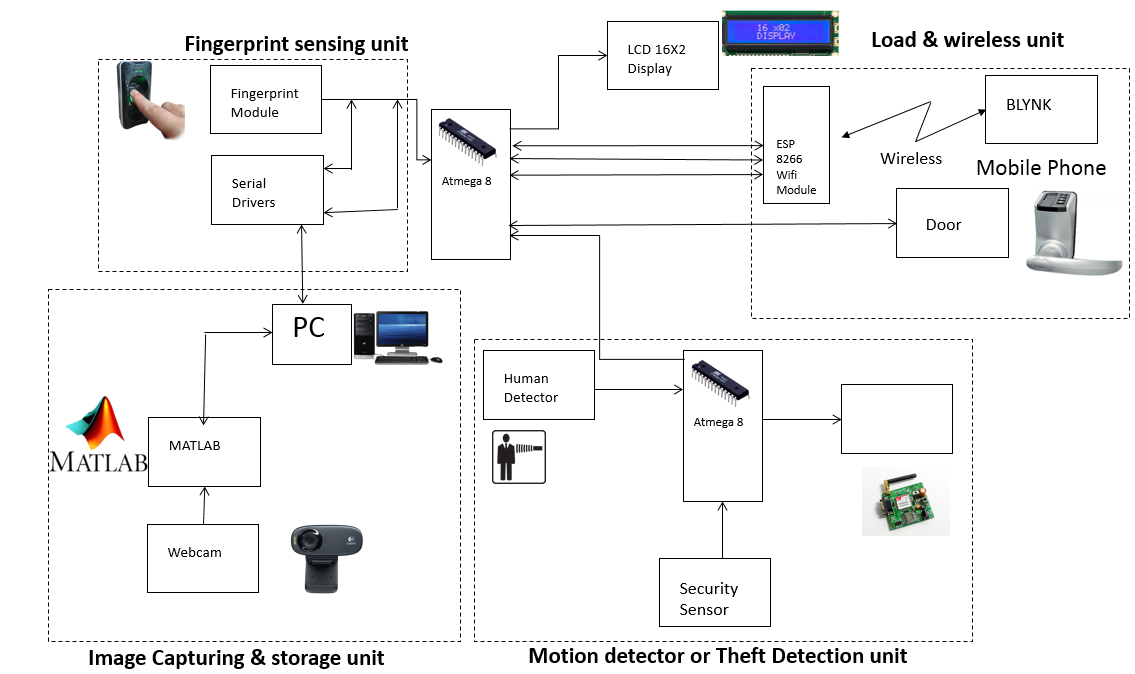
\includegraphics[width=17.0cm]{b2.png}
					\caption{Main Block Diagram}
				\end{center}
			\end{figure}
			\subsection{Fingerprint sensing unit}
			This unit monitors real time fingerprint verification data from 
			doors. This unit has its setting  limitted tryels. Above this  value, the microcontroller sends message to the user‟s mobile phone that the
			someone tryed to acces door and crossed its limitted tryel.
			In case if user is verified than an output will send through the microcontroller to the load for unlock the door. We have used RS305 as fingerprint sensor.
			
			\subsection{Image Capturing \& storage unit}
			By default the first camera is selected, but we can select any of the available devices from the
			listbox .After the device is selected, the camera is interfaced through coding part. Then there is a button
			‘Activate Motion Detection’, through which we can select the mode of our working and the application is set on Whenever any unvalid user tryed to access then application
			starts capturing the images and they are stored into a folder using. At the same time , a wireless signal is transmitted to the receiver through ESP8266 module using blink application and wait for desired action taken from the owner side.
			\section{Reaction of sensors \& Flow chart}
			\subsection{Reaction of Sensors}
			Figure 3.2 shows the reaction time of each sensor. All of the sensors act to actions of the valid and invalid user in 2 seconds. For example, the ultrasonic sensor can take from 1.6 seconds to 1.8 seconds to check a valid user and open the door. One of the most important features of our proposed system is to check an invalid password of an invalid user. It takes 1.41 seconds on average to detect an invalid password, take a picture of the user and send the picture to a mobile device.
			\begin{figure}[ht!]
				\begin{center}
					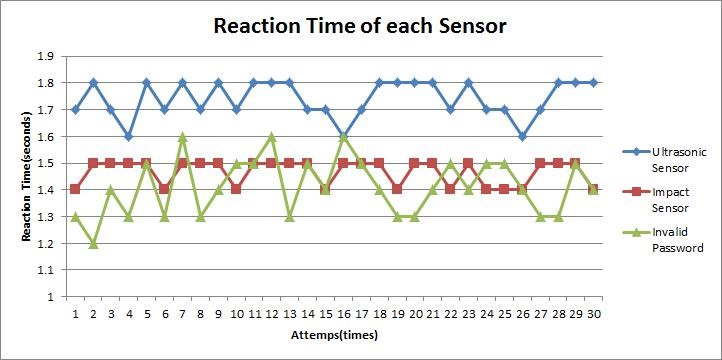
\includegraphics[width=12.0cm]{f5.jpg}
					\caption{Reaction of each sensors [16]}
				\end{center}
			\end{figure}
			The proposed digital door lock system in this study has several implementation problems. The first problem concerns the image captured by the camera's sensor when an incorrect password is entered. If the invader intentionally covers the camera lens or deviates the focus from him, it will be impossible to collect an accurate image. Second, since the shock sensor senses a certain amount of impact whenever the door opens or closes, it is difficult to distinguish an abnormal impact. These problems will be resolved as future challenges.
			\subsection{Flow Chart}
			In this flow chart two cases are discussed in which one is for valid user and another one is for invalid user all the activity of these usr will be capture and can be store and also there are limited no of tryels for each.Besides, various sensors for proximity and intrusion detection are connected to the system. A camera sensor for photographing an image of invalid users is installed, an impact sensor is attached for detecting a physical shock by an invalid user, and an ultrasonic sensor is attached to recognize the proximity of valid users.\\\\
			When an access request is generated by a valid visitor who does not possess the key, the ‘Request’ menu allows the user to check the image of the requester and open the door. The ‘Remote opening’ menu allows for remote door operation. The ‘Option’ menu allows for password management and ‘Bluetooth synchronization (Master mode)’ menu is a setting menu for automatic opening when approaching the door lock. Figure 6 shows the application cases for remote controls. The left side of the top of the figure is the main menu of the App, the right of the top shows the Bluetooth setup button for proximity open and a keypad for the remote open. The left of the bottom of the figure shows a list of the image information that has been captured by physical shock and the input mistake of password. And the right of the bottom shows an image of the item in the list.
			
			
			
			
			\begin{figure}[ht!]
				\begin{center}
					\includegraphics[width=16cm]{f6.png}
					\caption{Flow Chart of Project}
				\end{center}
			\end{figure}
			\section{Algorithm}
			STEP 1  : \hspace{0.2cm} {\bf START}\\
			STEP 2  : \hspace{0.2cm} {\bf FOR} each user\\
			STEP 3  : \hspace{0.6cm} {\bf INPUT} Action\\
			STEP 4  : \hspace{0.6cm} {\bf SWITCH} Action\\
			STEP 5  : \hspace{1cm} {\bf CASE} ``fingerprint"\\
			STEP 6  : \hspace{1.4cm} {\bf IF} fingerprint does not match {\bf THEN} take and send image\\
			STEP 7  : \hspace{1.4cm} {\bf ELSE IF} fingerprint is valid {\bf THEN} open the door\\
			STEP 8  : \hspace{1.4cm} {\bf ELSE IF} number of mismatch greater then 3 {\bf THEN} take and send image\\
			STEP 9  : \hspace{1.8cm} {\bf ELSE} go to STEP 2\\
			STEP 10 : \hspace{1cm} {\bf CASE} ``impact"\\
			STEP 11 : \hspace{1.cm} Impact Sensor operation\\
			STEP 12 : \hspace{1.4cm} {\bf IF} impact value greater then threshold valu {\bf THEN} camera sensor operation\\
			STEP 13 : \hspace{1.4cm} {\bf ELSE} go to STEP 2\\
			STEP 14 : \hspace{1cm} {\bf CASE} ``proximity"\\
			STEP 15 : \hspace{1.4cm} {\bf IF} distance greater then threshold value {\bf THEN} mobile device synchronization\\
			STEP 16 : \hspace{1.6cm} {\bf IF} valid user {\bf THEN} open the door\\
			STEP 17 : \hspace{1.6cm} {\bf ELSE} go to STEP 2\\
			STEP 18 : \hspace{1.4cm} {\bf ELSE} go to STEP 2\\
			STEP 19 : \hspace{0.2cm} {\bf END}
			
			\chapter{\bf Implementation of Project }
			\section{Software Requirement }
			\subsection{ATmel Studio}
			AVR Studio 6 is a software development environment developed by Atmel. It is meant to replace AVR Studio 5 going forward providing a single development platform for Atmel's 8-bits, 32-bits and ARM Cortex-M families of AVR microcontrollers.AVR is a family of microcontrollers developed by Atmel beginning in 1996. These are modified Harvard architecture 8-bit RISC single-chip microcontrollers. AVR was one of the first microcontroller families to use on-chip flash memory for program storage, as opposed to one-time programmable ROM, EPROM, or EEPROM used by other microcontrollers at the time.
			
			AVR microcontrollers find many applications as embedded systems; they are also used in the Arduino line of open source board designs.
			
			\begin{figure}
				\begin{center}
					\includegraphics[width=10.0cm]{cc.png}
					\caption{ATmel Studio Interface}
				\end{center}
			\end{figure}
			\subsection*{Brief History}
			
			The AVR architecture was conceived by two students at the Norwegian Institute of Technology (NTH),[1] Alf-Egil Bogen[2] and Vegard Wollan.[3]
			
			The original AVR MCU was developed at a local ASIC house in Trondheim, Norway, called Nordic VLSI at the time, now Nordic Semiconductor, where Bogen and Wollan were working as students.[citation needed] It was known as a μRISC (Micro RISC) and was available as silicon IP/building block from Nordic VLSI. When the technology was sold to Atmel from Nordic VLSI, the internal architecture was further developed by Bogen and Wollan at Atmel Norway, a subsidiary of Atmel. The designers worked closely with compiler writers at IAR Systems to ensure that the AVR instruction set provided efficient compilation of high-level languages.
			Atmel says that the name AVR is not an acronym and does not stand for anything in particular. The creators of the AVR give no definitive answer as to what the term "AVR" stands for.However, it is commonly accepted that AVR stands for Alf and Vegard's RISC processor.Note that the use of "AVR" in this article generally refers to the 8-bit RISC line of Atmel AVR Microcontrollers.
			
			Among the first of the AVR line was the AT90S8515, which in a 40-pin DIP package has the same pinout as an 8051 microcontroller, including the external multiplexed address and data bus. The polarity of the RESET line was opposite (8051's having an active-high RESET, while the AVR has an active-low RESET), but other than that the pinout was identical.
			
			The AVR 8-bit microcontroller architecture was introduced in 1997. By 2003, Atmel had shipped 500 million AVR flash microcontrollers. The Arduino platform for simple electronics projects was released in 2005 and featured ATmega8 AVR microcontrollers.
			\subsection{Proteus Design Suite}
			The Proteus Design Suite is a proprietary software tool suite used primarily for electronic design automation. The software is used mainly by electronic design engineers and technicians to create schematics and electronic prints for manufacturing printed circuit boards.
			Proteus is a simulation and design software tool developed by Labcenter Electronics for Electrical
			and Electronic circuit design. It also possess 2D CAD drawing feature. It deserves to bear the tagline ``From concept to completion”.
			It was developed in Yorkshire, England by Labcenter Electronics Ltd and is available in English, French, Spanish and Chinese languages.
			\subsection*{History}
			The first version of what is now the Proteus Design Suite was called PC-B and was written by the company chairman, John Jameson, for DOS in 1988. Schematic Capture support followed in 1990, with a port to the Windows environment shortly thereafter. Mixed mode SPICE Simulation was first integrated into Proteus in 1996 and microcontroller simulation then arrived in Proteus in 1998. Shape based autorouting was added in 2002 and 2006 saw another major product update with 3D Board Visualisation. More recently, a dedicated IDE for simulation was added in 2011 and MCAD import/export was included in 2015. Feature led product releases are typically biannual, while maintenance based service packs are released as required.
			\subsection*{Features}
			ISIS has wide range of components in its library. It has sources, signal generators, measurement  and analysis tools like oscilloscope, voltmeter, ammeter etc., probes for real time monitoring of the parameters of the circuit, switches, displays, loads like motors and lamps, discrete components like resistors, capacitors, inductors, transformers, digital and analog Integrated circuits, semi-conductor switches, relays, microcontrollers, processors, sensors etc.
			
			ARES offers PCB designing up to 14 inner layers, with surface mount and through hole packages. It is embedded with the foot prints of different category of components like ICs, transistors, headers, connectors and other discrete components. It offers Auto routing and manual routing options to the PCB Designer. The schematic drawn in the ISIS can be directly transferred ARES.
			\begin{itemize}
				\item It is a software suite containing schematic, simulation as well as PCB designing.
				\item ISIS is the software used to draw schematics and simulate the circuits in real time.The simulation allows human access during run time,thus providing real time simulation.
				\item ARES  is used for PCB designing.It has the feature of viewing output in 3D view of the designed PCB along  with components.
				\item The designer can also develop 2D drawings for the product.
			\end{itemize}
			
			
			\begin{figure}[ht!]
				\begin{center}
					\includegraphics[width=15.0cm]{2.png}
					\caption{Proteus Design Suite Interface}
				\end{center}
			\end{figure}
			\subsection{Microchip}
			
			Studies indicate that up to 60\% of a project’s development cycle can be spent on software development. Microchip’s award-winning software solutions, spanning all of its MCU products, are designed to enable developers to rapidly progress their projects to completion. Below you will find ready-to-use software development solutions and support for Microchip’s 8-, 16- and 32-bit microcontrollers.\\
			A microchip (sometimes just called a "chip") is a unit of packaged computer circuitry (usually called an integrated circuit) that is manufactured from a material such as silicon at a very small scale. Microchips are made for program logic (logic or microprocessor chips) and for computer memory (memory or RAM chips). Microchips are also made that include both logic and memory and for special purposes such as analog-to-digital conversion, bit slicing, and gateways.
			\begin{figure}[ht!]
				\begin{center}
					\includegraphics[width=15.0cm]{3.jpeg}
					\caption{Microchip Interface}
				\end{center}
			\end{figure}
			
			
			\subsection*{Microchp Library for Application(MLA)}
			Microchip Libraries for Applications (MLA) includes a combination of source code, drivers, demos, documentation and utilities to help configure software libraries such as USB, graphics, crypto, smart card, and wireless stacks. The MLA software covers all 16-bit PIC24 and dsPIC33 product families, as well as some support for 8-bit PIC16 and PIC18 families.\\
			\subsection*{Embedded Source code}
			Embedded code source includes software from a large network of third party developers as well as software developed by Microchip. Browse and download free code snippets tools and utilities. Premium code with advanced features can also be purchased. Embedded code source includes PIC MCU code or a wide variety of applications including wireless touch sensing and display drivers.\\
			\subsection{MATLAB}
			MATLAB is an interactive system whose basic data element is an array that does not require dimensioning. This allows you to solve many technical computing problems, especially those with matrix and vector formulations, in a fraction of the time it would take to write a program in a scalar noninteractive language such as C or Fortran.The name MATLAB stands for matrix laboratory. MATLAB was originally written to provide easy access to matrix software developed by the LINPACK and EISPACK projects, which together represent the state-of-the-art in software for matrix computation.
			MATLAB has evolved over a period of years with input from many users. In university environments, it is the standard instructional tool for introductory and advanced courses in mathematics, engineering, and science. In industry, MATLAB is the tool of choice for high-productivity research, development, and analysis.
			MATLAB features a family of application-specific solutions called toolboxes. Very important to most users of MATLAB, toolboxes allow you to learn and apply specialized technology. Toolboxes are comprehensive collections of MATLAB functions (M-files) that extend the MATLAB environment to solve particular classes of problems. Areas in which toolboxes are available include signal processing, control systems, neural networks, fuzzy logic, wavelets, simulation, and many others.
			MATLAB is widely used in all areas of applied mathematics, in education and research at universities, and in the industry. MATLAB stands for MATrix LABoratory and the software is built up around vectors and matrices. This makes the software particularly useful for linear algebra but MATLAB is also a great tool for solving algebraic and differential equations and for numerical integration. MATLAB has powerful graphic tools and can produce nice pictures in both 2D and 3D. It is also a programming language, and is one of the easiest programming languages for writing mathematical programs. MATLAB also has some tool boxes useful for signal processing, image processing, optimization, etc.
			\begin{figure}[ht!]
				\begin{center}
					\includegraphics[width=13.0cm]{4.jpg}
					\caption{MATLAB Interface}
				\end{center}
			\end{figure}
			\section*{The MATLAB environment} 
			The MATLAB environment (on most computer systems) consists of menus, buttons and a writing area similar to an ordinary word processor. There are plenty of help functions that you are encouraged to use. The writing area that you will see when you start MATLAB, is called the command window. In this window you give the commands to MATLAB. For example, when you want to run a program you have written for MATLAB you start the program in the command window by typing its name at the prompt. The command window is also useful if you just want to use MATLAB as a scientific calculator or as a graphing tool. If you write longer programs, you will find it more convenient to write the program code in a separate window, and then run it in the command window (discussed in Intro to programming).\\
			
			In the command window you will see a prompt that looks like >> . You type your commands immediately after this prompt. Once you have typed the command you wish MATLAB to perform, press <enter>. If you want to interupt a command that MATLAB is running, type <ctrl> + <c>.\\
			
			The commands you type in the command window are stored by MATLAB and can be viewed in the Command History window. To repeat a command you have already used, you can simply double-click on the command in the history window, or use the <up arrow> at the command prompt to iterate through the commands you have used until you reach the command you desire to repeat.\\
			\section*{The MATLAB Application Program Interface (API)} 
			This is a library that allows you to write C and Fortran programs that interact with MATLAB. It include facilities for calling routines from MATLAB (dynamic linking), calling MATLAB as a computational engine, and for reading and writing MAT-files.
			\section*{The MATLAB mathematical function library} 
			This is a vast collection of computational algorithms ranging from elementary functions like sum, sine, cosine, and complex arithmetic, to more sophisticated functions like matrix inverse, matrix eigenvalues, Bessel functions, and fast Fourier transforms.
			\subsection*{MATLAB Features} 
			\begin{itemize}
				\item It is a high-level language for numerical computation, visualization and application development.
				\item It also provides an interactive environment for iterative exploration, design and problem solving.
				\item It provides vast library of mathematical functions for linear algebra, statistics, Fourier analysis, filtering, optimization, numerical integration and solving ordinary differential equations.
				\item It provides built-in graphics for visualizing data and tools for creating custom plots.
				\item MATLAB's programming interface gives development tools for improving code quality maintainability and maximizing performance.
				\item It provides tools for building applications with custom graphical interfaces.
				\item It provides functions for integrating MATLAB based algorithms with external applications and languages such as C, Java, .NET and Microsoft Excel.
			\end{itemize}
			\subsection{Internet of Things}
			The Internet of things (IoT) is the network of physical devices, vehicles, home appliances, and other items embedded with electronics, software, sensors, actuators, and network connectivity which enable these objects to connect and exchange data. Each thing is uniquely identifiable through its embedded computing system but is able to inter-operate within the existing Internet infrastructure. Experts estimate that the IoT will consist of about 30 billion objects by 2020.\\\\
			The IoT allows objects to be sensed or controlled remotely across existing network infrastructure, creating opportunities for more direct integration of the physical world into computer-based systems, and resulting in improved efficiency, accuracy and economic benefit in addition to reduced human intervention. When IoT is augmented with sensors and actuators, the technology becomes an instance of the more general class of cyber-physical systems, which also encompasses technologies such as smart grids, virtual power plants, smart homes, intelligent transportation and smart cities.
			\begin{figure}[ht!]
				\begin{center}
					\includegraphics[width=10.0cm]{5.jpg}
					\caption{Internet of Things}
				\end{center}
			\end{figure}
			"Things", in the IoT sense, can refer to a wide variety of devices such as heart monitoring implants, biochip transponders on farm animals, cameras streaming live feeds of wild animals in coastal waters, automobiles with built-in sensors, DNA analysis devices for environmental/food/pathogen monitoring, or field operation devices that assist firefighters in search and rescue operations. Legal scholars suggest regarding "things" as an "inextricable mixture of hardware, software, data and service".
			These devices collect useful data with the help of various existing technologies and then autonomously flow the data between other devices.The term "the Internet of things" was coined by Kevin Ashton of Procter \& Gamble, later MIT's Auto-ID Center, in 1999.
			\section*{Features of IOT}
			\section*{A General Features List for Wireless Nodes}
			The information from looking at multiple examples such as the ones above were translated into the diagram below, in an attempt to capture the typical features that may be encountered.
			An IoT solution will use some of these. Some features may be missing, and all need to be fleshed out. The diagram may be representable in better ways. These points will be addressed in future posts.
			Hopefully the diagram can evolve. Any comments or contributions would be appreciated.
			\subsection{Embedded System}
			An embedded system is a computer that has been built to solve only a few very specific problems and is not easily changed.[1] In contrast, a general-purpose computer can do many different jobs, and can be changed at any time with new programs for new jobs.Embedded systems are not always standalone devices. Sometimes they are built as a set, like the various parts of a car - the radio, the throttle control, the pollution control, etc.[2] Sometimes they can communicate to the internet or a cell-phone network and they may have a USB reader or other connections.
			An embedded system usually does not look like a computer, often there is no keyboard or monitor or mouse. But like any computer it has a processor and software, input and output. The word embedded means it is built into the system. It is a permanent part in a bigger system.\\
			
			\begin{figure}[ht!]
				\begin{center}
					\includegraphics[width=8.0cm]{6.png}
					\caption{Embedded System}
				\end{center}
			\end{figure}
			For example, the controller embedded in an elevator tells the motor to move the elevator to different floors, based on buttons that are pushed. A decoder is embedded in a satellite television set-top box to read a signal from the dish and send something that a TV understands. Often this type of system must do its work in a specific amount of time. This is called real-time computing. If a set-top box got interrupted to do another task, you would see a bad picture on the TV, for example. A general purpose computer will often have short pauses while it does something else, it is not real-time.
			
			Embedded systems control many of the common devices in use today, from card readers in hotel door locks to many controls in a car. They can be small like an MP3 player or a digital camera, to large systems like traffic lights, airplane controls, or assembly line controllers in a factory.
			\subsection*{Common Features}
			\begin{itemize}
				\item Embedded systems are designed to do a specific task, unlike general-purpose computers.
				\item It does not look like a computer - there may not be a full monitor or a keyboard.
				\item Many embedded systems must be able to do things in real-time - in a short amount of time (almost instantly from a human view).
				\item Many embedded systems must be very safe and reliable, especially for medical devices or avionics controlling airplanes.
				\item Starts very quickly. People don't want to wait a minute or two for their car to start or emergency equipment to start.
				\item It may use a special operating system (or sometimes a very small home-made OS) that helps meet these requirements called a real-time operating system, or RTOS.
				\item The program instructions written for embedded systems are referred to as firmware, and are stored in read-only memory or flash memory chips. They run with limited computer hardware resources: little memory, small or non-existent keyboard and/or screen.\\	
			\end{itemize}
			\subsection{Blynk Application}
			Blynk is a Platform with iOS and Android apps to control Arduino, Raspberry Pi and the likes over the Internet. It’s a digital dashboard where you can build a graphic interface for your project by simply dragging and dropping widgets. It’s really simple to set everything up and you’ll start tinkering in less than 5 mins. Blynk is not tied to some specific board or shield. Instead, it’s supporting hardware of your choice. Whether your Arduino or Raspberry Pi is linked to the Internet over Wi-Fi, Ethernet or this new ESP8266 chip, Blynk will get you online and ready for the Internet Of Your Things.
			
			\begin{figure}[ht!]
				\begin{center}
					\includegraphics[width=10.0cm]{blynk2.png}
					\caption{Blynk Application}
				\end{center}
			\end{figure}
			\chapter{Hardware Requirement}
			\section{List of Hardware Components}
			\begin{center}
				\begin{table}[h!]
					\centering
					\begin{tabular}{|p{1cm}|p{8cm}|p{1cm}|p{6.5cm}|}
						\hline
						{\bf S.No.} & {\bf Name of Component} & {Quantity} & {\bf Working}\\
						\hline	
						1. & ATmega 8 & 2 & Microcontroller\\
						\hline
						2. & Proximity Sensor  & 1 & For Motion Detection\\
						\hline
						3. & ESP8266 & 1 & For Internet of things communication using blynk\\
						\hline
						4. & L239D & 1 & Motor Driver\\
						\hline
						5. & GSM Module & 1 & For deliver a message on admin phone\\
						\hline
						6. & SIM Card & 1 & For send a alert message to the admin\\
						\hline
						7. & USB to TTL & 1 & For seria communication\\
						\hline
						8. & LCD 16 X 2 & 1 & For display Purpose \\
						\hline
						9. & Relay & 2 & For switching purpose \\
						\hline
						10. & Burzer & 1 & For Alert \\
						\hline
						11. & 7805 Voltage regulator & 3 & For voltage conversion \\
						\hline
						12. & R302 Fingerptint Module & 1 & Fingerprint scanner \\
						\hline
						13. & DVD Drive & 1 & For Door lock unlock process\\
						\hline
						14. & 12v Adaptor & 1 & Power supply \\
						\hline
						15. & Basic Component & NA & LED,Capacitor,Registor,Transistor,Crystal oscillator \\
						\hline
					\end{tabular}
					\caption{List of Hardware Components}	
				\end{table}
			\end{center}
			\section{ATmega 8 Microcontroller }
			The abbreviation of AVR Microcontroller is “Advanced Virtual RISC” and MCU is the short term of the Microcontroller. A Microcontroller is a tiny computer on a single chip and it is also termed as a control device. Similar to a computer, the Microcontroller is made with a variety of peripherals like input \& output units, memory, Timers, serial data communications, programmable. The applications of Microcontroller involve in embedded applications \& automatically controlled devices like medical devices, remote control devices, control systems, office machines, power tools, electronic devices, etc. There are various kinds of Microcontrollers available in the market like 8051, PIC and AVR microcontroller. This article gives a brief information about AVR Atmega8 microcontroller.
			\begin{figure}[ht!]
				\begin{center}
					\includegraphics[width=5.0cm]{8.jpg}
					\caption{ATmega 8 IC}
				\end{center}
			\end{figure}
			\subsection{Atmega8 Microcontroller Pin Description}
			The main feature of Atmega8 Microcontroller is that, all the pins of the Microcontroller support two signals except 5-pins. The Atmega8 microcontroller consists of 28 pins where pins 9,10,14,15,16,17,18,19 are used for port B, Pins 23,24,25,26,27,28 and 1 are used for port C and pins 2,3,4,5,6,11,12 are used for port D.\\
			\begin{figure}[ht!]
				\begin{center}
					\includegraphics[width=10.0cm]{9.png}
					\caption{ATmega 8 PIN Diagram}
				\end{center}
			\end{figure}
			\begin{itemize}
				\item Pin -1 is the RST (Reset) pin and applying a low level signal for a time longer than the minimum pulse length will produce a RESET.
				\item Pin-2 and pin-3 are used in USART for serial communication
				\item Pin-4 and pin-5 are used as an external interrupt. One of them will activate when an interrupt flag bit of the status register is set and the other will activate as long as the intrude condition succeeds.
				\item Pin-9 \& pin-10 are used as a timer counters oscillators as well as an external oscillator where the crystal is associated directly with the two pins. Pin-10 is used for low-frequency crystal oscillator or crystal oscillator. If the internal adjusted RC oscillator is used as the CLK source \& the asynchronous timer is allowed, these pins can be utilized as a timer oscillator pin.
				\item Pin-19 is used as a Master CLK o/p, slave CLK i/p for the SPI-channel.
				\item Pin-18 is used as Master CLK i/p, slave CLK o/p.
				\item Pin-17 is used as Master data o/p, slave data i/p for the SPI-channel. It is used as an i/p when empowered by a slave \& is bidirectional when allowed by the master. This pin can also be utilized as an o/p compare with match o/p, which helps as an external o/p for the timer/counter.
				\item Pin-16 is used as a slave choice i/p. It can also be used as a timer or counter1 comparatively by arranging the PB2-pin as an o/p.
				\item Pin-15 can be used as an external o/p of the timer or counter compare match A.
				\item Pin-23 to Pins28 have used for ADC (digital value of analog input) channels. Pin-27 can also be used as a serial interface CLK \& pin-28 can be used as a serial interface data
				\item Pin-12 and pin-13 are used as an Analog Comparator i/ps
				\item Pin-6 and pin-11 are used as timer/counter sources.\\
			\end{itemize}
			
			\begin{figure}[ht!]
				\begin{center}
					\includegraphics[width=15.0cm]{10.png}
					\caption{ATmega 8 Architecture}
				\end{center}
			\end{figure}
			\section{RS305 Fingerprint Module }
			This is a fingure print sensor module with TTL UART interface for direct connections to microcontroller UART or to PC through MAX232 / USB-Serial adapter. The user can store the finger print data in the module and can configure it in 1:1 or 1: N mode for identifying the person.The FP module can directly interface with 3v3 or 5v Microcontroller. A level converter (like MAX232) is required for interfacing with PC serial port.
			
			Optical biometric fingerprint reader with great features and can be embedded into a variety of end products, such as: access control, attendance, safety deposit box, car door locks
			\begin{figure}[ht!]
				\begin{center}
					\includegraphics[width=10.0cm]{11.jpg}
					\caption{RS305 Fingerprint Module}
				\end{center}
			\end{figure}
			
			\subsection*{Features}
			\begin{itemize}
				\item Integrated image collecting and algorithm chip together, ALL-in-One
				\item Fingerprint reader can conduct secondary development, can be embedded into a variety of end products
				\item Low power consumption, low cost, small size, excellent performance
				\item Professional optical technology, precise module manufacturing techniques
				\item Good image processing capabilities, can successfully capture image up to resolution 500 dpi
			\end{itemize}
			\subsection*{Specification}
			\begin{itemize}
				\item Fingerprint sensor type: Optical
				\item Sensor Life: 100 million times
				\item Static indicators: 15KVBacklight: bright green
				\item Interface: USB1.1/UART(TTL logical level)
				\item RS232 communication baud rate: 4800BPS~115200BPS changeable
				\item Dimension: 55*32*21.5mm
				\item Image Capture Surface 15—18(mm)
				\item Verification Speed: 0.3 sec
				\item Scanning Speed: 0.5 sec
				\item Character file size: 256 bytes
				\item Template size: 512 bytes
				\item Storage capacity: 250
				\item Security level: 5 (1,2,3,4,5(highest))
				\item False Acceptance Rate (FAR) :0.0001%
				\item False Rejection Rate (FRR): 0.1%
				\item Resolution 500 DPI
				\item Voltage :3.6-6.0 VDC
				\item Working current: Typical 90 mA, Peak 150mA
				\item Matching Method: 1: N
				\item Operating Environment Temperature: -20 to 45° centigrades
				
			\end{itemize}
			\section{GSM Module }
			GSM/GPRS module is used to establish communication between a computer and a GSM-GPRS system. Global System for Mobile communication (GSM) is an architecture used for mobile communication in most of the countries. Global Packet Radio Service (GPRS) is an extension of GSM that enables higher data transmission rate. GSM/GPRS module consists of a GSM/GPRS modem assembled together with power supply circuit and communication interfaces (like RS-232, USB, etc) for computer. GSM/GPRS MODEM is a class of wireless MODEM devices that are designed for communication of a computer with the GSM and GPRS network. It requires aSIM (Subscriber Identity Module) card just like mobile phones to activate communication with the network. Also they have IMEI (International Mobile Equipment Identity) number similar to mobile phones for their identification. A GSM/GPRS MODEM can perform the following operations: 
			\begin{enumerate}
				\item Receive, send or delete SMS messages in a SIM.
				\item Read, add, search phonebook entries of the SIM.
				\item Make, Receive, or reject a voice call.
			\end{enumerate}
			
			
			The MODEM needs AT commands, for interacting with processor or controller, which are communicated through serial communication. These commands are sent by the controller/processor. The MODEM sends back a result after it receives a command. Different AT commands supported by the MODEM can be sent by the processor/controller/computer to interact with the GSM and GPRS cellular network. capabilities.
			\begin{figure}[ht!]
				\begin{center}
					\includegraphics[width=10.0cm]{12.jpg}
					\caption{GSM Module [21]}
				\end{center}
			\end{figure}
			\subsection*{Features}
			\begin{itemize}
				\item Improved spectrum efficiency
				\item International roaming
				\item Compatibility with integrated services digital network (ISDN)
				\item Support for new services.
				\item SIM phonebook management
				\item Fixed dialing number (FDN)
				\item Real time clock with alarm management
				\item High-quality speech
				\item Uses encryption to make phone calls more secure
				\item Short message service (SMS) 
			\end{itemize}
			The security strategies standardized for the GSM system make it the most secure telecommunications standard currently accessible. Although the confidentiality of a call and secrecy of the GSM subscriber is just ensured on the radio channel, this is a major step in achieving end-to- end security.
			\subsection{GSM Architecture}
			A GSM network consists of the following components:
			\begin{itemize}
				
				\item {\bf A Mobile Station}:  It is the mobile phone which consists of the transceiver, the display and the processor and is controlled by a SIM card operating over the network.
				\item {\bf Base Station Subsystem}: It acts as an interface between the mobile station and the network subsystem. It consists of the Base Transceiver Station which contains the radio transceivers and handles the protocols for communication with mobiles. It also consists of the Base Station Controller which controls the Base Transceiver station and acts as a interface between the mobile station and mobile switching centre.
				\item {\bf Network Subsystem}: It provides the basic network connection to the mobile stations. The basic part of the Network Subsystem is the Mobile Service Switching Centre which provides access to different networks like ISDN, PSTN etc. It also consists of the Home Location Register and the Visitor Location Register which provides the call routing and roaming capabilities of GSM. It also contains the Equipment Identity Register which maintains an account of all the mobile equipments wherein each mobile is identified by its own IMEI number. IMEI stands for International Mobile Equipment Identity.
			\end{itemize}
			\subsection{Working of GSM Module:}
			From the below circuit, a GSM modem duly interfaced to the MC through the level shifter IC Max232. The SIM card mounted GSM modem upon receiving digit command by SMS from any cell phone send that data to the MC through serial communication. While the program is executed, the GSM modem receives command ‘STOP’ to develop an output at the MC, the contact point of which are used to disable the ignition switch. The command so sent by the user is based on an intimation received by him through the GSM modem ‘ALERT’ a programmed message only if the input is driven low. The complete operation is displayed over 16×2 LCD display.
			
			
			\section{Motion Sensor }
			PIR sensors allow you to sense motion, almost always used to detect whether a human has moved in or out of the sensors range. They are small, inexpensive, low-power, easy to use and don't wear out. For that reason they are commonly found in appliances and gadgets used in homes or businesses. They are often referred to as PIR, "Passive Infrared", "Pyroelectric", or "IR motion" sensors.
			\begin{figure}[ht!]
				\begin{center}
					\includegraphics[width=10.0cm]{13.jpg}
					\caption{Motion Sensor [22]}
				\end{center}
			\end{figure}
			For many basic projects or products that need to detect when a person has left or entered the area, or has approached, PIR sensors are great. They are low power and low cost, pretty rugged, have a wide lens range, and are easy to interface with. Note that PIRs won't tell you how many people are around or how close they are to the sensor, the lens is often fixed to a certain sweep and distance (although it can be hacked somewhere) and they are also sometimes set off by housepets. Experimentation is key.
			\begin{figure}[ht!]
				\begin{center}
					\includegraphics[width=8.0cm]{14.jpg}
					\caption{Motion Sensor [22]}
				\end{center}
			\end{figure}
			\subsection{How PIRs Work}
			PIR sensors are more complicated than many of the other sensors explained in these tutorials (like photocells, FSRs and tilt switches) because there are multiple variables that affect the sensors input and output. To begin explaining how a basic sensor works, we'll use this rather nice diagram
			\begin{figure}[ht!]
				\begin{center}
					\includegraphics[width=10.0cm]{15.png}
					\caption{Working Animation [22]}
				\end{center}
			\end{figure}
			The PIR sensor itself has two slots in it, each slot is made of a special material that is sensitive to IR. The lens used here is not really doing much and so we see that the two slots can 'see' out past some distance (basically the sensitivity of the sensor). When the sensor is idle, both slots detect the same amount of IR, the ambient amount radiated from the room or walls or outdoors. When a warm body like a human or animal passes by, it first intercepts one half of the PIR sensor, which causes a positive differential change between the two halves. When the warm body leaves the sensing area, the reverse happens, whereby the sensor generates a negative differential change. These change pulses are what is detected.
			
			\section{ESP 8266 Wifi Module }
			The chip first came to the attention of western makers in August 2014 with the ESP-01 module, made by a third-party manufacturer, Ai-Thinker. This small module allows microcontrollers to connect to a Wi-Fi network and make simple TCP/IP connections using Hayes-style commands. However, at the time there was almost no English-language documentation on the chip and the commands it accepted. The very low price and the fact that there were very few external components on the module which suggested that it could eventually be very inexpensive in volume, attracted many hackers to explore the module, chip, and the software on it, as well as to translate the Chinese documentation.
			The ESP8285 is an ESP8266 with 1 MiB of built-in flash, allowing for single-chip devices capable of connecting to Wi-Fi.
			\begin{figure}[ht!]
				\begin{center}
					\includegraphics[width=5.0cm]{16.jpg}
					\caption{ESP 8266 Module [25]}
				\end{center}
			\end{figure}
			\subsection*{Features}
			\begin{itemize}
				\item Processor: L106 32-bit RISC microprocessor core based on the Tensilica Xtensa Diamond Standard 106Micro running at 80 MHz
				\item 64 KiB of instruction RAM, 96 KiB of data RAM
				\item External QSPI flash: up to 16 MiB is supported (512 KiB to 4 MiB typically included)
				\item IEEE 802.11 b/g/n Wi-Fi
				\begin{itemize}
					\item Integrated TR switch, balun, LNA, power amplifier and matching network
					\item WEP or WPA/WPA2 authentication, or open networks
				\end{itemize}
				\item 16 GPIO pins
				\item IC (software implementation)
				\item UART on dedicated pins, plus a transmit-only UART can be enabled on GPIO2
				\item 10-bit ADC (successive approximation ADC)
				
			\end{itemize}
			\section{LCD 16X2 Display }
			
			
			We come across LCD displays everywhere around us. Computers, calculators, television sets, mobile phones, digital watches use some kind of display to display the time. An LCD is an electronic display module which uses liquid crystal to produce a visible image. The 16×2 LCD display is a very basic module commonly used in DIYs and circuits. The 16×2 translates o a display 16 characters per line in 2 such lines. In this LCD each character is displayed in a 5×7 pixel matrix.[23]
			\begin{figure}[ht!]
				\begin{center}
					\includegraphics[width=8.0cm]{17.png}
					\caption{ESP 8266 Module [23]}
				\end{center}
			\end{figure}
			\subsection{Displaying Custom Characters on 16X2 LCD}
			Generating custom characters on LCD is not very hard. It requires the knowledge about custom generated random access memory (CG-RAM) of LCD and the LCD chip controller. Most LCDs contain Hitachi HD4478 controller. CG-RAM is the main component in making custom characters. It stores the custom characters once declared in the code. CG-RAM size is 64 byte providing the option of creating eight characters at a time. Each character is eight byte in size.
			CG-RAM address starts from 0x40(Hexadecimal) or 64 in decimal. We can generate custom characters at these addresses. Once we generate our characters at these addresses, now we can print them on the LCD at any time by just sending simple commands to the LCD. Character addresses and printing commands are below
			\section*{RS(Register select)}
			A 16X2 LCD has two registers, namely, command and data. The register select is used to switch from one register to other. RS=0 for command register, whereas RS=1 for data register.
			
			\section*{RS(Register select)}
			The command register stores the command instructions given to the LCD. A command is an instruction given to LCD to do a predefined task like initializing it, clearing its screen, setting the cursor position, controlling display etc. Processing for commands happen in the command register.
			\section*{RS(Register select)}
			The data register stores the data to be displayed on the LCD. The data is the ASCII value of the character to be displayed on the LCD. When we send data to LCD it goes to the data register and is processed there. When RS=1, data register is selected.
			
			
			
			\newpage
			\subsection{PIN Discription}
			\begin{figure}[ht!]
				\begin{center}
					\includegraphics[width=10.0cm]{18.png}
				\end{center}
			\end{figure}
			
			\begin{table}[!ht]
				
				\caption{PIN Discription of LCD [23]}
			\end{table}
			
			
			
			\section{Webcam }
			A webcam is a video camera that feeds or streams its image in real time to or through a computer to a computer network. When "captured" by the computer, the video stream may be saved, viewed or sent on to other networks via systems such as the internet, and emailed as an attachment. When sent to a remote location, the video stream may be saved, viewed or on sent there. Unlike an IP camera (which connects using Ethernet or Wi-Fi), a webcam is generally connected by a USB cable, or similar cable, or built into computer hardware, such as laptops.
			\begin{figure}[ht!]
				\begin{center}
					\includegraphics[width=4.0cm]{19.png}
					\caption{Webcam [24]}
				\end{center}
			\end{figure}
			
			The term "webcam" (a clipped compound) may also be used in its original sense of a video camera connected to the Web continuously for an indefinite time, rather than for a particular session, generally supplying a view for anyone who visits its web page over the Internet. Some of them, for example, those used as online traffic cameras, are expensive, rugged professional video cameras.
			
			\section{Basic Electronics components }
			An electronic component is any basic discrete device or physical entity in an electronic system used to affect electrons or their associated fields.
			\begin{figure}[ht!]
				\begin{center}
					\includegraphics[width=12.0cm]{20.jpg}
					\caption{Basic Electronics Components}
				\end{center}
			\end{figure}
			\chapter{Design of PCB Layout }
			\section{Simulation using proteus sesign suite}
			In this of the project we are purforming simulation process using proteus design suite in this stage of ptoject we are simulating only half portion of the circuit.
			Following is the screenshot of designed circuit.
			\begin{figure}[ht!]
				\begin{center}
					\includegraphics[width=17.0cm]{f4.png}
					\caption{Simulation of circuit}
				\end{center}
			\end{figure}
			\newpage
			\section{PCB Layout}
			\begin{figure}[ht!]
				\begin{center}
					\includegraphics[width=17.0cm]{p1.jpeg}
					\caption{Layout of transmitter section }
				\end{center}
			\end{figure}
			\begin{figure}[ht!]
				\begin{center}
					\includegraphics[width=17.0cm]{p2.jpeg}
					\caption{Layout of ATmega 8 controller section }
				\end{center}
			\end{figure}
			
			\section{Hardware Components and Configuration of the Proposed System}
			The components of the proposed digital door lock system and their functions are discussed before. A microcontroller is required to control the door lock and a ESP866 module is used for communicating with the mobile device. An ultrasonic sensor is required to recognize a nearby user; an impact vibration sensor is also required. OpenWrt is used as the operating system of the system; the program to operate the controller is written in C; PHP and HTML are used for the web programming and database management, respectively; and UHTTP is used for the web server instead of Apache.
			
			Besides, various sensors for proximity and intrusion detection are connected to the system. A camera sensor for photographing an image of invalid users is installed, an impact sensor is attached for detecting a physical shock by an invalid user, and an ultrasonic sensor is attached to recognize the proximity of valid users. 
			\begin{figure}[ht!]
				\begin{center}
					\includegraphics[width=17.0cm]{f7.jpeg}
					\caption{Hardware }
				\end{center}
			\end{figure}
			\section{Programing}
			Following figure shows that programing logic of proposed design which is done with the help of ATmal studio version 5.1 using c.
			\newpage
			\begin{figure}[ht!]
				\begin{left}
					\includegraphics[width=15.0cm]{p5.png}
					\caption{Coding of desired hardware }
				\end{left}
			\end{figure}
			\begin{figure}[ht!]
				\begin{left}
					\includegraphics[width=15.0cm]{p7.png}
					\caption{Coading for desired message }
				\end{left}
			\end{figure}
			\chapter{Prototype of Project}
			\section{Design}
			There are two sections in our task. They are the security framework and the heap controlling framework. In the security framework we utilize a few sensors, for example, Biometric sensor, Webcam, movement sensor. In the heap controlling framework we utilize hand-off to on or off the heap. We have utilized GSM module to send message to a supporter distinguishing proof number about security reason. We have additionally utilized this GSM module to control stack from remote region.
			\subsection{Control Unit }
			The control unit (Fig.6.1)  was housed in a 20 cm x 30 cm x 5 cm Plastic box . The user interface was made possible by making LCD and fingerprint slots on the box . Different slots were given for the GSM antenna, ESP8266, the motor interface terminals and the DC input power supply. The unit had a removable lid at back for maintenance purposes.
			\begin{figure}[ht!]
				\begin{center}
					\includegraphics[width=14.0cm]{cont.jpg}
					\caption{Control Unit }
				\end{center}
			\end{figure}
			\subsection{Demonstration Model}
			For the purpose of a real-time demonstration of locking and unlocking of door lock we constructed a scaled model of a house with three walls and roof (Fig 6.2). The door was made by a DVD drive sliding portion for demonstration which is coupled by a DC Motor. The dimension of the demo house was 36 cm x 20 cm x 20 cm.      In this   demo house we have installed our GSM section in back side of the demo house and this can be installed anywhere user wants to install.\\
			\begin{figure}[ht!]
				\begin{center}
					\includegraphics[width=15.0cm]{cont1.jpg}
					\caption{Demonstration Model }
				\end{center}
			\end{figure}
			\subsection{IOT section}
			In this section we have used ESP8366 module for access door lock control from internet. With the help of Blynk android app we have interfaced our ESP8266 module and with this app we can now control the door for valid and invalid user. All the notifications like who entered can be seen by this app. To access the internet through the ESP8266 Module we are using our android phone Samsung J7.
			\begin{figure}[ht!]
				\begin{center}
					\includegraphics[width=7.0cm]{count2.jpg}
					\caption{IoT Section }
				\end{center}
			\end{figure}
			\subsection{GSM module section}
			In This section of the project we are using a GSM module to communicate with admin during emergencies through message in this section we have also used PIR sensor as Motion detector or Light detector and also used a noise detector.
			\begin{figure}[ht!]
				\begin{center}
					\includegraphics[width=10.0cm]{f7.jpeg}
					\caption{GSM and Theft Detection Section }
				\end{center}
			\end{figure}
			
			\chapter{Project Evaluations }
			\section{Results and Analysis}
			The prototype of the IOT and GSM Based Smart Security System was designed and implemented successfully. A detailed analysis was done on the working and stability of the system. Our findings were:
			\subsection{Analysis for Valid User}
			For the initial startup of the system it took 10 second to start. After the fingerprint verification it took 2 second to unlock the door (fig. 8) and notify the user with its name on blynk app door automatically closed after 10 second.
			\begin{figure}[ht!]
				\begin{center}
					\includegraphics[width=10.0cm]{ff.png}
					\caption{Door Unlocked During Valid Users }
				\end{center}
			\end{figure}
			\subsection{Analysis for Invalid User}
			In this analysis of the project we have divided it into two case one for if user in known and another one is for if user is unknown.
			\subsection*{Case 1 (Invalid user is known) :}
			In this case of the project it took 5 second to notify the admin with captured picture of the user with the help of blynk app  and MATLAB process  and validity alert will be set to the HIGH. Now admin will take the decision that user is valid or not and if user press the valid user button then it will take 2 second to unlock the door. 
			\subsection*{Case 1 (Invalid user is Unknown) :}
			In this case of the project it will take 2 second to notify the admin with the captured image and after pressing invalid user button on the blynk app door will be remain locked and no one can enter in the house.
			\begin{figure}[ht!]
				\begin{center}
					\includegraphics[width=7.0cm]{ff2.png}
					\caption{Blynk App Notification During Both These Cases}
				\end{center}
			\end{figure}
			\\
			\\
			\\
			During both these cases webcam will record video continuously which can be store and seen for further use and all the logs with the captured picture can also be saved for later use. Captured images and recorded video can be send to the remote location by an email attachment.
			\begin{figure}[ht!]
				\begin{center}
					\includegraphics[width=10.0cm]{ff1.png}
					\caption{Capture image with webcam during analysis of Invalid user}
				\end{center}
			\end{figure}
			\subsection{Analysis of Motion or Light Detection unit}
			In this section of the project we have used GSM module to notify the with a alert message if any one entered in the house without permission and it will take 10 second to deliver message to user. Here PIR sensor is used as motion detector or light detector and we have also used noise detector. 
			\begin{figure}[ht!]
				\begin{center}
					\includegraphics[width=5.0cm]{p3.jpeg}
					\caption{Alert Message}
				\end{center}
			\end{figure}
			\\
			The ‘Capture Log (Intrusion Record)’ menu is for querying intrusion information, such as an invader’s image taken by the controller when a password input error occurs. When an access request is generated by a valid visitor who does not possess the key, the ‘Request’ menu allows the user to check the image of the requester and open the door. The ‘Remote opening’ menu allows for remote door operation. The ‘Option’ menu allows for password management and ‘Bluetooth synchronization (Master mode)’ menu is a setting menu for automatic opening when approaching the door lock. Figure 6 shows the application cases for remote controls. The left side of the top of the figure is the main menu of the App, the right of the top shows the Bluetooth setup button for proximity open and a keypad for the remote open. The left of the bottom of the figure shows a list of the image information that has been captured by physical shock and the input mistake of password. And the right of the bottom shows an image of the item in the list.
			\subsection{Trials}
			An assortment of trials was finished with various cases. A geographic zone with great GSM gathering brought about the conveyance of the notification message in no time flat. It was likewise noticed that the devoted power supply helped the framework to give a fluctuation-free benefit.
			\chapter{Future Scope}
			\section{Conclusion}
			The IoT and GSM based Smart Security System was planned and actualized effectively. On premise of point by point examination and trials, we could infer that the framework was steady and can be a rising item in the field of security frameworks for both private and business applications. We recommend the accompanying changes later on improvement of framework:-
			\begin{itemize}
				\item  Incorporating with 3D holographic password input console.
				\item  Integrating with multiple locks on multiple doors inside a facility.
			\end{itemize}
			The GSM and IOT based smart security system has been designed and tested with the mobile
			network. The user can get alerts anywhere through the GSM technology thus making the
			system location independent. A flexible way to control and explore the services of the mobile,
			AT commands is used in the system. The communication of home is only through the SMS
			which has been tested with the mobile networks and is working on any mobile network.
			The web camera based security system is very easy, user friendly and software has many
			features. It will be more easy to use IP camera instead of web camera. However, the cost of IP
			camera is more. Similar softwares are available on internet which will perform the same task.
			This type of system is useful when the owner is out of station and the home is locked. By
			installing the web camera at the door site, intruder can be detected and owner can receive a
			message telling the intruder entry in a home. If the nearby police station email id is also
			configured in the system, then the intrusion mail can be received by police also and necessary
			action can be taken.
			The system has tested on the model of smart home and further it will be tested in actual
			home. The complexity of the algorithm of the system can be increased by introducing number
			of sensors to make the energy efficient home.
			\\
			In the paper low cost, secure, ubiquitously accessible, auto-configurable, remotelycontrolled solution for automation of homes has been introduced. The approachdiscussed in the paper is novel and has achieved the target to control home appliancesremotely using the SMS-based system satisfying user needs and requirements.GSM technology capable solution has proved to be controlled remotely, provide homesecurity and is cost-effective as compared to the previously existing systems. Hencewe can conclude that the required goals and objectives of our project have beenachieved.The basic level of home appliance control and remote monitoring has beenimplemented. The system is extensible and more levels can be further developed usingautomatic motion/glass breaking detectors so the solution can be integrated with theseand other detection systems.In future the system will be small box combining the PC and GSM modem. Thehardware will be self contained and cannot be prone to electric failure. This appliancewill have its own encapsulated UPS and charging system.
			\section{Applications}
			\begin{itemize}
				\item  Today, biometric security devices do much more than authentication: they also provide the right level of security, at the exact places needed, and are able to adjust dynamically the level of authentication necessary for ever-changing threat levels. These capabilities only increase in importance as modern physical access control systems also begin to converge with other building management and communication devices.
				\item The obvious advantage of biometric technology compared to more conventional or traditional authentication methods, such as personal ID cards, magnetic cards, keys or passwords, is that it is intrinsically linked to an individual person and therefore not easily compromised through theft, collusion or loss.
				\item The last few years have also seen the development of biometric technology in the banking, retail and mobile phone sectors. Apple’s latest smartphone has introduced biometric identification and earlier this year, HSBC announced it was launching voice recognition and touch security services in the UK for up to 15 million of their banking customers.
				\item The PIR sensors can be used in the shopping malls, Garden lights, etc.
				\item The wireless system securities are camera, motion sensor detector, alarm sound with the help of this the home is secured with their each of their functions. The home security systems are frequently used by the monitor detector and motion sensor and these are placed in unknown places.
				\item digital door locks have been widely used in households and offices. However, in many cases, an intruder has tried to penetrate a private area by circumventing the lock. In this study, we design and implement an IoT-based digital door lock to reduce the damage of digital door lock tampering and to enhance the various security and monitoring functions using IoT technologies.
			\end{itemize}
			
			\chapter{Refrences}
			
			\section{[B] Journal articles}
			
			
			[1.]	C. Pyo, H. Gang, N. Kim and H. Bang, “Technology trends and prospects 
			of development of IoT (M2M),” OSIA Standards \& Technology Review, vol. 26, no. 2, (2013), pp. 8-17.\\
			
			{[2.]}	Y. Ko, “Study of Policies of Major Countries on Internet of Things and Market Forecast,” International Commerce and Information Review, vol. 16, no. 5, (2014),pp. 27-47.\\
			
			{[3.]}	D.  Seo,  H.  Ko  and  Y.  Noh,  “Design  and  Implementation  of  Digital  Door  Lock  by  IoT,”  KIISE Transactions on Computing Practices (KTCP), vol. 21, no. 3, (2015), pp. 215-222.\\
			
			[4.]	S. Lee, J. Park, B. Woo and H. Choi, “Video Digital Doorlock System for Recognition and Transmission of Approaching Objects,” KIPS Transaction: Software and Data Engineering, vol. 3, no. 6, (2014), pp. 237-242.\\
			
			[5.]	T. Kwak and S. Moon, “A Digital Doorlock with Voice Recognition,” in Proceedings of KIIT Spring Conference, vol. 2012,  no. 5, (2012), pp. 345-348.\\
			
			[6.]	J. Potts and S. Sukittanon, “Exploiting Bluetooth on Android Mobile Devices for Home Security Application,” in Proceedings of IEEE Southeastcon Orlango, (2012), pp. 1-4.\\
			
			[7.]	Y. Choi, Y. Park, W. Back, D. Lee and J. Byun, “Development of Home Automation System using Digital Doorlock based on Wireless Sensor Network,” in Proceedings of KIIT Summer Conference, vol. 2011, no. 5, (2011), pp. 189-193.\\
			
			[8.]	O. Hoh and I. Ha, “A Digital Door Lock System for the Internet of Things with Improved Security and Usability,” Advanced Science and Technology Letters, vol. 109, (2015), pp. 33-38.\\
			
			[9.]	H. Hassan, R. Bakar, and A. Mokhtar, “Face Recognition Based on Auto-Switching Magnetic Door Lock System Using”, in Proceedings of 2012 International Conference on System Engineering and Technology, (2012), pp.1-6.\\
			
			[10.] R. Satti, S. Ejaz, and M. Arshad, “A Smart Visitors’ Notification System with Automatic Secure Door Lock using Mobile Communication Technology,” International Journal of Computer and Communication System Engineering, vol. 2, (2015), pp. 39-44.\\
			
			[11.] Y. Park, P. Sthapit, and J. Pyun, “Smart Digital Door Lock for the Home Automation”, in Proceedings of TENCON 2009, (2009), pp. 1-5.\\
			
			[12.]	G. Verma and P. Tripathi, “A Digital Security System with Door Lock System Using RFID Technology”, International Journal of Computer Applications, vol. 5, no. 11, (2012), pp. 6-8.\\
			
			[13.]	M. Roy, F. Hemmert, and R. Wettach, “Living Interfaces: The Intimate Door Lock,” in Proceedings of the Third International Conference on Tangible and Embedded Interaction (TEI'09), (2009), pp. 45-46.\\
			
			[14.]	M. Khiyal, A. Khan and E. Shehzadi, “SMS Based Wireless Home Appliance Control System (HACS) for Automating Appliances and Security”, Issues in Informing Science and Information Technology, vol. 6, (2009), pp. 887-894.\\
			
			[15.]	U. Ogri, D. Okwong, and A. Etim, “Design and Construction of Door Locking Security System using GSMY”, International Journal Of Engineering And Computer Science, vol. 2,no. 7, (2013), pp. 2235-2257.\\
			
			
			
			
			\section{[D] Conference paper}
			
			
			[16]	Yanbo Zhao ,  Zhaohui Ye "A low cost GSM/GPRS based wireless home security system" IEEE Transactions on Consumer Electronics ( Volume: 54, Issue: 2 ),2008.\\
			
			{[17]}	A. Jain , Lin Hong , R. Bolle "On-line fingerprint verification" IEEE Transactions on Pattern Analysis and Machine Intelligence ( Volume: 19, Issue: 4),1997.\\
			
			{[18]}	M. Faundez-Zanuy "A door-opening system using a low-cost fingerprint scanner and a PC" IEEE Aerospace and Electronic Systems Magazine ( Volume: 19, Issue: 8),2004.\\
			
			{[19]}	Wu Ping ;  Wu Guichu ;  Xie Wenbin ;  Lu Jianguo ;  Li Peng "Remote Monitoring Intelligent System Based on Fingerprint Door Lock" IEEE Intelligent Computation Technology and Automation (ICICTA),2010.\\
			
			{[20]}	J. Segen "A camera-based system for tracking people in real time", IEEE,1996.\\
			
			{[21]}	Jennifer L. Randall "Security system with maskable motion detection and camera with an adjustable field of view" Grant, US6727938 B1,1997.\\
			
			{[22]}	Jayashri Bangali and Arvind Shaligram "Design and Implementation of Security Systems for Smart Home based on GSM technology",International Journal of Smart Home,2013\\
			\section{[G] URL'S}
			{[17]} http://ieeexplore.ieee.org/abstract/document/587996/\\
			{[18]} http://ieeexplore.ieee.org/abstract/document/1346894/\\
			{[19]} http://ieeexplore.ieee.org/abstract/document/5522970/\\
			{[20]} http://ieeexplore.ieee.org/abstract/document/546795/\\
			{[21]} Available at https://en.wikipedia.org/wiki/GSM\\
			{[22]} Available at https://learn.adafruit.com/pir-passive-infrared-proximity-motion-sensor?view=all\\
			{[23] Datasheet of 16 X 2 available at https://electronicsforu.com/resources/learn-electronics/16x2-    lcd-pinout-diagram\\
				{[24]} Available at https://en.wikipedia.org/wiki/Webcam\\
				{[25]} Available at https://en.wikipedia.org/wiki/ESP8266\\
				{[26]} Available athttps://www.blynk.cc/\\
				
				
				\newpage
				
				
				
			\end{document}
			
